%%%%%%%%%%%%%%%%%%%%%%%%%%%%%%%%%%%%%%%%%%%%%%%%%%%%%%%%%%%%%%%%%%%%%%%%%%%%%%%%
% Document class and packages
%%%%%%%%%%%%%%%%%%%%%%%%%%%%%%%%%%%%%%%%%%%%%%%%%%%%%%%%%%%%%%%%%%%%%%%%%%%%%%%%

\documentclass[11pt,b5paper,twoside,openright]{memoir}


%%%%%%%%%%%%%%%%%%%%%%
%\usepackage[sc]{mathpazo} % Use the Palatino font
\usepackage[T1]{fontenc} % Use 8-bit encoding that has 256 glyphs
\usepackage{microtype} % micro-type adjustments, prevents a lot of bad boxes
\usepackage{nameref}
\usepackage[hidelinks, bookmarksnumbered=true, bookmarksdepth=1]{hyperref} % hidelinks disables
\usepackage{marginnote}
%\usepackage[hang, small,labelfont=bf,up,textfont=it,up]{caption} % Custom captions 
\usepackage{float} 		% adds specific locations with the [H] (e.g. \begin{table}[H])
\usepackage{titlesec} 	% Allows customization of titles
\usepackage{tocloft}
\usepackage{xcolor} 	%use colours, e.g. 'gray' in chapter title page
\usepackage{lmodern}
\usepackage{listings}
\usepackage{geometry}
\usepackage[dutch,english]{babel} % language and hyphenation (put main language last)
\usepackage{graphicx}	% inclusion of graphics
\usepackage[export]{adjustbox}% allows centering figures that are wider than text 
\usepackage{mathtools}	% math tools
\usepackage{textcomp}	% nice math symbols in text
\usepackage{etoolbox}	% provides things like convenient if-else-statements
\usepackage{enumitem}	% for better enumeration
\usepackage{multicol}	% two-col the reference list
\usepackage{etoolbox}	% style reference list 
\usepackage{relsize}	% style reference list
\usepackage{appendix}

% Minion Pro font
% Follow this guide to install: 
%https://github.com/henrikgit/MPro-Installation-Guide-GitHub/blob/master/mpro-installation-guide-miktex.pdf
\usepackage{MinionPro}
\usepackage[finalnew]{Stylesheets/trackchanges}

%%%%%%%%%%%%%%%%%%%%%%

\usepackage{silence}
\WarningFilter*{memoir}{You are using the caption package with the memoir class}
\WarningFilter{latex}{Text page}

% DIN B5 format
\setstocksize{240mm}{170mm}
\settrimmedsize{\stockheight}{\stockwidth}{*}
%\checkandfixlayout
%\usepackage{polyglossia}
%\setdefaultlanguage[variant=british]{english}
\usepackage[format=hang,font=footnotesize,labelfont={sc,bf}]{caption}% styling of figure/table captions




\newtoggle{manus}
\togglefalse{manus}

%%%%%%%%%%%%%%%%%%%%%%%%%%%%%%%%%%%%%%%%%%%%%%%%%%%%%%%%%%%%%%%%%%%%%%%%%%%%%%%%
% Macros, environments, etc.
%%%%%%%%%%%%%%%%%%%%%%%%%%%%%%%%%%%%%%%%%%%%%%%%%%%%%%%%%%%%%%%%%%%%%%%%%%%%%%%%

% memoir class options
\nouppercaseheads
\setsecnumdepth{subsection}

% margins
\setulmarginsandblock{3cm}{3.7cm}{*}

\iftoggle{manus}{%
	\setlrmarginsandblock{3cm}{3cm}{*}
}{%
	\setlrmarginsandblock{2cm}{3cm}{*}
}

\setheadfoot{1cm}{1.5cm}
\setheaderspaces{*}{0.8cm}{*}
%\checkandfixthelayout

% contents of headings
\copypagestyle{myheadings}{headings}

% patch foot rule to ensure outer margin aligned stripe
\makeatletter
\patchcmd{\makefootrule}
  {\hrule\@width #2\@height #3 }
  {\rule{#2}{#3}}
  {}
  {}
\makeatother

\makeheadfootruleprefix{myheadings}{}{%
  \checkoddpage\ifoddpage\hspace*{\dimexpr\textwidth-8mm\relax}\fi}
\makeheadrule{myheadings}{\textwidth}{\normalrulethickness}
\makefootrule{myheadings}{8mm}{\normalrulethickness}{-4pt}

\makepsmarks{myheadings}{%
	\createmark{chapter}{both}{nonumber}{}{\space}
}

\iftoggle{manus}{%
	\makeevenhead{myheadings}{\footnotesize\textsc{Manuscript Doctoral Thesis Tim van Mourik}}{}{\footnotesize\thepage}
	\makeoddhead{myheadings}{\footnotesize\textsc{\MakeLowercase{\leftmark}}}{}{\footnotesize\thepage}
}{%

% everything in header
	%\makeevenhead{myheadings}{\footnotesize\thepage}{}{\footnotesize\textsc{Manuscript Doctoral Thesis Tim van Mourik}}
	%\makeoddhead{myheadings}{\footnotesize\textsc{\MakeLowercase{\leftmark}}}{}{\footnotesize\thepage}
	
% page number in footer
	
	\makeevenhead{myheadings}{\footnotesize\textsc{chapter \thechapter}}{}{}
	\makeoddhead{myheadings}{}{}{\footnotesize\textsc{\MakeLowercase{\leftmark}}}
	\makeevenfoot{myheadings}{\footnotesize\thepage}{}{}
	\makeoddfoot{myheadings}{}{}{\footnotesize\thepage}
}

% headings for back matter
\copypagestyle{backheadings}{myheadings}
\makeevenhead{backheadings}{\footnotesize\textsc{\MakeLowercase{\leftmark}}}{}{}

% label for subcaption (i.e. A)
\newcommand*{\subcap}[1]{ \textbf{\textsc{(#1)}} }

% reference Figure
\newcommand*{\figref}[2]{Figure \ref{fig:ch\thechapter:fig#1}\textsc{#2}}
\newcommand*{\figrefplain}[2]{\ref{fig:ch\thechapter:fig#1}\textsc{#2}}

% more stuff used within model paper
\newcommand{\unit}[1]{\ensuremath{\, \mathrm{#1}}}
\newcommand{\spps}{\ensuremath{\, \mathrm{sp}/\mathrm{s}}}
\newcommand{\cv}{\ensuremath{\mathit{CV}}} % reduces spacing between the c and the v

% Convenient super- and subscripting in text environment
\newcommand{\super}[1]{\ensuremath{^{\textrm{#1}}}}
\newcommand{\sub}[1]{\ensuremath{_{\textrm{#1}}}}

\setlength{\bibitemsep}{.5pt}

% only show chapters in ToC, no sections
\setcounter{tocdepth}{0}

% used to align figures to inner margin in book, or centered for manuscript
\iftoggle{manus}{%
	\newcommand{\bigfigalign}{center}
}{%
	\newcommand{\bigfigalign}{inner}
}

% typeset subsubsection headings inline (used in model chapter)
\makeatletter
\def\subsubsection{\@startsection{subsubsection}{3}{1.0em}{0.5em}{-1.5em}{\normalsize\itshape}}
\makeatother

% don't care about slightly bad boxes
\hfuzz=2pt
\vbadness=9000
%\hbadness=9000



%%%%%%%%%%%%%%%%%%%%%%%%%%%%%%%%%%%%%%%%%%%%%%%%%%%%%%%%%%%%%%%%%%%%%%%%%%%%%%%%
% Title page, table of contents
%%%%%%%%%%%%%%%%%%%%%%%%%%%%%%%%%%%%%%%%%%%%%%%%%%%%%%%%%%%%%%%%%%%%%%%%%%%%%%%%

\title{On the Analysis of Layer Specific FMRI}
\author{Tim van Mourik}
\date{\today}


\linespread{1.3} % Bigger spacing for the reading committee

\begin{document}
% use mainmatter because then we get arabic numerals throughout
\mainmatter

% first title page
\thispagestyle{empty}

{\setlength{\parindent}{0cm}
\begin{flushright}
\vspace{120pt}
\textlarger[2]{\textssc{On the Analysis of Layer Specific FMRI}}\\
\vspace{80pt}
\textlarger[1]{\textssc{Tim van Mourik}}
\end{flushright}
}

\newpage

% metadata page
\thispagestyle{empty}
{\setlength{\parindent}{0cm}\raggedright\smaller
\null\vfill

The work described in this thesis was carried out at the Donders Institute for Brain, Cognition, and Behaviour, Radboud University Nijmegen, with financial support from the NWO Spinoza Prize (SPI 40-118) awarded to prof. dr. Peter Hagoort.

\vspace{12pt}

%\textbf{ISBN/EAN }

\vspace{12pt}


\vspace{12pt}
%\textbf{Print}\\
%Gildeprint, Enschede, The Netherlands.

%\vspace{12pt}
%Copyright {\textcopyright} Tim van Mourik, 2018. 
}

%\newpage

% official Dutch title page
\thispagestyle{empty}
%\begin{minipage}[c]{100mm}
%
%\begin{center}
%\vspace{40pt}
%\textlarger[3]{\fontseries{eb}\selectfont On the analysis of layer specific fMRI}\\
%\vspace{100pt}
%\textlarger[2]{\textssc{Proefschrift}}\\
%\vspace{60pt}
%ter verkrijging van de graad van doctor aan de Radboud Universiteit Nijmegen, op gezag van de rector magnificus prof. dr. Th.L.M. Engelen, volgens besluit van het college van decanen in het openbaar te verdedigen op donderdag .. juli 2018 om ..:.. uur precies,
%
%\vspace{50pt}
%door
%\vspace{50pt}
%
%{\fontseries{eb}\selectfont Tim van Mourik}\\
%geboren op 27 september 1990\\
%te Leiden.
%\end{center}
%
%\end{minipage}
%
%\newpage
\thispagestyle{empty}

% back of title page, list of committee etc.
{\setlength{\parindent}{0cm}\raggedright\smaller

\hspace{-12pt}\textbf{Promotor}\\
Prof. dr. D.G. Norris
\vspace{12pt}

\hspace{-12pt}\textbf{Copromotor}\\
Dr. J.F.M. Jehee
\vspace{20pt}

\hspace{-12pt}\textbf{Manuscriptcommissie}

\vspace{6pt}
Prof. dr. M.A.J. van Gerven\\

\vspace{6pt}
Prof. dr. C.F. Beckmann\\

\vspace{6pt}
Dr. R. Turner\\
\textit{Universiteit van Amsterdam}

\vfill
}

\newpage

% dedication

\thispagestyle{empty}

{\setlength{\parindent}{0cm}
\begin{flushright}
\end{flushright}
}

%\cleardoublepage

\newpage
\pagestyle{myheadings}

% contents on right-side
\renewcommand{\cftchapterfont}{\normalfont}
\renewcommand{\cftchapterpagefont}{\normalfont}
\tableofcontents*

%%%%%%%%%%%%%%%%%%%%%%%%%%%%%%%%%%%%%%%%%%%%%%%%%%%%%%%%%%%%%%%%%%%%%%%%%%%%%%%%
% Main matter (chapters)
%%%%%%%%%%%%%%%%%%%%%%%%%%%%%%%%%%%%%%%%%%%%%%%%%%%%%%%%%%%%%%%%%%%%%%%%%%%%%%%%


\section*{Preface}
``How does that work?'' This may be the fundamental question of the natural sciences.
Over the centuries science has discovered ever smaller particles from molecules, to atoms, to quarks. On the other side of the spectrum, we understand more and more about our solar system, galaxy, and the entire universe. And somewhere in between, a set of awkwardly arranged molecules forms you: a living breathing and thinking human being.
Now this is certainly not the only thing in the universe of which it is interesting to know how it works, but there is something unique about this level: the fact that it feels like we are not merely at the whim of natural forces bouncing us around, but that we can exert control on our movement; the fact that it feels like anything at all. There must a way that these feelings are instantiated by our molecules, by our cells, and by our brain.
To get a better grip on how humans function, the field of neuroscience has a `from molecule to man' approach. In this thesis, we will zoom in on a small piece of this puzzle: can we better understand communication between different regions in the brain by looking at MRI brain scans at even closer detail? Specifically, we try and use MRI to find differences in activation between different layers of the cortex.

\chapter{Introduction}
\chaptermark{Introduction}
\section{Neuroimaging}
In order to investigate the workings of the brain, there is a wide variety of tools that gives us specific types of information. We can do investigations on the microscale, the level of the individual neuron, but we can only do this on a very small subset of the approximately 86 billion neurons in the human brain \cite{Herculano-Houzel2009}. Additionally, if this has to be done in a living animal, this is a very invasive procedure and thus cannot be done in humans. There are less invasive procedures to measure electric or magnetic fields outside the brain with electroencephalography (EEG) or magnetoencephalography (MEG), but it requires thousands of neurons to fire synchronously to pick up such a signal. Thus, it only yields information about the macro scale of the neuronal firing and gives little insight about the spatial location in the brain. Another technique that can image the brain is MRI. While it does not measure neuronal activity directly, and is not as fast as (M)EEG, it gives highly detailed three dimensional images of the brain. For each method there is a type of information to which it is sensitive, and it measures this at a specific temporal and spatial resolution (See Figure~\ref{fig:spatiotemporal}). Our goal in this thesis was to prepare functional MRI (fMRI) analysis at a bit higher spatial resolution, such that we reach the level of the cortical layers.
\begin{figure}[H]
	\centering
	\includegraphics[width=0.8\textwidth, clip=true]{./Chapters/01_Introduction/Images/SpatioTemporalResolution}
	\caption{The temporal and spatial resolution of neuroimaging methods. By and large, methods of higher spatial resolution are more invasive. In this thesis, we tried to use the non-invasive technique of fMRI to cross the boundary of layer specificity. Picture recreated after Sejnowski et al. (2014) \cite{Sejnowski2014}.}
	\label{fig:spatiotemporal}
\end{figure}

\section{MRI}
The basis of magnetic resonance imaging (MRI) is the phenomenon of nuclear magnetic resonance (NMR). In principle, this describes magnetic behaviour of protons and neutrons in terms of their \emph{quantum spin}: a preferred axis of rotation of an elementary particle. In the presence of a magnetic field, the spins will start rotation around the axis of the main magnetic field, and the speed of rotation (angular frequency) will be directly proportional to the magnitude of the field, the Larmor frequency. In 1946, Felix Bloch and Edward Purcell performed the first experiments in which they manipulated the spins with radio frequency (RF) pulses, for which they later received a Nobel prize \cite{Bloch1946}. They described how several magnetic properties of a material could be measured with this method, relaxation times $T_1$ and $T_2$.
These values describe the time it takes for spins in a certain material to go back to their rest position after they have been excited by an RF pulse for respectively the longitudinal magnetisation (alligned with the magnetic field) and the transverse magnetisation (perpendicular to the magnetic field). 
A further description of a measurement technique that allowed for a description of these properties as a function of two dimensional space was provided by Paul C. Lauterbur in 1973 \cite{Lauterbur1973}, for which he received a Nobel prize, thirty years later. This is still the basis of current MR imaging: a formalism in which the spatial frequencies of an image (\emph{k}-space) can be described as a time integral of an applied magnetic field (gradient), additional to the main magnetic field. This forms the basis for gradient echo pulse sequences. 
The aforementioned $T_1$ and $T_2$ mechanism occurs as a random process of spins getting back to a rest equilibrium. There is an additional mechanism, $T_2^*$, in which the dephasing of the spins is not random but predictable, and thus reversible. After an RF pulse, spins start out by pointing in the same direction, but then fan out by (in equal proportion) starting to dephase in clockwise or counter clockwise direction. Hence, the spins will start cancelling each other out, such that the signal decays with $T_2^*$, which is much faster than $T_2$. However, if their direction is reversed (by a 180\textdegree RF pulse), they start to converge to point in the same direction again to form a spin echo. As a result gradient echo images are $T_2^*$-weighted and spin echo images are $T_2$-weigthed. In general, there is a variety of different acquisition types that all targeted different magnetic properties of the scanned object. 

\section{Cortical layers}
The grey matter of the cortex is a thin shell of approximately 3 mm \cite{Zilles1990} around the white matter. The white matter consists of long fiber tracts that relay signals from one brain area to another, but it is mainly the grey matter where the computations are being performed. The grey matter itself consists of several shells as well, layers, that are likely to have functionally distinct roles, see Figure~\ref{fig:layers}. However, it is largely unknown what these roles are. There is strong evidence that there are layer specific differences for (sensory) feed forward processes (e.g. `I see an apple') with respect to feedback processes (e.g. `I imagine seeing an apple'). Specifically, dissection and staining studies have found that feed forward projections target layer 4 \cite{Felleman1991} and to a lesser extent layer 5 \cite{Constantinople2013} and they predominantly originate from supragranular layers. On the other hand, feedback connections from higher areas terminate primarily in layers 1 and 5, but avoid layer 4 \cite{Felleman1991,Anderson2009}. Indeed, also functionally this seems to reflected in invasive electrical recordings in macaques \cite{Buffalo2011,Maier2010,Maier2011,VanKerkoerle2017}. 
\begin{figure}[!ht]
	\centering
	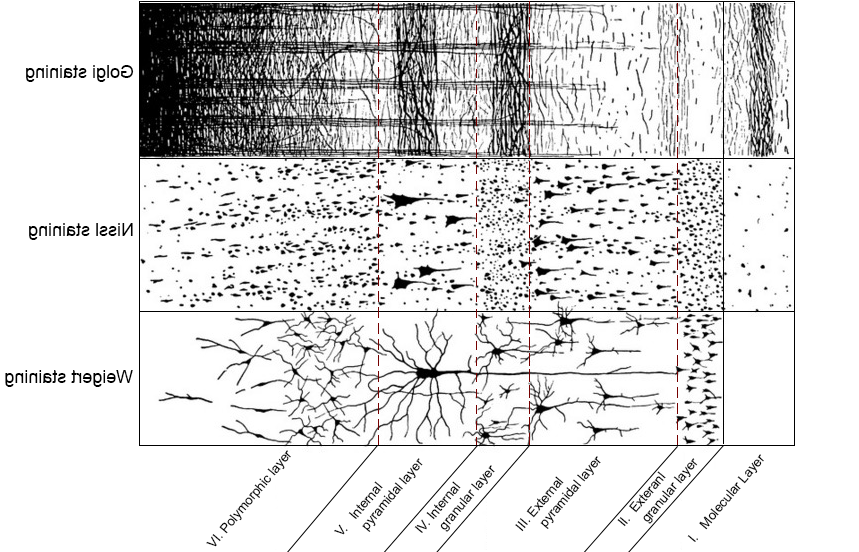
\includegraphics[width=0.8\textwidth, clip=true]{./Chapters/01_Introduction/Images/Layers}
	\caption{\cite{Brodman1909} }
	\label{fig:layers}
\end{figure}

For a small set of experiments, it is relatively straightforward to say if they are feed forward or feedback, but now think of more complicated processes: what would constitute as feed forward in language processing, decision making or memory? This is largely unknown and that is why it is of great interest to learn more about the laminar processing. It could shed light on a multitude of cognitive processes and open doors to a whole new type of information and new research in the brain \cite{Lawrence2017}. However, the greatest barrier is that is neuronal communication is not easily measured. With fMRI, only a derivative of neuronal firing can be measured as changes in oxygen consumption. We will therefore first need to get a better understanding of what type of information it is that fMRI can yield.

\section{Contrast Mechanisms}
Neurons clearly have layer specific functions, but measuring them is not easy, especially not in living humans. We cannot put electrodes in their heads, but what we can do is put them in an MRI scanner. An MRI scanner, however, cannot measure direct neuronal firing. Instead, it is susceptible to all kinds of magnetic properties of which three dimensional images can be made. Most notably, the magnetic susceptibility of red blood cells changes when they are oxygen rich or oxygen poor \cite{Ogawa1990}, which we call the Blood Oxygenation Level Dependant Signal, the BOLD signal. However, while there is little doubt that activation in a cortical region elicits a BOLD response, large parts of the biological mechanism behind it are still disputed. Most importantly, the extent to which the BOLD response reflects laminar specific activation is largely unknown. 

It was noted that maybe more so than just activity (MUA, multi unit acitvity), the amount of synaptic input (measured by the local field potential, LFP) migth be crucial for the strength of the BOLD response \cite{Goense2008}.

\begin{figure}[!ht]
	\centering
	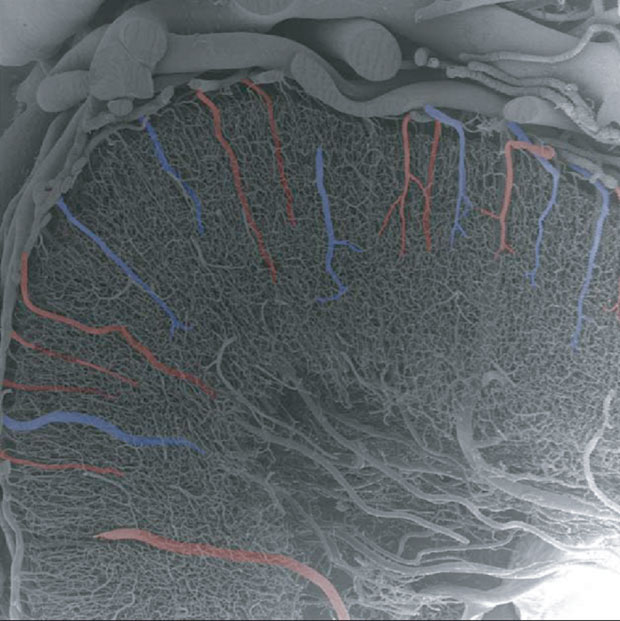
\includegraphics[width=0.9\textwidth, clip=true]{./Chapters/01_Introduction/Images/Microvasculature}
	\caption{The microvasculature of the visual cortex of a macaque \cite{Weber2008}. }
	\label{fig:microvasulature}
\end{figure}
Figure~\ref{fig:microvasulature} shows the microvasculature of a small piece of visual cortex in a macaque. In red, the arterioles, small blood vessels that dive from the top of the cortex (the pial surface) downward to supply the whole grey matter from blood. The smallest vessels, the capillaries, relay the oxygen to the neurons in all cortical layers, such that deoxygenated hemoglobin is drained away by the veins (blue). The veins on top of the cortex can be an order of magnitude larger than the cortical veins, and conduct off the deoxygenated blood. This might make one appreciate the difficulty of extracting laminar specific signals with large signals of non-interest in the direct neighbourhood. 

But the level of blood oxygenation is not the only quantity that fluctuates as a result of cortical activation. More blood starts flowing (higher cerebral blood flow, CBF), vessels start dilating (more cerebral blood volume, CBV) and the consumption of oxygen increases (higher cerebral metabolic rate of oxygen, CMR$_{O2}$). These quantitative measures can be related to one another by the Davis model, save some free parameters that need to be empirically determined \cite{Davis1997}. However, the proposed equations hold for the cortical column in its entirety, but does not take into account potential layer specific differences. 

So while we cannot measure neuronal activation with MRI, the closest we can get is the traces in the magnetic properties in the vasculature through BOLD, CBV, CBF, and CMRO$_{2}$. The extent to which these quantities vary as spatially specific as the level of the cortical layers is an outstanding question, however, and needs to empiraclly tested. Indeed, there are techniques to measure them, $T_2^*$-weighted imaging \cite{Norris2006} for BOLD, VASO for CBV \cite{Huber2018}, arterial spin labelling \cite{Grade2015} for CBV, and calibrated BOLD \cite{Blockley2013}) for CMRO$_{2}$. All vary in terms of sensitivity, specificity, and attainable resolution (spatial as well as temporal). The spatial resolution in combination with the type of experiment that is required for CBF and CMRO$_2$ measurements makes them poor candidates for human in vivo fMRI. It is mainly BOLD and CBV that have shown promising layer specific differences in animal experiments \cite{Lu2004,Zhao2006,Jin2008,Goense2012}. The main benefits of VASO compared to BOLD are its quantifiability \cite{Lu2003} and local specificity \cite{Jin2006}, whereas BOLD has higher sensitivity and speed \cite{Huber2018}.

Our main goal was to investigate the possibilities of laminar analysis in standard experiments on humans, and hence chose to use the BOLD signal as our signal of interest. Fundamentally, the BOLD signal arises as a consequence of magnetic field perturbations arising from desoxyhemoglobin molecules \cite{Norris2006}. These changes extend beyond the blood vessel and drop off as a function of field strength, the orientation of the vessel, and the vessel diameter. 
From the time that the molecules are excited until the time of the echo, molecules move around through the vessel. If the trajectory of a molecule in this time is small compared to the vessel size (and hence compared to the drop-off), there is little change in its surrounding magnetic field and the effect is reversible, a static effect. If on the other hand the molecule's trajectory is large, its surrounding magnetic field changes more drastically and unpredictably, such that the effect is irreversible and dynamic.
These two contrast mechanisms are the static and dynamic extravascular effect
The magnetic field perturbations scale linearly with field strength, so the trajectory of a molecule relative to the perturbations is much greater at 7 Tesla than at 1.5 Tesla. Thus, the dynamic extravascular effect increase with field strength. 
The remaining static effect at 7 Tesla is thus very specific, but detecting it requires high sensitivity \cite{Panchuelo2014}. 
An additional source of BOLD contrast is the intravascular effect. The magnetic field inside the vessel is slightly different from the surrounding tissue because of the amount of desoxyhemoglobin. As a result, the signal will start to dephase with respect to the extravascular signal. This is can be reversed because it is constant over time and is called the static intravascular effect. The exact origin of the last contrast mechanism is unclear. This is irreversible (dynamic) intravascular dephasing and has to do with the random movement of water molecules within red blood cells. It is either due to these water molecules interacting with the deoxyhemoglobin, or with the diffusion in and out of the cells, but no experiment to date has been able to tease the two mechanisms apart.
Four different contrast mechanisms can be distinguished.

Even given these four contrast mechanisms, it is still an outstanding question in what proportions they proliferate in measurements. This may even vary at the laminar level, as the deoxyhemoglobin from deeper layers flows upward to the top layers. The strengths of these effects have been modelled \cite{Markuerkiaga2016,Uludag2017} for both spin echo and gradient echo and suggest that most of the signal produced in a layer is also visible in that layer. For spin echo this is almost fully the case, while gradient echo has a tail that extents to more superficial layers, but at a gain of sensitivity. A range of laminar profiles has been found using spin echo (e.g. \cite{Zhao2004,Harel2006,Goense2006}), gradient echo (e.g. \cite{Polimeni2010,DeMartino2013,Chen2013}) or a combination of both, GRadient A Spin Echo (GRASE) \cite{Olman2012,DeMartino2013}.

Choosing a sequence requires carefully balancing the advantages and disadvantages against each other. We here chose to use gradient echo to investigate the laminar BOLD signal for its higher sensitivity at a field strength of 7 Tesla for high specificity. The potential downside of this is the susceptibility to the larger veins on top of the cortex that might obscure smaller effects \cite{Barth2007}. While the exact origins of the BOLD signal are unknown, there is strong evidence that the BOLD signal has a laminar footprint \cite{Logothetis2001}. Although some results from animal studies suggest that the effects may be visible at a higher temporal resolution than human in vivo MRI can achieve \cite{Yu2014,OHerron2016}. With the many uncertainties and the small size of the potential effect, it is soon clear that any potential effect can only be picked up with powerful methods that address as many sources of noise as possible. 

\subsection{Methods}
After covering the fundamentals of measurement techniques, it is clear what types of information may be expected to be present in the data. Getting out the relevant information, however, is at least as complicated. The brain is a highly convoluted structure that we are trying to describe and visualise by means of cubic voxel rasters. The first problem we encounter is a geometrical one: how do we attach a brain location to voxels in space? This can be done by making a \emph{cortical reconstruction} on a high resolution brain scan \cite{Dale1999,Bazin2012} with a very clear contrast between the white matter and grey matter as seen in Figure~\ref{fig:mybrain}. The distinction between white and grey matter is clear enough to draw a three dimensional boundary on both side of the grey matter: on the white matter boundary and one on the pial surface, the separation between the grey matter and the cerebrospinal fluid (CSF).
\begin{figure}[!ht]
	\centering
	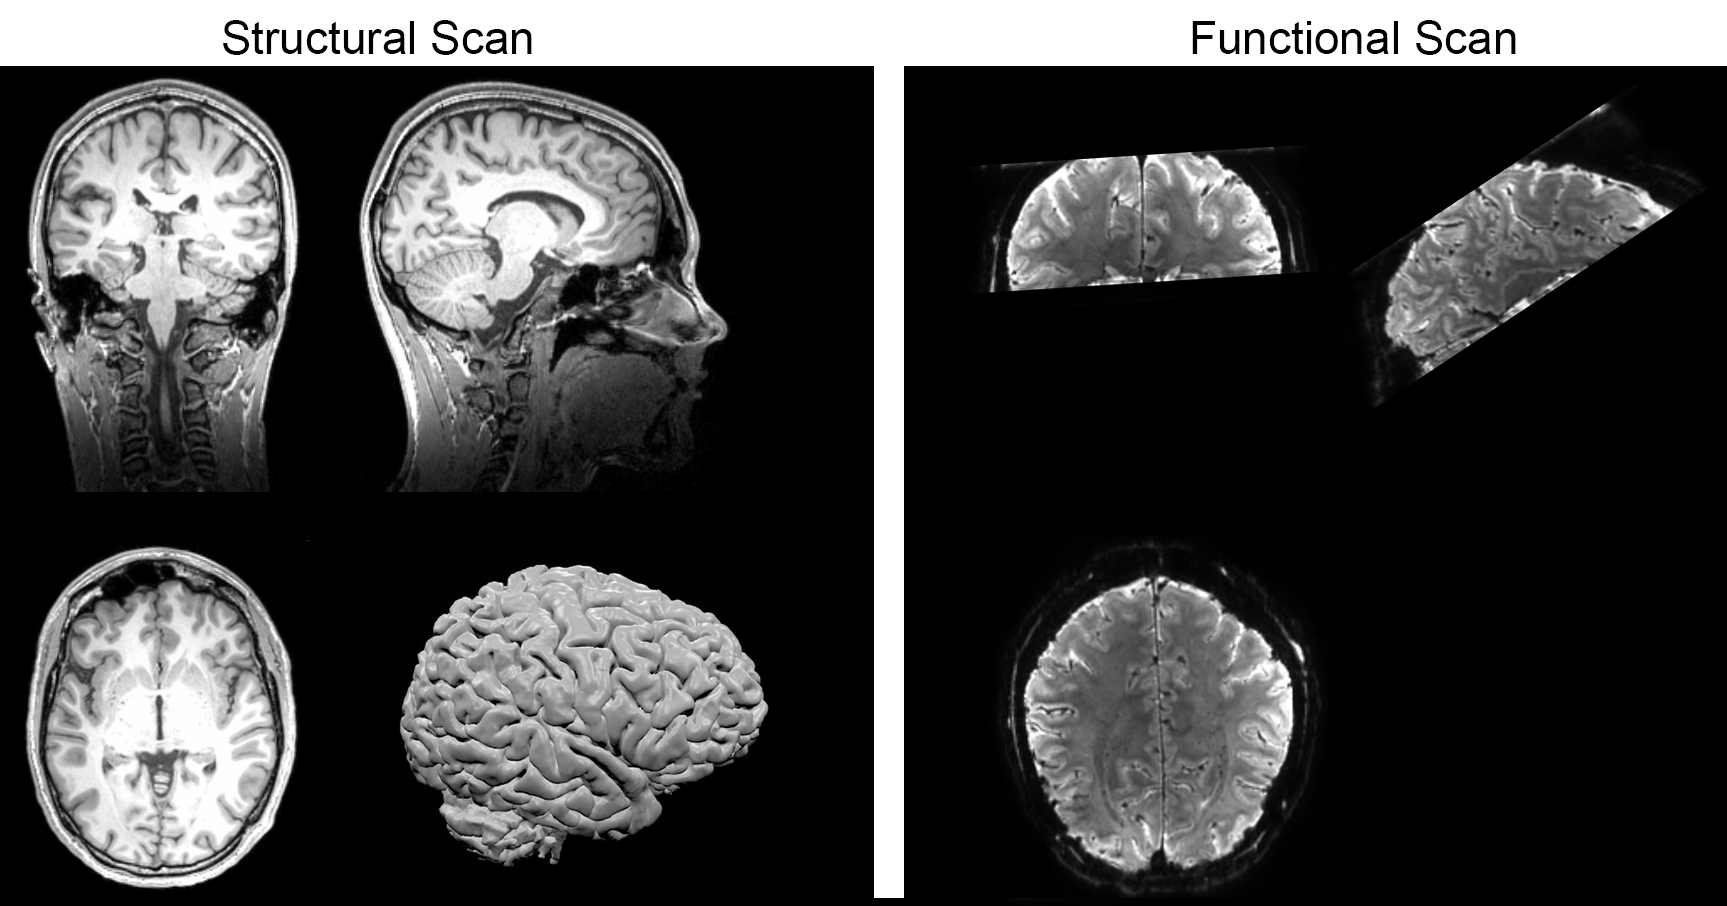
\includegraphics[width=0.99\textwidth, clip=true]{./Chapters/01_Introduction/Images/MyBrain}
	\caption{An example of a structural and functional brain scan. On the left, the structural scan has high anatomical contrast and sharp differences between the white matter and grey matter. The contrast is sharp enough to make a three dimensional reconstruction of the brain (lower right corner). On the right, a functional image is shown. The anatomical contrast is much weaker, but it can be acquired quickly and the contrast is susceptible to slight changes in blood deoxyhemoglobin, related to oxygen consumption on neuronal activation.}
	\label{fig:mybrain}
\end{figure}

The cortical reconstruction is very informative about the shape of the brain and potentially also about the layers: One could imagine different layers to be described as intermediate surfaces between both outer boundaries of which the locations can be used to then sample the cortical layers \cite{Koopmans2011,Polimeni2010,DeMartino2013}.
This descriptions allows for all sorts of surface base calculations \cite{Fischl2000,Bazin2012} and for example allows us to take into account a more naturalistic flow of the cortical layers \cite{Bok1929,Waehnertr2014}. Here it is described 



The people that we scan will move, breathe, fall asleep, ca
The scanner 


When we talk about a scanner with a field strength of 7 Tesla, it means there should be a homogeneous static magnetic field of that strength in the centre of the scanner. However, because the presence of a human body perturbs the field, it is not as homogeneous as one might want. Small perturbations can be corrected by \emph{shimming}, applying an additional magnetic field to compensate for the inhomogeneities. However, this is not accurate enough to correct all deviations and the inhomogeneities need not be constant over time. 


Distortion. The magnetic field is not always homogeneous



Multiple types 


It is possible geometrical properties 


%%
Balloon model \cite{Buxton1998}
something with a dynamic model of the hemodynamic signal \cite{Friston2000}.
















\section*{Thesis outline}
This thesis covers two major problems in laminar fMRI that needed to be solved before an experimental study could be conducted, and will reflect on building an fMRI pipeline, laminar or otherwise. In Chapter~\ref{ch:registration}, we will discuss a new way of coregistering an anatomical scan with a functional scan, when the latter is non-linearly distorted. We explain the details of the distortion correction technique, show its performance, and freely provide the code and data online. Chapter~\ref{ch:glm} describes a novel way of extracting laminar signal from data. We show its performance on a multitude of data, from a simulated fMRI model to post mortem data, to in vivo data from a set of subjects. Having overcome several of the most challenging aspects of laminar analysis, we then proceed to a laminar experiment in Chapter~\ref{ch:attention}. In a visual attention experiment, we investigate the laminar response. We further developped a new tool to more easily build fMRI analysis pipeline, to more reprodicibly conduct science, and to easily share analysis pipelines with others in Chapter~\ref{ch:porcupine}. Finally, these results will be put in a broader perspective in the Discussion, Chapter~\ref{ch:discussion}.


\linespread{1.5}
\newpage

%\linenumbers

\chapter{Improved cortical boundary registration for locally distorted fMRI scans}
%\chaptermark{Recursive Boundary Registration}
\label{ch:registration}

\textcolor{gray}{{Tim van Mourik$^{1}$}, Peter J Koopmans$^{2}$, David G Norris$^{1,2}$\\
$^{1}$Radboud University Nijmegen, Donders Institute for Brain, Cognition and Behaviour, Nijmegen, The Netherlands \\
$^{2}$Erwin L. Hahn Institute for Magnetic Resonance Imaging, University Duisburg-Essen, Essen, Germany}\\

%----------------------------------------------------------------------------------------
%	ABSTRACT
%----------------------------------------------------------------------------------------

\newpage
\section*{Abstract}
With continuing advances in MRI techniques and the emergence of higher static field strengths, submillimetre spatial resolution is now possible in human functional imaging experiments. This has opened up the way for more specific types of analysis, for example investigation of the cortical layers of the brain. With this increased specificity, it is important to correct for the geometrical distortions that are inherent to echo planar imaging (EPI). Inconveniently, higher field strength also increases these distortions. The resulting displacements can easily amount to several millimetres and as such pose a serious problem for laminar analysis.
We here present a method, Recursive Boundary Registration (RBR), that corrects distortions between an anatomical and an EPI volume. By recursively applying Boundary Based Registration (BBR) on progressively smaller subregions of the brain we generate an accurate whole-brain registration, based on the grey-white matter contrast. Explicit care is taken that the deformation does not break the topology of the cortical surface, which is an important requirement for several of the most common subsequent steps in laminar analysis. 
We show that RBR obtains submillimetre accuracy with respect to a manually distorted gold standard, and apply it to a set of human in vivo scans to show a clear increase in spacial specificity. 
RBR further automates the process of non-linear distortion correction. This is an important step towards routine human laminar fMRI. We  provide the code for the RBR algorithm, as well as a variety of functions to better investigate registration performance in a public GitHub repository, \url{https://github.com/TimVanMourik/OpenFmriAnalysis}, under the GPL 3.0 license.
\newpage
%----------------------------------------------------------------------------------------
\section{Introduction}
Investigation of the BOLD response with functional MRI at the level of the cortical layers has become increasingly popular over the the last decade \cite{Dumoulin2017,Trampel2017}. Activation levels differ at the laminar scale \cite{Koopmans2011} and they can vary depending on the performed task \cite{Muckli2015,Kok2016}. Laminar signals have the potential to reveal information about the underlying neuronal processes within a cortical region, as the signal from different layers may be associated with feed forward or feedback signals \cite{Felleman1991,Self2017}. However, layer specific analysis comes with great methodological challenges.

The thickness of the cerebral cortex varies between 1 and 4.5 millimetres \cite{Zilles1990,Fischl2000}. Identifying individual layers therefore ideally requires sub-millimetre resolution, at the cost of signal to noise ratio (SNR) per voxel. On top of this, a functional experiment ideally requires a Repetition Time (TR) on the order of several seconds. Layer specific investigations are hence best conducted at higher field ($\ge$7 Tesla) for improved SNR, but high field strength also have some disadvantages \cite{Poser2017}. The inhomogeneities of the static magnetic field $B_0$ can cause non-linear distortions when a fast acquisition scheme like Echo Planar Imaging (EPI) is used \cite{Mansfield1977}. Distortions primarily present themselves in the phase-encoding direction as a function of the bandwidth per pixel and static field strength \cite{Schmitt1998}. As layer specific analysis requires high spatial precision, non-linear distortions are particularly problematic. $T_2^*$-weighted images usually have insufficient contrast to segment the cortical grey matter, so instead one needs to identify the cortical boundaries from a different scan. This is typically a high-contrast $T_1$-weighted anatomical scan that can be segmented with tools such as FreeSurfer \cite{Dale1999}, CBS Tools \cite{Bazin2014}, or BrainVoyager \cite{Goebel2012}. However, as the anatomical scan is undistorted, it may not sufficiently overlap with the functional scan. 

Several potential solutions have been proposed for providing accurate alignment of functional images with an anatomical image. Early papers circumvent the problem by segmenting only a small piece of straight cortex \cite{Ress2007,Koopmans2010}. It is also possible to resort to different acquisition schemes like FLASH, which do not suffer significant distortions, but at a heavy cost in temporal resolution. Koopmans et al. combine this with a vertex based realignment procedure based on the Stripe of Gennari \cite{Koopmans2011}. This approach, however, is highly specific to parts of the primary visual cortex that show a myelinated band in the middle of the cortex (Stripe of Gennari), and does not generalise to the rest of the brain. Yet another alternative is to acquire an anatomical image with the same EPI readout and field of view as the functional image, such that the two volumes are similarly distorted \cite{Kashyap2017}. However, this (often unjustly) assumes that field inhomogeneities, and with it the distortions, do not change between acquisitions. Additionally, if the acquisition only covers a small part of the brain, cortical reconstruction algorithms may easily fail, as they are often based on whole-brain templates.

Ideally, there would be an accurate cross-contrast ($T_1$ to $T_2^*$) registration algorithm, but this is a notoriously hard problem. The combination of the warping of images and the unknown relation between contrasts creates a vast parameter space that is difficult to solve in a coregistration procedure. While algorithms like AFNI's \texttt{3dQWarp} \cite{Cox1996} technically support cross-modal cost functions, the documentation acknowledges that such usage is rather experimental and in our experience indeed does not reach submillimetre accuracy. In general, no algorithm currently exists that corrects non-linear distortions in high resolution low-contrast images up to the laminar specific level, and works either on partial or whole-brain images.

One way to search through relevant information in the image domain is to try and detect the grey-white matter boundary and match this between volumes. This is using \emph{geometric} information on top of \emph{volumetric} information and forms the basis of Boundary Based Registration (BBR) \cite{Greve2009}. A three-dimensional cortical reconstruction of the grey-white matter boundary is created on a high contrast anatomical image and serves as a basis for the coregistration. While a functional image is too low in contrast for generating a cortical reconstruction, it can be used in the registration procedure. The contrast is sufficient to optimise the average contrast across the boundary in order to achieve a better realignment. This was proposed for linear registrations and proven to be an exceedingly robust method. We here extend BBR to work recursively and effectively produce a cross-contrast non-linear registration. Our aim was to provide accurate submillimetre registration for whole-brain or partial brain images. The algorithms can be performed on the the functional data, without additional acquisition of additional scans, and without reinterpolation as a result of a non-linear warping. Importantly, the procedure produces a smooth deformation field that does not alter the topological properties of the mesh, such that the resulting surfaces can naturally be used in subsequent automatic layering and further layer specific analyes \cite{Waehnert2014,Leprince2015}.

\section*{Methods}
Boundary Based Registration (BBR) is based on a cortical construction of the boundary between the white matter and grey matter, and the grey matter and the CSF (pial surface) \citep{Greve2009}. This surface is generated on an anatomical scan, as the contrast of the functional scan may not be good enough for segmentation. In order to register the two volumes, the constructed surface is moved to the functional image. The average contrast across the grey-white matter boundary is computed and used as a cost function to optimise the transformation parameters of the registration. Versions of BBR are implemented in FreeSurfer (\texttt{bbregister}) \citep{Dale1999} and FSL (\texttt{flirt -cost bbr}) \citep{Jenkinson2001}. This method is powerful enough to be able to register the volumes, based on only a small part of the brain \citep{Greve2009}, suggesting that local application can also be successfully employed. Especially for high resolution (laminar) fMRI, the anatomical and functional volumes contain detailed information about the gyrification that can be used for registration. We hence propose to extend BBR with a hierarchical strategy \citep{Collins1995}. By recursively applying BBR at diminishing scales as a series of linear transformation, the volumes are effectively non-linearly registered.

The way in which the mesh is divided is based on a three-dimensional cuboid lattice consisting of the set of neigbourhoods $\mathcal{N}^{d}$ at various depths $d$, decreasing in size. At each depth, $\mathcal{N}^{d}$ is divided into eight equally sized cuboids (two in each dimension) $\mathcal{N}^{d + 1}$ until a user specified threshold size is reached. All vertices that make up the brain mesh are divided over the elements of $\mathcal{V}^{d}$, the set of vertices within $\mathcal{N}^{d}$. The number of vertices in each neighbourhood may well vary between regions.

Registration is performed iteratively, from the largest scale ($d=0$) to the smallest ($d=d_{max}$). For each element $\mathcal{N}_{i}^{d}$, a registration is computed by means of a boundary based registration algorithm \citep{Greve2009} applied to $\mathcal{V}_{i}^{d}$. In short, this is an edge detection algorithm that maximises the average contrast across the white matter surface. Contrast is defined as the (optionally weighted) gradient of samples on either side of vertices within the mesh. For the optimisation procedure we use MATLAB's gradient descent method \texttt{fminsearch} (default parameters) to optimise registration parameters as a function of contrast. The same sampling method and cost function were used as proposed by Greve \& Fischl \citep{Greve2009}.

Applying the computed transformations directly to $\mathcal{V}^{d}$ could easily `break the mesh' at the edges of neighbouring regions as their continuity is not guaranteed. This is a serious problem, as subsequent steps in laminar analysis (like the level set methods \citep{Sethian1999}) require the mesh to be a topological sphere: a non-intersection closed surface without holes. In order to ensure continuity we use a control point based strategy \citep{Collins1995}: let the edges and corners of $\mathcal{N}^{d}$ define a deformable lattice. For each computed transformation in $\mathcal{N}^{d}$, a resulting displacement vector is assigned to all of its corner points. After all transformations at a depth level are computed, the median is taken of all displacement vectors for each control point, thus representing a resultant vector based on adjacent neighbourhoods. In order to further increase robustness (but at the cost of specificity), the displacement vectors may subsequently be adjusted based on their direct neighbours:
\begin{equation}
\vec{d}=\alpha \vec{d} + \left(1-\alpha\right) \mathbf{M}(\vec{x}),
\label{eq:alphasmoothing}
\end{equation}
where $\mathbf{M}(\vec{x})$ denotes the mean displacement of the neighbourhood. Collins et al. \citep{Collins1995} experimentally found $\alpha=0.5$ yields an acceptable balance between local matching and global smoothness. We recommend higher values for $\alpha$, as our primary goal in laminar analysis is the local matching. We suggest additional ways of increasing robustness in the next section.

As all control points within $\mathcal{N}^{d}$ now have displacement vectors associated with them, $\mathcal{V}^{d}$ can be displaced proportionally to the distance to their closest control points. A way of describing this is by defining transformation matrix $\mathbf{T}$, such that it satisfies:
\begin{equation}
\mathbf{D}_{i}^{d}=\mathbf{T}\mathcal{V}_{i}^{d},
\label{eq:regression}
\end{equation}
where the set of displacement vectors is denoted by $\mathbf{D}^{d}$, for which each $i$'th element contains 8 vectors, one for each corner of the cube. This is a typical linear regression equation and could hence trivially be solved for $\mathbf{T}$. However, a least squares solution is required as the system is overdetermined with eight corner points and only a $[4 X 4]$ transformation matrix. This necessarily requires an approximation of the deformation vectors that may result in discontinuities with respect to adjacent neighbourhoods. A preferred method is to divide the cube into six tetrahedra by means of Delaunay triangulation \citep{Delaunay1934} and compute a separate matrix for each of them. For each tetrahedron, equation~\ref{eq:regression} represents a determined system, for which the solution for adjacent tetrahedra is guaranteed to be continuous. Effectively, this division increases the degrees of freedom of the deformation field to satisfy our requirement of continuity. Having found the transformations, they can readily be applied to adjust the position of $\mathcal{V}^{d}$.

This procedure is repeated for all depths levels $d$. Whenever the number of vertices in $\mathcal{N}^{d}$ is smaller than a user specified minimum, the transformation for that region is set to the identity matrix. 

\subsection*{Robustness}
\label{sec:robustness}
With the exponential increase in number of neighbourhoods as a function of depth level, the number of registrations easily reaches into the hundreds. The high number of Degrees of Freedom (DoF) of the algorithm therefore inescapably increases the probability of misregistrations. The algorithm ensures robustness and continuity in several ways, by computing displacement vectors as a weighted average of all surrounding neighbourhoods, and by an (optional) additional smoothing of displacement vectors based on adjacent control points, as mentioned above. Additionally, we compute a transformation within a neighbourhood not only for the entire neighbourhood, but also for six subregions. By splitting $\mathcal{V}^{d}$ separately into two in the $x$, $y$, and $z$ dimensions, six cuboids are created for which the registration is repeated. This procedure is  illustrated in Fig.~\ref{fig:cubedivision}. The resulting displacement vectors are added to the respective list for each control point. 
\begin{figure}[!ht]
\centering
\includegraphics[width=0.95\textwidth, clip=true]{./Chapters/02_Registration/Images/./WorkflowSchematic}
%\includegraphics[width=0.95\textwidth, clip=true]{./Chapters/02_Registration/Images/./Images/WorkflowSchematic.png}
\caption{
	A schematic of the workflow. First, the volume is recursively broken up into parts, for which registrations are computed by means of the edge detecting boundary based registration method. Based on the transformations found in this step, the second step is the updating of a cuboid lattice. The control points within the lattice are updated and applied to the boundaries. Specifically, this was performed based on a tetrahedral division of the cube. For each tetrahedron, a displacement field was computed and applied to the vertices within the tetrahedron.
}
\label{fig:cubedivision}
\end{figure}

\subsection*{Parameters}
The algorithm can look for any combination of translation, rotation and scaling in the $x$, $y$, and $z$ dimensions. It will divide the volume until it reaches a user defined minimum size or number of vertices, and a transformation will be computed. We here focus on registration in the phase enconding direction only, i.e. translation and scaling in the $y$-direction, as this is the most common type of distortion when an Echo Planar Imaging sequence is used \citep{Mansfield1977}. We set the minimum size of a neighbourhood to 4 voxels and the minimum number of vertices to 100. The smoothing factor with respect to adjacent vertices in the lattice from Eq.\ref{eq:alphasmoothing} was set to $\alpha=0.9$. Experimentally, we have found that this still yields robust results while still being highly weighted towards specificity. In contrast, Collins et al. \citep{Collins1995} describe an $\alpha$-level of $\alpha=0.5$, which is likely to do with the fact that their purpose of template matching and segmentation prioritises robustness over specificity. While the original implementation of BBR recommends using subsets of vertices for parts of the algorithm \citep{Greve2009}, we here use all vertices at all stages. This may be redundant for registrations at the large scale, but as it is a small addition in computation time, and because errors in early iterations may propagate further downwards, we chose to incorporate all vertices. Finding the best selection of parameters may still require some iterations for a given data set. It is, however, a substantial improvement with respect to the arduous job of manually matching small patches of cortex within a very limited field of view. 

\subsection*{Validation}
Assessing the quality of the registration performance proved challenging. While there is a clear theoretical relationship between the distortion size and the parameters of the acquisition \citep{Jezzard1995}, in practice it is difficult to find a gold standard for the submillimetre accuracy that we are aspiring to. Tools to convert a field maps to estimates of voxel displacement are usually heavily smoothed and cannot account for subject movement in the scanner or field changes between acquisitions. We hence created our own gold standard by acquiring an undistorted FLASH image and manually distorting it based on a field map. This way, the exact distortions were known in order to test if we could find them back with RBR. 

% % FLASH fieldmap
A high resolution whole brain multi-echo FLASH image \citep{Haase1986} was acquired at a 3T Siemens Scanner, TR=95 ms, $\alpha$=20\textdegree, bandwidth=170 Hz/px, [0.75 mm]$^3$. GRAPPA was used for three-fold in-plane acceleration. The echo times ranged from 5.88 ms to 78.96 ms with an echo spacing of 8.12 ms. The average of the last seven echoes was used, as the first three contained little contrast. This was accompanied by a whole brain MPRAGE acquisition that was used for the FreeSurfer cortical reconstruction, TR/TE/TI/$\alpha$ = 2300 ms/3.15 ms/1100 ms/8\textdegree, [0.8 mm]$^3$. A field map was acquired to realistically distort the FLASH image. The resolution was [3.5 mm X 3.5 mm X 2.0 mm], TR/TE1/TE2/$\alpha$ = 1020 ms/10 ms/12.46 ms/90\textdegree, bandwidth=260 Hz/Px.

The cortical reconstruction from FreeSurfer's \texttt{recon-all} \citep{Dale1999} was coregistered to the FLASH image using a 6 DoF linear registration with a custom MATLAB implementation of BBR. In order to distort the cortical surface, a voxel displacement map (VDM) was computed using SPM field map tools \citep{Andersson2001}. 
In order to taper unrealistically large displacements, and to move non-displaced vertices away from zero, the VDM was first transformed by a cubic root, after which it was applied in the anterior-posterior direction to the boundaries. Vertices were on average displaced by 2.56 mm (3.4 voxels), which is considerably more than could be tolerated for a laminar specific experiment. The distribution of displacement values was bimodally distributed away from zero with the specific goal to let RBR find the displacement and yield a sharp unimodal distribution around zero, as close to a delta distribution as possible.

% % EPI real
Additionally, RBR was tested on 12 brain scans obtained from a 7T scanner. We used 3D EPI \citep{Poser2010}, [0.93 mm]$^3$, TR/TE/$\alpha$ = 2768 ms/20 ms/14\textdegree, bandwidth=1167 Hz/pixel, phase encoding direction: A -> P, matrix size = 204$^2$, effective echo spacing = 0.25 ms. The boundaries were created by FreeSurfer on a whole-brain MP2RAGE (1.03 mm$^3$, TR/TE/TI1/TI2 = 5000 ms/1.89 ms/900 ms/3200 ms) \citep{Marques2010}. BBR was performed by \texttt{bbregister} with a full affine transformation (12 DoFs) on the mean of the functional images and subsequently, the boundaries were imported to MATLAB. Overlaying the registered boundaries on top of the EPI image showed clear local geometrical distortions in the phase encoding direction, related to field inhomogeneity \citep{Jezzard1995}. These distortions were of the order of several millimeters within a single volume. We corrected this with RBR and investigated its performance.

It must be noted that it is challenging to find an objective metric by which the quality of the registration could be quantified. The true distorted position is unknown and methods to approximate do not have the desired submillimetre specificity that is required. Moreover, if such metric existed, it could itself be used in the optimisation procedure. An alternative, however, is an investigation of RBR's performance on the true volume compared to the performance on the volume with different levels of added noise. Assuming that the algorithm has the best performance on the original data, the displacement with respect to the no-noise condition is expected to increase when more noise is added. Note that this does not make a statement about the correctness of the result. To investigate the RBR's performance in the presence of noise, we added twelve different levels of white noise to the data, applied RBR and compared the displacement to the unsalted version. For this, we used the Average Absolute Distance (AAD) \citep{Greve2009}, defined to be the average distance that the cortical surface moves between the two sets of registrations.

\section{Results}
We employed RBR on a constructed gold standard where the exact displacement was known. By taking an undistorted FLASH image and realistically distorting the cortical surface by means of a field map, we could test if we could retrieve the initial position of the boundaries. In Fig~\ref{fig:registrationhistogram}, we present a histogram of the displaced boundaries and the registered boundaries, both with respect to the true position. The registered boundaries clearly show a sharp distribution centred around the origin ($\mu=0.027$ mm). The FWHM of the distribution is $0.49$ mm, showing that RBR provides accurate submillimetre registration. Additionally, Fig.~\ref{fig:flashregistration} shows a cross section (middle slice of the volume) of the registration.
\begin{figure}[!ht]
\centering
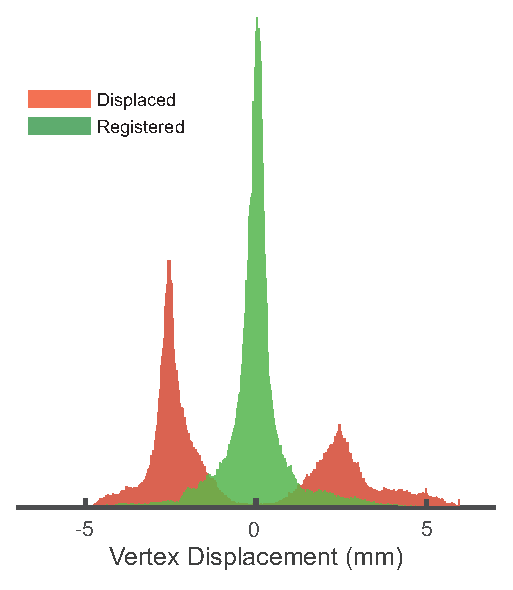
\includegraphics[width=0.4\textwidth, clip=true]{./Chapters/02_Registration/Images/./Histograms}
%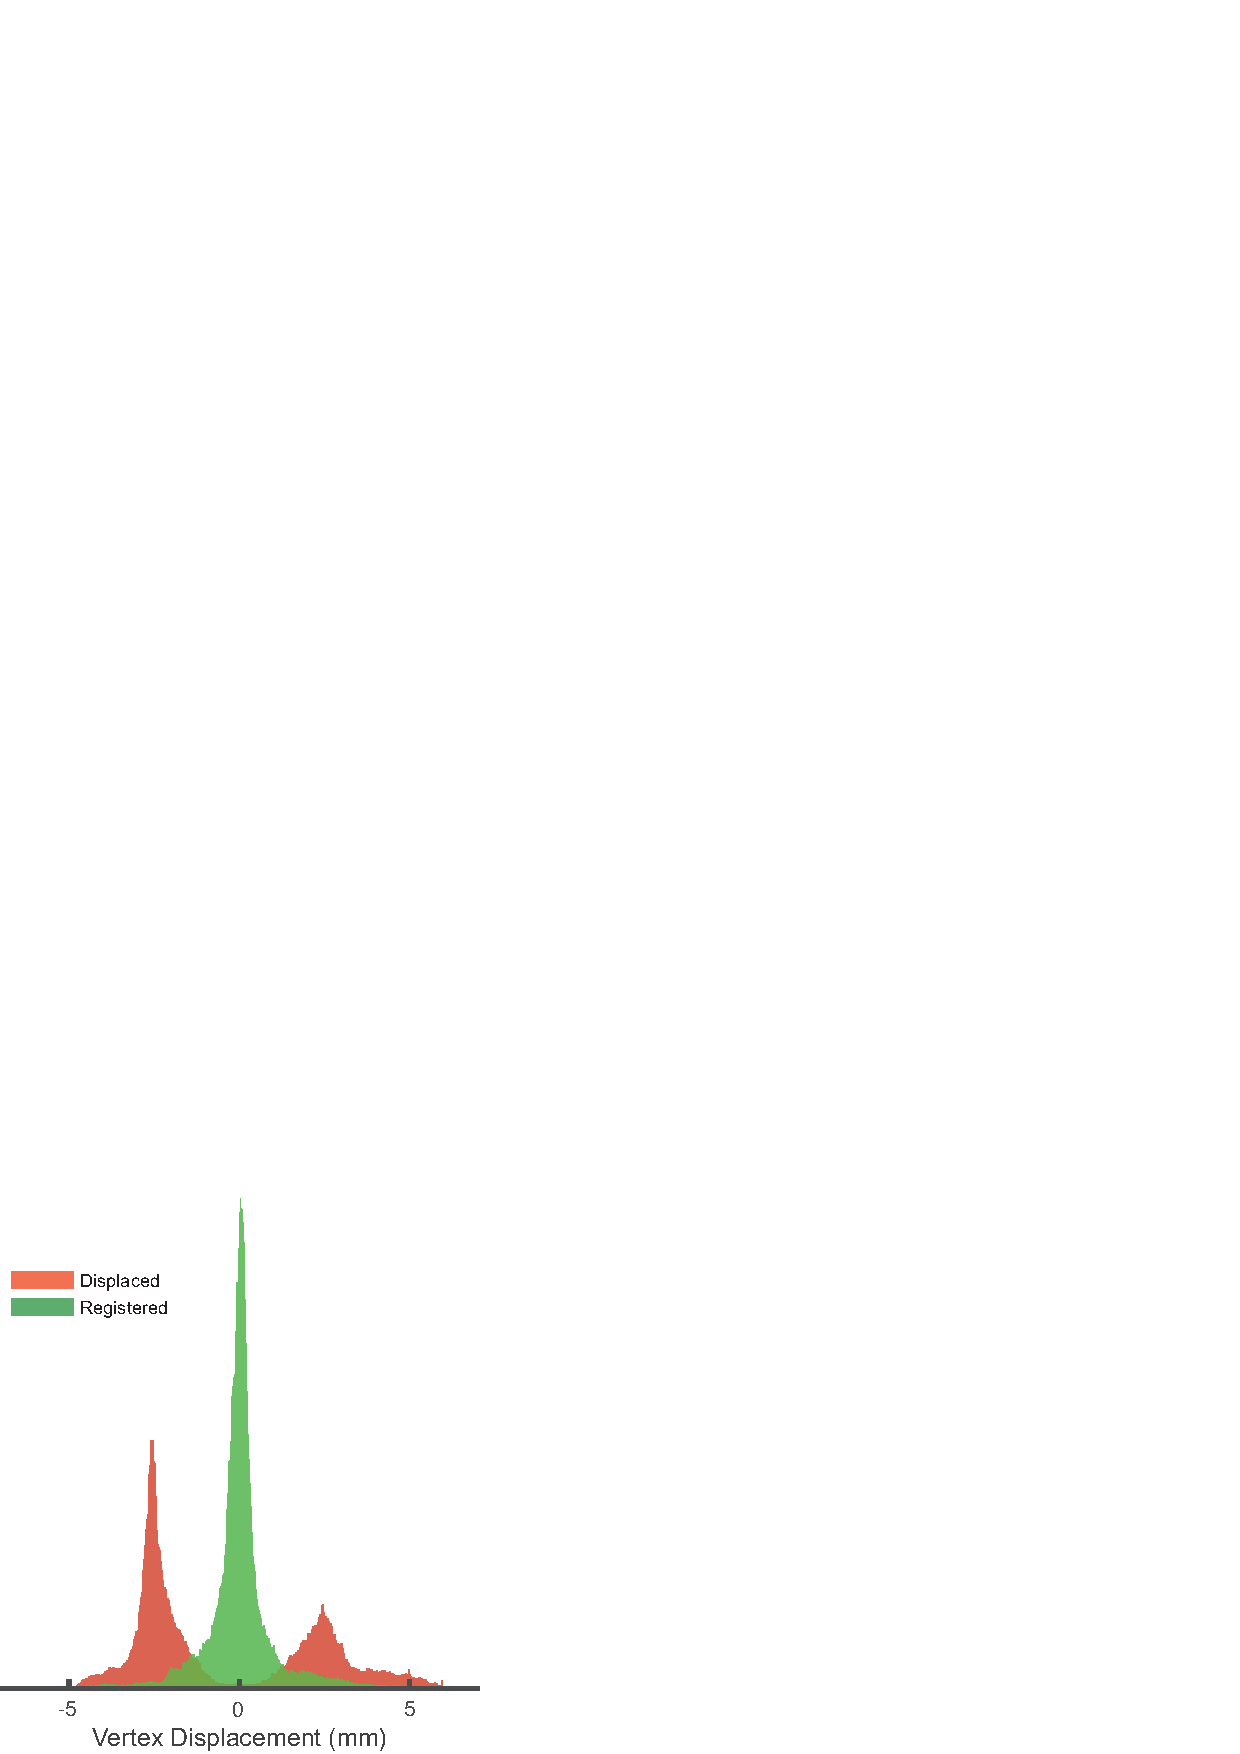
\includegraphics[width=0.4\textwidth, clip=true]{./Chapters/02_Registration/Images/./Images/Histograms.png}
\caption{Histogram of the displacement of all 228,208 vertices within a single brain mesh. The {\color{red}red} histogram shows the displacement after fieldmap based distortion with respect to a gold standard. The {\color{green}green} shows the displacement after applying RBR with respect to the same standard. After registration, the histogram clearly shows a sharp zero-centered (no bias) distribution.}
\label{fig:registrationhistogram}
\end{figure}
\begin{figure}[!ht]
\centering
\includegraphics[width=0.9\textwidth, clip=true]{./Chapters/02_Registration/Images/./FLASH_registration}
%\includegraphics[width=0.9\textwidth, clip=true]{./Chapters/02_Registration/Images/./Images/FLASH_registration.png}
\caption{The mid slice of the registration performed on a manually distorted FLASH image (red boundaries). The registered surface (yellow) overlaps for the larger part of the brain almost perfectly with the gold standard (green). If the specificity is set to high values, there is a risk that errors start to appear in some low contrast regions. This largely depends on the balance between false positives and false negatives in terms of corrected regions.}
\label{fig:flashregistration}
\end{figure}

In most of the slice (and the volume), the registration accuracy is well within the submillimetre regime. However, especially in low contrast areas the algorithm may show some small inaccuracies. This mainly proliferates when there is also another gradient in the image (e.g. the pial surface) on which the algorithm starts to fix the boundaries. This is largely related to the fine line between obtaining sufficient specificity and overfitting the data.

% % EPI
We performed RBR on a (resting state) dataset intended for laminar analysis consisting of 11 subjects. The boundaries after a 12 DoF \texttt{bbregister} were recursively registered to the mean EPI images (0.93 mm isotropic resolution) and this yielded an updated cortical surface. The new surface followed the grey matter boundary in the volume visibly better than the unregistered one. In Fig.~\ref{fig:epiregistration} we present a single slice with both sets of boundaries overlaid on top of them, illustrating the improvement. We here present the data for a representative subject, and identical images for all other subjects are presented in the Supplemental Materials.
\begin{figure}[!t]
\centering
\includegraphics[width=0.7\textwidth, clip=true]{./Chapters/02_Registration/Images/./EpiRegistration}
%\includegraphics[width=0.8\textwidth, clip=true]{./Chapters/02_Registration/Images/./Images/EpiRegistration.png}
\caption{
	Distortion correction of 7T 3D EPI data, obtained with 0.93 mm isotropic resolution. In {\color{red}red}, the original brain surfaces are shown after a 12 DoF registration performed by \texttt{bbregister}. The mesh in {\color{green}green} is the updated mesh by means of the first stage RBR, 2 DoF (scale and translation in the PE direction). The green boundaries follow the white matter boundary much better. The voxel displacement map (lower right) shows displacements on the order of several millimetres. The control point lattice that was used to displace the boundaries are overlaid onto the displacement map. Similar images for all subjects can be found in the supplementary materials. For even better inspection, movie files for all subjects are included in the online supplemental materials.} 
\label{fig:epiregistration}
\end{figure}

Additionally, Fig~\ref{fig:aad} shows the Absolute Average Displacement (AAD) of the registration on salted images with respect to the registration on the no-noise volume. Even for highly noisy images, the registration improves somewhat with respect to the undisplaced boundaries. In the absence of a gold standard model of the distortions, the monotonic decrease of the AAD indicates that RBR converges to an optimum as a function of data quality.
\begin{figure}[!ht]
\centering
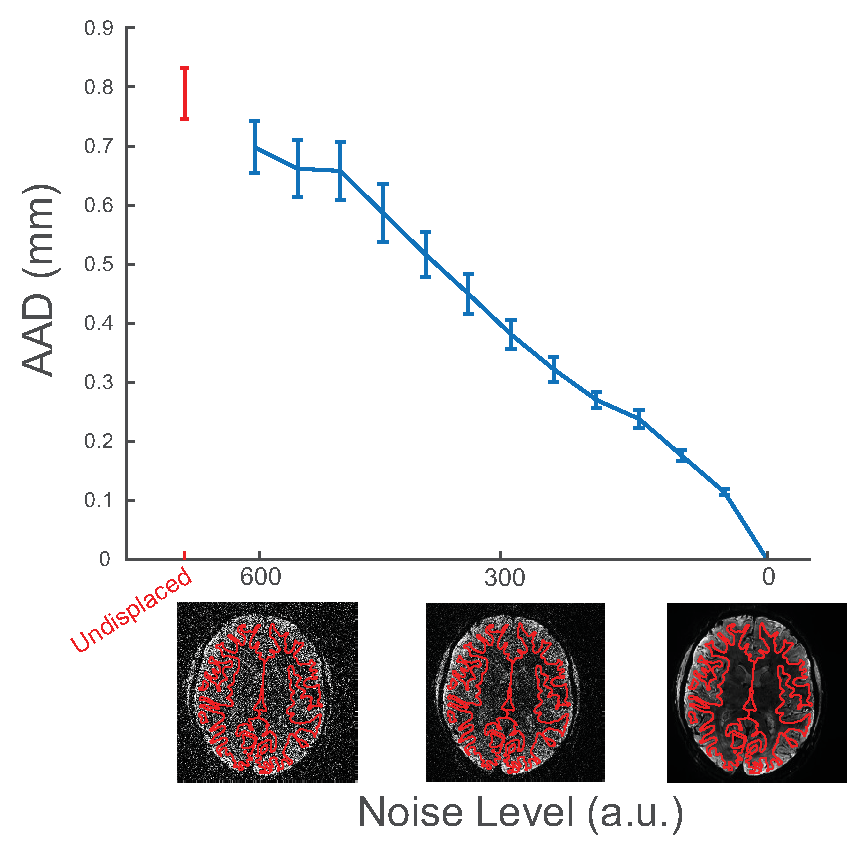
\includegraphics[width=0.7\textwidth, clip=true]{./Chapters/02_Registration/Images/./AAD}
%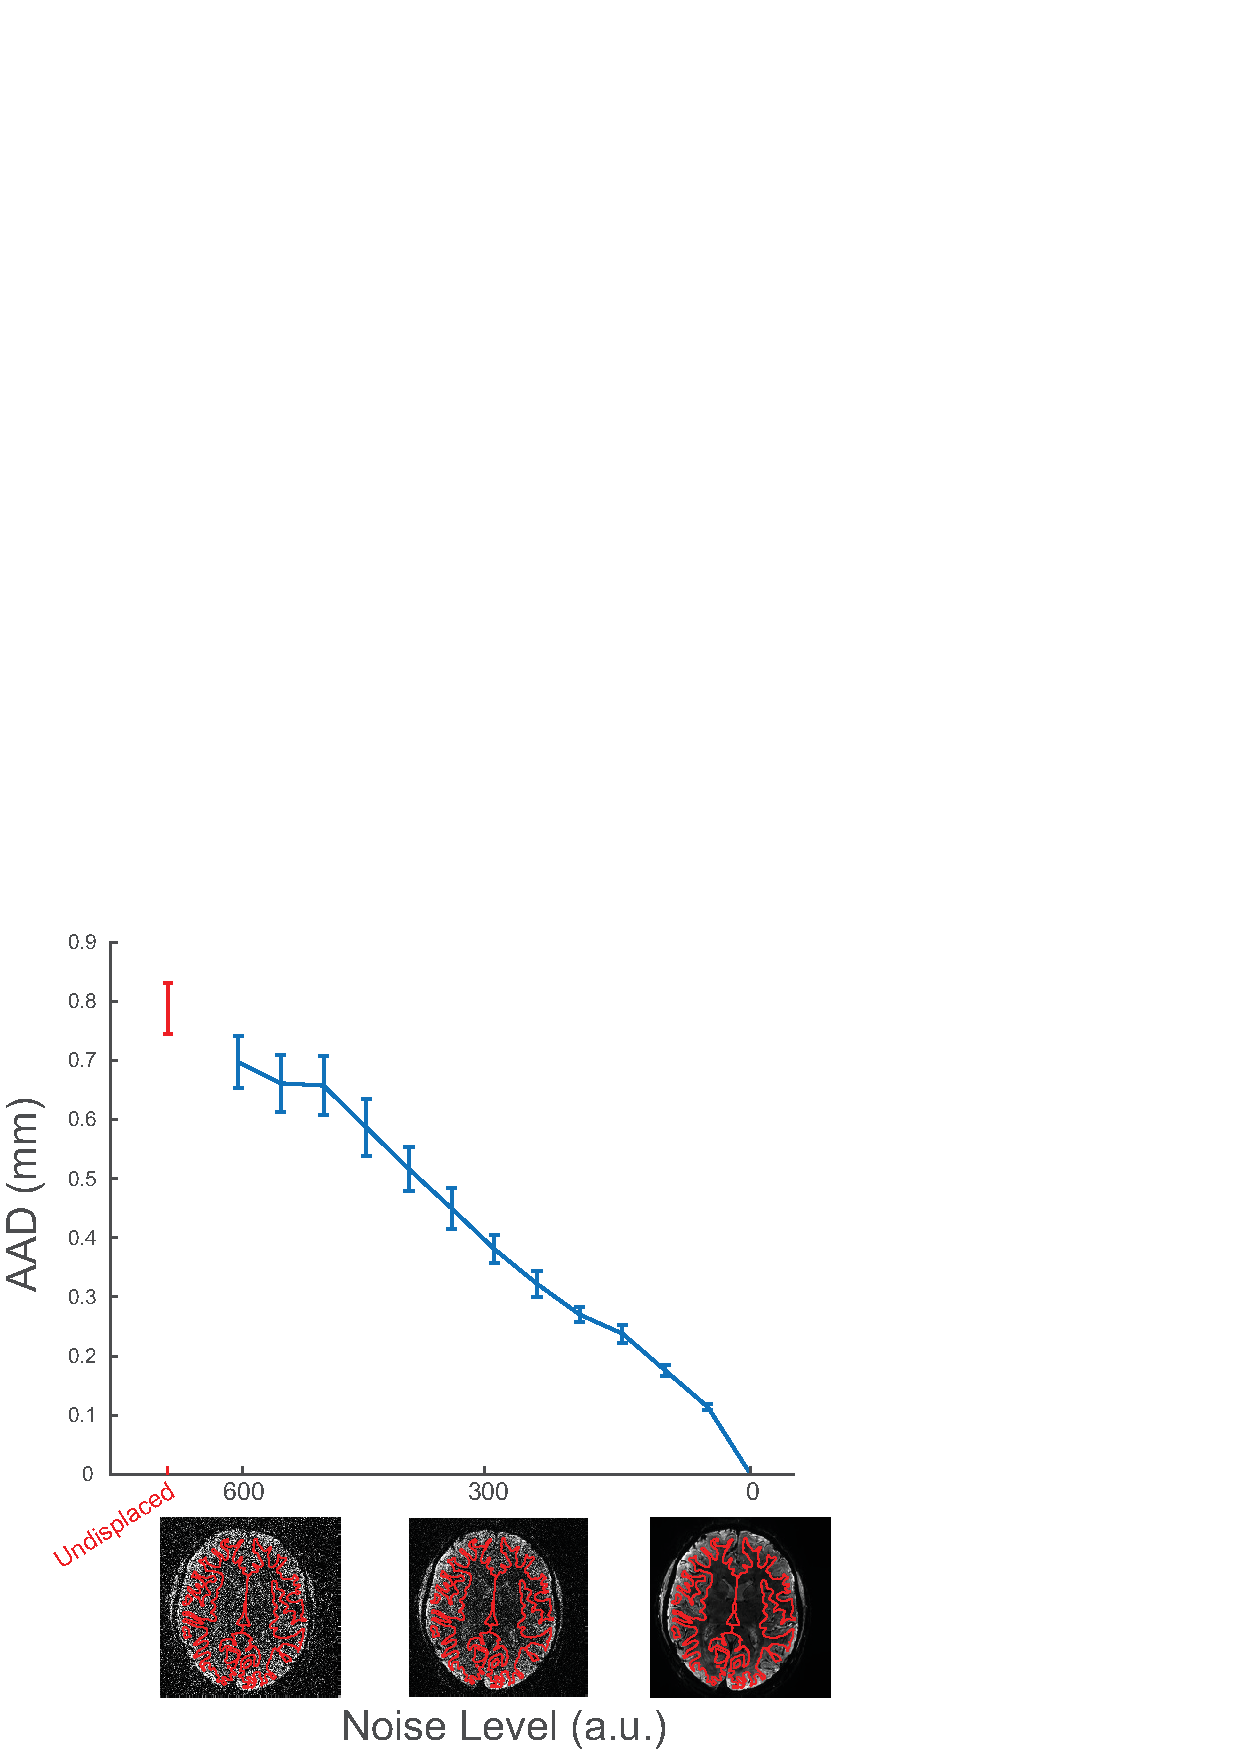
\includegraphics[width=0.7\textwidth, clip=true]{./Chapters/02_Registration/Images/./Images/AAD.png}
\caption{
	The effect of adding noise on the computed average absolute displacement with respect to a no-noise registration. In the absence of knowledge about the true distortions, the monotonic decrease of the AAD indicates that RBR converges to an optimum as a function of data quality.}
\label{fig:aad}
\end{figure}

\subsection{Data Availability}
All source code for the registration algorithm is freely available under the GPL 3.0 license at \url{https://github.com/TimVanMourik/OpenFmriAnalysis}. The respective modules are also available in Porcupine \url{https://timvanmourik.github.io/Porcupine}, a visual pipeline tool that automatically creates custom analysis scripts \cite{VanMourik2017}. All code to generate the images in this paper are available at the Donders Repository \url{https://data.donders.ru.nl/collections/shared/di.dccn.DSC_3015016.05_558/id/27015532}. This also includes additional movie files that scroll through the volumes, which is highly relevant to fully investigate whole brain registration performance. See Fig.~\ref{fig:si-qrcodes} for QR codes to the relevant links. 
\begin{figure}[!ht]
\centering
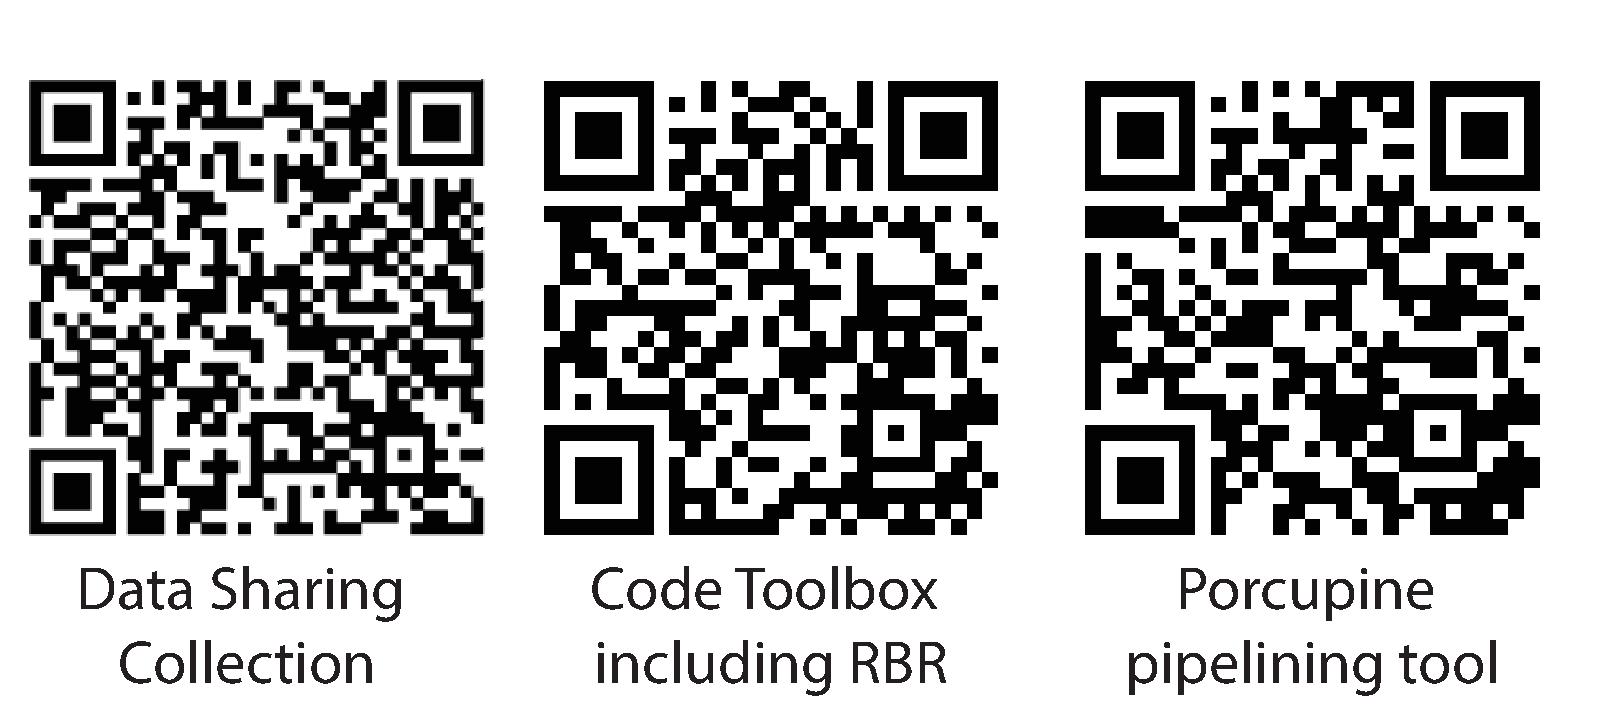
\includegraphics[width=0.3\textwidth, clip=true]{./Chapters/02_Registration/Images/./QRCodes}
%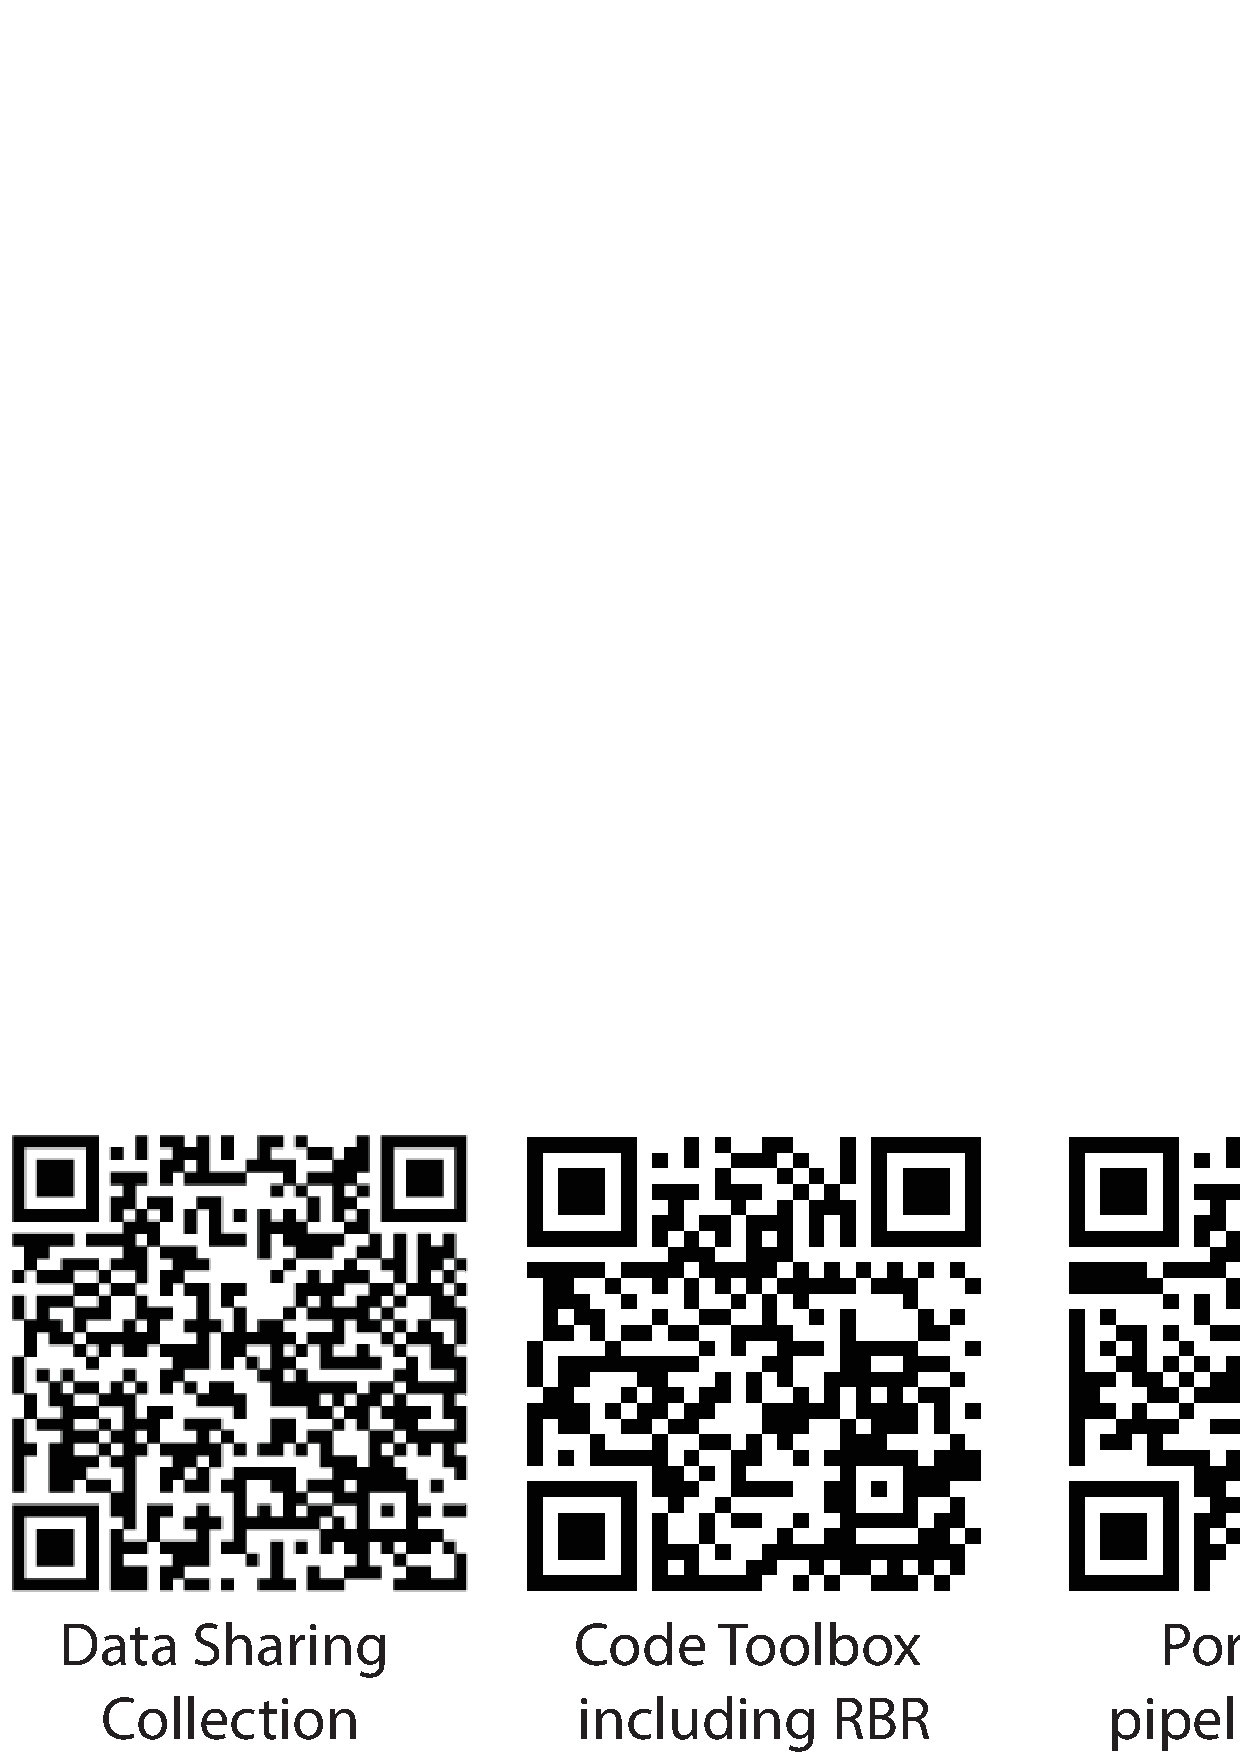
\includegraphics[width=0.5\textwidth, clip=true]{./Chapters/02_Registration/Images/./Images/QRCodes.png}
\caption{The links to, respectively, the source code of the algorithms, the analysis scripts for creating all figures in this paper, and the pipeline tool to easily incorporate it in one's custom analysis.}
\label{fig:si-qrcodes}
\end{figure}



\section*{Discussion and conclusions}
In recent years, laminar specific fMRI analysis has come in reach for human in vivo experiments. Where standard fMRI analyses are done on a routine basis, this is hardly the case for layer specific analysis, not least because OF the large amount of manual work that is involved. Aligning volumes to adjust for subject motion and non-linear distortion is one of the most challenging parts of the pipeline. With Recursive Boundary Registration (RBR) we here propose a solution to this problem by means of a recursive application of Boundary Based Registration. By using a control point lattice that forms the basis of deforming the mesh, the topology of the surface is preserved. This way, the mesh can easily be fed into next steps in making a cortical layering (Level Set Method) where it is an absolute necessity that the mesh is not broken as a result of the transformations. Due to the large number of degrees of freedom that is required to non-linearly deform a volume, we built in several methods to increase robustness. Nonetheless, as a mathematical certainty, increasing the sensitivity will increase the false positive rate, i.e. the risk of overfitting. It is up to the user to find the desired balance between them in the settings that we provide to control this balance. 

To ensure the functionality of this method, several conditions have to be met. A good reconstruction of the cortical surface is essential, as any inaccuracies will directly affect the contrast estimation and hence the registration optimisation. As the algorithm is based on edge detection, the volume to which it is registered needs to have sufficient contrast between white and grey matter. Furthermore, RBR is recommended to be initialised by a linear BBR registration. While RBR excels at subtle non-linear deformations, large displacement at any level may not be found in a rough multidimensional landscape through which the gradient descent method has to find it way to a minimum. In general, a gradient descent method may be difficult to monitor as it is susceptible to local minima trapping. A more robust algorithm may be a good improvement to RBR (e.g. using bounded gradient descents, or Monte Carlo sampling). Additional points of improvement could be the way in which the control point lattice is applied. While the subdivision into tetrahedra guarantees continuity across segments, it has a non-symmetrical orientation. The resulting displacement hence may show a residual bias as a result of the division. A smoother curve fitting technique to replace the current tetrehedral solution may be a valuable improvement, for example a diffeomorph version as implemented in ANTS \citep{Avants2011}. 

This algorithm in its current implementation focuses only on the \emph{gradient} around the gray and the white matter, without looking at the intensity value. One could imagine this to be problematic when the RBR is applied to a volume where a similar gradient of the same direction is present, for example the grey matter to CSF gradient. The algorithm may easily get `confused' about which boundary it needs to converge on. In $T_2^*$-weighted images in functional studies, this is not usually a problem as the grey matter has a higher intensity value than both CSF and white matter. However, in standard anatomical scans with $T_1$ contrast, this is not the case. As a result, RBR may fail due to the great similarity of contrast along both sides of the grey matter. An obvious extension for future use could be to use more prior knowledge about the intensity (as apposed to merely the gradient), in order to inform the algorithm which boundary it should use. With the open source and modular way the code is written, the cost function, optimisation algorithm or deformation algorithm could easily be replaced with improved versions, to accommodate ongoing development. 

A common use of non-linear registration is template matching, for example in an anatomical-to-MNI normalisation. RBR has little potential for this type of usage as it is based on finding fine within-subject similarities in a volume, rather than the coarser type of between-subject similarities. More probable potential use cases may be could in the matching of subcortical brain structures that are described with a three-dimensional mesh. Similarly, there is a wide range of more deformable parts of the body (e.g. liver, heart, stomach, etc.) that might benefit from solutions like RBR. 

We have shown that RBR automates the process of non-linear distortion correction in order to accommodate an extremely high specificity. This is a next step in automated processing of laminar analysis and more routine layer research. We have shown this yields submillimetre accuracy of registration. Finally, we concur with Saad \citep{Saad2009} and Greve \citep{Greve2009} in their conclusion to encourage visual inspection of the registration before reliance is placed on its accuracy.








\section{Supporting Information}
\label{SI}
These are single slice images of the registration performance for all other 10 subjects. More detailed information can be found in the online supplementary materials.
\begin{figure}[!ht]
\centering
\includegraphics[width=0.95\textwidth, clip=true]{./Chapters/02_Registration/Images/./SupplementRegistrations}
%\includegraphics[width=1.0\textwidth, clip=true]{./Chapters/02_Registration/Images/./Images/SupplementRegistrations.png}
\caption{
	Distortion correction of 7T 3D EPI data, obtained with 0.93 mm isotropic resolution. In {\color{red}red}, the original brain surfaces are shown after a 12 DoF registration performed by \texttt{bbregister}. The mesh in {\color{green}green} is the updated mesh by means of the first stage RBR, 2 DoF (scale and translation in the PE direction). The green boundaries follow the white matter boundary much better. For better inspection, the online supplemental materials include movie files that scroll through the volume. The voxel displacement map (lower right) shows displacements on the order of several millimetres. The control point lattice that was used to displace the boundaries are overlaid onto the displacement map.} 
\label{fig:si-registrations}
\end{figure}
\section*{Acknowledgements}
The authors would like to thank Irati Markuerkiaga for helping with collecting (and recollecting) the FLASH data set. Tim van Mourik acknowledges support by the Spinoza grant [SPI 40-118].

\chapter{Laminar signal extraction over extended cortical areas by means of a spatial GLM}
\chaptermark{Spatial GLM}
\label{ch:glm}

\textcolor{gray}{{Tim van Mourik$^{1}$}, Jan PJM van der Eerden$^{1}$, Pierre-Louis Bazin$^{2}$, David G Norris$^{1,3}$\\
$^{1}$Radboud University Nijmegen, Donders Institute for Brain, Cognition and Behaviour, Nijmegen, The Netherlands \\
$^{2}$Spinoza Centre for Neuroimaging, Amsterdam, the Netherlands \\
$^{3}$Netherlands Institute for Neuroscience, Amsterdam \\
$^{4}$Max Planck institute for Human Cognitive and Brain Sciences, Leipzig, Germany \\
$^{5}$Erwin L. Hahn Institute for Magnetic Resonance Imaging, University Duisburg-Essen, Essen, Germany}\\

%----------------------------------------------------------------------------------------
%	ABSTRACT
%----------------------------------------------------------------------------------------
\linespread{1.5}
\newpage
\section*{Abstract}
There is converging evidence that distinct neuronal processes leave distinguishable footprints in the laminar BOLD response. However, even though the achievable spatial resolution in functional MRI has much improved over the years, it is still challenging to separate signals arising from different cortical layers. In this work, we propose a new method to extract laminar signals.
We use a spatial General Linear Model in combination with the equivolume principle of cortical layers to unmix laminar signals instead of interpolating through and integrating over a cortical area: thus reducing partial volume effects. Not only do we provide a mathematical framework for extracting laminar signals with a spatial GLM, we also illustrate that the best case scenarios of existing methods can be seen as special cases within the same framework. 
By means of simulation, we show that this approach has a sharper point spread function, providing better signal localisation. 
We further assess the partial volume contamination in cortical profiles from high resolution human ex vivo and in vivo structural data, and provide a full account of the benefits and potential caveats. We eschew here any attempt to validate the spatial GLM on the basis of fMRI data as a generally accepted ground-truth pattern of laminar activation does not currently exist.
This approach is flexible in terms of the number of layers and their respective thickness, and naturally integrates spatial regularisation along the cortex, while preserving laminar specificity. Care must be taken, however, as this procedure of unmixing is more susceptible to sources of noise in the data or inaccuracies in the laminar segmentation.

\newpage
%----------------------------------------------------------------------------------------
\section{Introduction}
%The field
With functional Magnetic Resonance Imaging (fMRI) neuronal activity in the brain is measured indirectly via the Blood Oxygen Level Dependent (BOLD) response. With the emergence of higher static magnetic fields, more powerful acquisition sequences and better analysis tools, the location of the activation can be pinpointed  more  precisely. The attainable spatial resolution can be \add{so high that voxels are} smaller than the thickness of the cerebral cortex. These improvements have made it possible to investigate specific cortical layers with fMRI.
Typically the human cerebral cortex consists of six \change{histological}{cytoarchitectonic} layers \cite{Brodmann1909}. Layer IV is commonly associated with receiving feedforward input from Layer III from lower cortical areas or from the thalamus \cite{Jones1998}, while Layers II-III and VI are implicated in receiving downward information flow (feedback) \cite{Alitto2003}, which often originates from layer V. Layer I is thin and sparsely populated with neurons and will probably remain elusive to laminar fMRI. 

% Recent work
It is clear that there may be a lot of information about laminar processing in fMRI measures. The BOLD signal has convincingly been shown to have a laminar origins in the rat motor- and somatosensory cortices \cite{Yu2014}. Further tight spatial coupling has been demonstrated of blood flow and dilation of arterioles of layer II/III and orientation tuning in the cat visual cortex \cite{OHerron2016}. And in line with previous depth-dependent electrode recordings, the BOLD response that uniquely reflects trial by trial variance in the alpha and gamma bands was recently shown to be consistent with infra- and supra-granular origins of these oscillations \cite{Scheeringa2016}. While the details of the neurovascular coupling are still unknown \cite{Uludag2017}, \change{it has long been accepted that the BOLD response best reflects the LFP signal}{the cortical BOLD response has been modelled as a function of depth and could potentially even be deconvolved to get a better estimate of the origin of cortical activation} \cite{Markuerkiaga2016}. The work of Scheeringa et al. suggests that the laminar BOLD response as measured in humans \cite[e.g.]{Koopmans2010,Polimeni2010,Maass2014,Kok2016} contains distinguishable laminar responses. \add{But also CBV measurements show laminar differentiation and is suggested to be even more sensitive than BOLD} \cite{Huber2017}.
If this is indeed the case, laminar fMRI could give us the means of measuring directional communication between brain regions. For this reason, extracting reliable and meaningful layer specific time courses in humans has been \change{called one of the `Holy Grails' of neuroscience}{recognised as essential to get a better understanding of the nature of computations that are performed by the brain} \cite{Barazany2012,Lawrence2017}. 

%The background
Hitherto little attention has been paid to the question of how to extract laminar signals from high spatial resolution fMRI data. Voxels are sometimes manually classified to be part of layers at different cortical depths \cite[e.g.]{Siero2011,Olman2012,Maass2014}. Other attempts included drawing lines perpendicular to the surface and interpolating the volume, either manually \cite{Koopmans2010}, or using a cortical mesh reconstruction \cite[e.g.]{Koopmans2011,Polimeni2010,DeMartino2013}.
%sampling
The variation in the distribution of the histological layers over cortical depth in gyri and sulci was identified as a challenge for laminar fMRI \cite{Ress2007}. This is why several studies chose to analyse straight pieces of cortex only \cite{Koopmans2010,Olman2012,DeMartino2013}. The way that the layer thickness varies over the cortex relates to the curvature and was found to behave according to an equivolume principle \cite{Bok1929,Waehnert2014}, which can be modelled by means of a level set framework \cite{Sethian1999}\change{. An equivalent equivolume sampling algorithm is also described for surface based analysis}{, or equivalently with a surface based sampling algorithm}
\cite{Kleinnijenhuis2015}.

% %The problem with sampling
Even if the \change{histological}{cytoarchitectonic} layer \change{topology}{topography} was known throughout the cortex, it would still be challenging to extract laminar signals. As the fMRI data will generally consist of cubic voxels, these voxels will almost certainly contain signal from several layers. Any kind of interpolation will lead to contamination from neighbouring layers. This effect is reduced with higher resolution, but the contamination effect in relation to the spatial resolution has never been quantified. The term `laminar resolution' \cite{Ugurbil2012,Huber2015} has been used to roughly mean sub-millimetre resolution. While it is certainly improbable to get laminar specific results at lower resolutions, the one millimetre threshold is arbitrary. Given that the cortex is on average 3 millimetres thick \cite{Zilles1990,Fischl2000}, the resolution requirements may well change dependent on the cortical area considered and the layers of interest. 

%The solution
Here we propose a method to reliably extract time courses from a cortical area by using the framework of the General Linear Model (GLM). This offers a potential solution to the partial volume problem, for the situation in which a common laminar signal can be assumed over a number of voxels that is large compared to the number of layers. Instead of interpolating and integrating, we propose to decompose the layer signals by means of a spatial GLM. While in the limit of infinitesimal voxel volume all methods should yield the same result, our method aims to retrieve more accurate results at coarser resolutions. An added benefit is that the mathematical assumptions underlying the GLM are known and their validity may be tested within a data set. This work has previously been presented in abstract form \cite{VanMourikISMRM2015}. A \change{related laminar mixture model with a different mathematical underpinning}{similar suggestion for a laminar mixture model} was presented in abstract form by Polimeni et al. \cite{PolimeniISMRM2010}.
 
%Introduction of the rest of the paper
Herein we describe the theory and implementation of the spatial GLM. We explain in detail the pipeline for laminar data processing and the extraction of the laminar profile. In order to test the power of the spatial GLM, we employed a simple simulation to generate a curved model cortex which satisfies the equivolume principle. This allowed us to set a gold standard on which we could test our method and compare it with other laminar signal extraction methods. In addition, we validated our method using high resolution structural data in order to show that we could obtain a profile that preserves underlying anatomical structures. Lastly, we tested whether we could extract robust profiles across grey matter from structural scans. We anticipate that the main use of the spatial GLM will be in the extraction of functional time courses, and have already utilised this technique to detect layer specific feedback signals in human primary visual cortex \cite{Kok2016,VanMourik2018a}. In their respective supplementary materials, comparisons can be found with existing methods. In the current work our emphasis is on giving a full description of this technique, and validating it in situations where a known ground truth can be postulated. We eschew here any attempt to validate the spatial GLM on the basis of fMRI data as a generally accepted ground-truth pattern of laminar activation does not currently exist.




\section{Theory}

\subsection{GLM}
% the GLM in fMRI plus introduction
The framework of the General Linear Model (GLM) is routinely used in fMRI for fitting a voxel time courses to a temporal model \cite{Friston1994}. The GLM framework can also be used spatially, as illustrated for example by a dual regression \cite{Beckmann2009}. Here we propose to use a spatial GLM where an $n \times k$ design matrix $\mathbf{X}$ represents the layer volume distribution, i.e. the distribution of the $M$ layers over the $n$ voxels within a region of interest. Every row of $\mathbf{X}$ gives the distribution of a given voxel volume over the layers and every column (regressor) represents the volume of the corresponding layer across voxels. It is assumed that, within a region of interest, the layer signal is constant. The regression of the voxel signals against the design matrix yields the layer signal.
% This is why it's new
The crucial difference with the current cortical layer and profile modelling methods is that the GLM decomposes the voxel signals into the respective layer signals. In contrast, interpolation does not make an attempt at unmixing the signal and will be subject to partial volume contamination and will result in signal leakage to and from neighbouring layers. 

% How do we do this?
For any chosen voxel grid, the design matrix $\mathbf{X}$ should be derived from the location of the layers. In general the layer locations are not precisely known. In the present work we estimate the layer distribution, and hence the spatial design matrix, using the level set method  \cite{Waehnert2014}, explicitly described in section \ref{subsec:LayerVolumeDist}. Layer boundaries constructed with this method can be viewed as snapshots of a surface moving smoothly from the white matter boundary to the pial boundary. Since it is assumed that the underlying laminar signal is constant throughout a region of interest (ROI), the voxel signals of the ROI can be regressed against this design matrix, yielding the estimated laminar signals from the ROI. 

% The GLM
A general linear model with a number of voxels $n$ and number of time points $m$ can be described as:
\begin{equation}
\mathbf{Y=X B} + \epsilon,
\label{eq:glm}
\end{equation}
where, $\mathbf{Y}$, size $[n\times m]$, represents a multivariate distribution that is being modelled by $\mathbf{X}$, size $[n\times k]$, the laminar design matrix with $k$ layers. The model is fit in order to obtain estimates $\hat{\mathbf{B}}$, size $[k\times m]$, and these estimates are chosen such, that the error term $\epsilon$ is minimised.
The columns in $\mathbf{X}$ (regressors) essentially represent the (fractional) presence of respective layer over all voxels. Note that a standard fMRI temporal regression would estimate $\mathbf{Y^T}$ instead of $\mathbf{Y}$, such that $\mathbf{X}$ represents \emph{temporal} regressors instead of \emph{spatial} regressors.

For example an Ordinary Least Squares (OLS) estimation can be used for minimisation. This problem has a unique solution as long as $\mathbf{X}$ contains more rows (number of voxels) than columns (number of layers) and as long $\mathbf{X}$ is not rank deficient. $\mathbf{X}$ could be rank deficient when not every layer is represented in the design, or when the distribution of one layer is a linear combination of the others. The latter is highly unlikely but could occur when a high number of layers is computed and neighbouring layers occupy the same space, resulting in a collinear system.

It should be noted that the mathematical framework of the GLM comes with (strong) assumptions. Data points are assumed to be independent, i.e. the intensity of a voxel should not be predicable based on observing its neighbours. This assumption is clearly violated in (f)MRI data, and as a result, the degrees of freedom (DoF) of the system will be overestimated. As a direct consequence, the standard error is underestimated giving erroneously small confidence intervals. We hence do not report or show single subject error estimates. Additionally, the mathematical framework assumes a linear mixture of an unchanging effect (i.e. same layer intensity over space). This may pose severe problems in the presence of a bias field, intensity fluctuations across a layer, or structural variations such as cortical veins. Smart vein removal may hence be necessary for laminar fMRI \cite{Koopmans2010,Fracasso2017}, before a spatial GLM is applied. Lastly, voxelwise errors should follow a specified distribution: Gaussian in case of General Linear Model, potentially following a different distribution (Rician, \cite{Gudbjartsson1995}). %%This last sentence is confusing: 'specific' or 'specified'? also what sort of 'different' distribution?

%%%
A variety of estimation methods can be used to solve this system of equations. While a simple way of obtaining layer intensities is an OLS estimation, it estimates $\hat{\mathbf{B}}$ based on an $l_2$-norm. Other regularisation techniques may be employed to improve the estimation. This can be done by either imposing constraints on the outcome, or by introducing prior knowledge. The first can be achieved by including entropy measures in the estimation such as a smoothness constraint ($\lambda \| \nabla \mathbf{B} \|_0$) or sparseness constraint ($\| \mathbf{B} \|_0$). However, these techniques bias the result in a certain direction. As this is undesirable for subsequent analyses, we do not further discuss them in this paper. A way of introducing prior knowledge into the estimation is by making assumptions about the covariance structure of the noise. OLS assumes that the voxelwise errors $\epsilon$ are independent, normally distributed with mean zero, and have constant variance: $\epsilon \sim  N(0,\sigma^2 \mathbf{I})$. If a more general covariance matrix is assumed, $\epsilon \sim  N(0,\Omega)$, estimation can be performed by Generalised Least Squares (GLS): 
\begin{equation}
\mathbf{\hat{B}=\left(X^T \Omega^{-1}X\right)^{-1} X^T\Omega^{-1} Y}.
\end{equation}
This requires an explicit description of the covariance matrix $\mathbf{\Omega}$. We propose to model this as a normal distribution as a function of the relative distance between voxels. The covariance is one when the distance is equal to zero, leading to a unity diagonal in  $\mathbf{\Omega}$, and decreases rapidly for more distant voxels. 
\begin{eqnarray}
\Omega_{i,j}&=&
\frac{1}{\sigma\sqrt{2\pi}}
\exp\left(\frac{\|\vec{r}_i-\vec{r}_j\|^2}{2\sigma^2}\right),\nonumber \\
\text{and}\,\, \sigma&=&\frac{FWHM}{2\sqrt{2\ln{2}}}.
\end{eqnarray}
Here $\| \vec{r}_i - \vec{r}_j\|$ is the distance between voxel $i$ and $j$. The standard deviation of the spatial normal distribution is $\sigma$. We here explore the impact of different FWHMs for Gaussian noise correlations. However, it could be considered to replace it with covariance matrices of different forms, e.g. the spatial point spread function of an EPI read-out. This is outside the scope of this paper. 
  
\subsection{Layer localisation}
\label{subsec:LayerVolumeDist}
The most laborious part of the spatial regression is the construction of the layer volume distribution that acts as a design matrix. We used an in-house implementation of the level set method, originally proposed by \cite{Waehnert2014}.

% What's a level set?
Level set surfaces are a way to represent and manipulate surfaces in volumetric space. One way to obtain level sets is based on the signed distance function (SDF). This is the distance of a point to a given closed surface, for points enclosed by the surface the SDF is negative, for points outside the surface it is positive. Points with equal SDF define a surface in volume space. For such surfaces a mesh representation is obtained that consists of vertices, edges and faces. The advantage of the SDF is that all computations can be performed in the same volume space as an MRI image. Lamination of the cortex can thus be represented in volume space. It is assumed that each laminar surface has a constant SDF. The level set is the set of corresponding SDF values, labelling regularly sampled layers between the white matter surface and the pial surface \cite{Waehnert2014}.

% our addition to the layering
The way we calculated the cortical lamination differs slightly from Waehnert et al's method \cite{Waehnert2014}. Rather than using the SDF we explicitly take into account the local cortex curvature. We consider vectors oriented along the direction of Laplacian streamlines from the white matter to the pial surface \cite{Leprince2015}. Based on the solution of the Laplace equation, we compute the gradient in the Fourier domain together with a Tukey window. This acts as a low-pass filter, such that the mesh representation is sufficiently smooth to calculate the mean curvature (half the surface divergence of the normal). As a result we can define a local curvature at each point of the cortex, which is then used to construct an equivolume level set of the different layers by means of the formula as given in Kleinnijenhuis et al. \cite{Kleinnijenhuis2015}.

% So how do we get to the distribution?
Having obtained the layer locations, the distribution of layers over voxels needs to be computed in order to create the layer volume distribution. This could be done by directly using a partial volume distribution as proposed by Koopmans et al.\cite{Koopmans2011}: the average projection of a cube onto a line, for all possible rotations. Whereas Koopmans et al. \cite{Koopmans2011} use it passively to estimate an effective resolution of a volume, it can be used actively to compute volumetric occupation of individual layers. This is directly represented by the integral of the partial volume distribution., where the integration limits are the distances provided by the level set. This can be made even more precise by taking into account the orientation of the voxel with respect to the cortex, instead of using the average of all possible orientations. Consider a voxel to be occupying a cubic space, that is intersected by a plane (the cortex) with normal $\vec{n}=(n_x, n_y, n_z)$ at distance $t$. The intersection area of the cube and the plane can then be calculated, for which an algorithm is described in Appendix~\ref{sec:Appendix2}. From this, also the volumetric occupation of a layer over a voxel can readily be computed. This process is illustrated in Figure~\ref{fig:cube}.
\begin{figure}[ht]
	\centering
	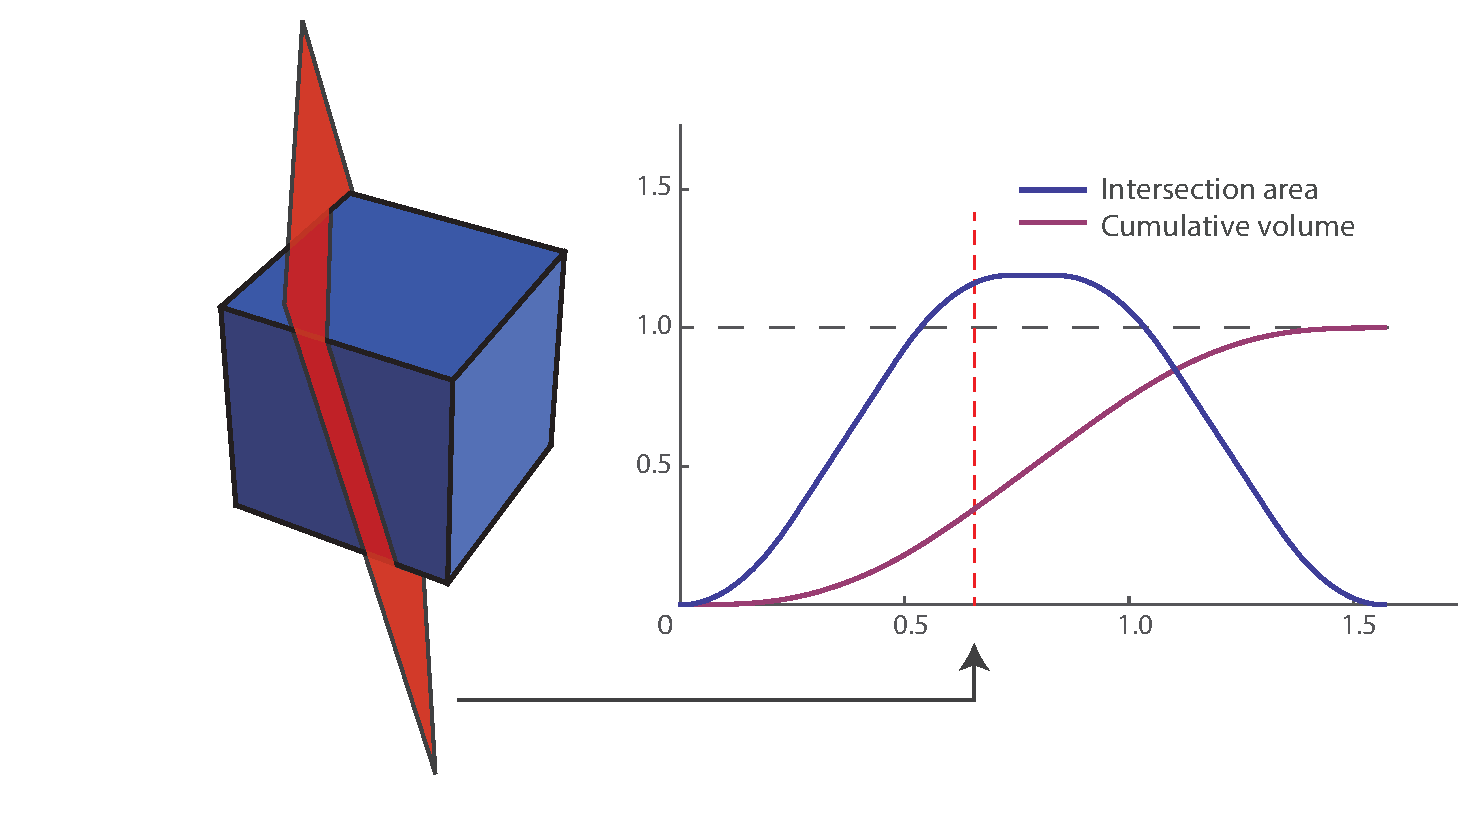
\includegraphics[width=1.\textwidth, clip=true]{./Chapters/03_GLM/./Images/Cube}
	\caption{The plane of arbitrary normal $\vec{n}$ (here $\vec{n}=(n_x, n_y, n_z)=(0.841, 0.480, 0.249)$) divides a unit voxel in two parts (red dashed line). As the plane moves in the direction its the normal, the area of intersection varies, as indicated by the blue curve. The volume within the voxel on the left side of the plane is indicated by the cumulative volume and represented by the purple curve.}
	\label{fig:cube}
\end{figure}
This procedure easily generalises to multiple layers being present in a single voxel, as it corresponds to an intersection with multiple planes. The volumes for the respective layers are hence given by the integral of the intersection area from one plane to the next. The gradient estimate is voxel specific rather than layer specific (i.e. planes are assumed to be parallel) and the same intersection function is used. 

\subsection{The laminar time course}
Once the layer volume distribution is constructed, it can be applied to MRI data. For all given voxels within a region of interest, the voxel signal values represent our measurement data $\mathbf{Y}$. The rows of the design matrix $\mathbf{X}$ give the fractions of the voxel volumes ascribed to the corresponding layer by the layer volume distribution. The layer estimates $\mathbf{\hat{B}}$ can be obtained by regression of $\mathbf{Y}$ against $\mathbf{X}$, given covariance matrix $\mathbf{\Omega}$. In order to obtain a laminar time course from an ROI in fMRI time series, the regression can be performed sequentially for that ROI. Note that the unmixing matrix is independent of the temporal signal, so the regressor calculation needs only to be performed once.

% % % %
\subsection{Similarity to existing methods} 
Hitherto, two main methods of extracting laminar time courses have been used. In the first one, the cortical surface is represented by two triangular meshes, the white matter surface and the pial surface. A laminar profile is then obtained by drawing lines from points (vertices) on one surface to the other. The volume projected onto these lines gives a cortical profile. In computing this projection, the volume has to be sampled by means of some interpolation method. This approach has been used in a number of implementations  \cite{Koopmans2011,Polimeni2010,DeMartino2013}. The second method is a classification of each voxel to be in a given layer based on the single most likely layer per voxel. The signal is subsequently averaged over the region of interest \cite{Siero2011,Olman2012,Maass2014}. Interestingly, all methods can be seen in the light of the same mathematical framework. 

% interpolation
Interpolating a volume at different cortical depths across a part of the cortex effectively creates a weighting for all voxels with respect to the layers. 
The weighting in this procedure is based on a limited set of vertices that form the mesh a weighting matrix. While it is not guaranteed that all voxels in the region of interest are equally represented, one could likely assume that in the limit of an infinite number of lines the result would be similar to our laminar design matrix $\mathbf{X}$. The way in which the average is taken for all lines is then equivalent to a multiplication with the data, normalised with respect to the number of voxels:
\begin{equation}
\hat{\mathbf{B}}_{interpolation}= \mathbf{X^T} \cdot \mathbf{Y} / N. 
\end{equation}
Here $\hat{\mathbf{B}}$, $\mathbf{X}$, and $\mathbf{Y}$ are respectively the estimated layer signals, the weighting matrix, and the voxel signals and have the same dimensions as in Eq.\ref{eq:glm}. $N$ is the number of voxels. We argue that such multiplication with our constructed design matrix is the best-case scenario of performance of the interpolation method.

% classification
Classification of voxels is a more direct attempt to obtain a layer volume distribution, with the property that all entries are binary, with exactly a single 1 in each row. Hence, by definition, the columns are orthogonal, and the average of the multiplication of an orthogonal design and the data is identical to regression of the data onto the same design. Therefore, classification can be viewed as a form of regression, but with a simplified design matrix. 

In the limit of infinite resolution, each voxel would fall into exactly one layer and it can readily be seen that all methods would be rendered equivalent. A similar scenario presents itself when the cortex is exactly aligned with the layering and each layer falls into precisely one voxel. In order to adequately compare all methods and reduce any bias induced by the variety of existing implementations, we here use the identical weighting matrices in the manner as described above. 

%%Add something here to give explicit plan of paper. 
To ascertain the behaviour of all methods, we first test the principles of the method on a simulated cortex of which we know that it behaves according to the equivolume principle. An OLS estimation is used, as there is no (un)correlated noise added to the system. In order to get a more detailed understanding of the behaviour of the method, we used high resolution (post mortem) data. The resolution and the anatomical detail allowed us to get a high number of layers and to assess a longer cortical profile. As the method is likely to be used on human in vivo data, we subsequently assessed anatomical profiles for 11 subjects. We give a detailed account of the influence of the extracted number of layers and we investigate the performance of different FWHMs that can be used for a GLS estimation.
\section{Methods}
% Intro of three methods
The performance of our layer extraction method is assessed by means of three experiments. \change{First, a model cortex with six layers was constructed. The model cortex has physiologically acceptable folding parameters and its layering satisfies equivolume conditions.}{First, we test the principles of the method on a simulated cortex. The model cortex has physiologically acceptable folding parameters and its layering satisfies equivolume conditions. An OLS estimation is used, as there is no (un)correlated noise added to the system.} \change{Secondly, a high-resolution post-mortem sample of the primary visual cortex (V1) was delineated and the cortical profiles were extracted. As V1 shows a particularly strong layer structure, due to the highly myelinated layer IVc (stripe of Gennari), this structure served as a benchmark for testing our method.}{Secondly, to get a detailed understanding of the behaviour of the spatial GLM with a high number of layers, we used high resolution (post mortem) data from the primary visual cortex (V1). V1 shows a particularly strong layer structure due to the highly myelinated layer IVc (stripe of Gennari), such that the comparative performance of the methods could be easily evaluated.}\change{Thirdly, the method was tested on anatomical data using 11 in-vivo data sets to obtain the cortical profile from V1.}{Thirdly, as the method is likely to be used on human in vivo data, we subsequently assessed anatomical profiles for 11 subjects. We give a detailed account of the influence of the extracted number of layers and we investigate the performance of different FWHMs that can be used for a GLS estimation.} All layerings were performed on upsampled data of twice the resolution. As previously described, the best-case scenarios of the other two methods can be easily characterised in the same theoretical framework as our proposed method. Hence, in order to make the cleanest comparison between methods, all extraction methods start from the same layer volume distribution. 
\begin{itemize}
\item The GLM method: The layer volume distribution is used as design matrix and regressed against the voxel signals.
\item The interpolation method: the same design is used, but normalised (division of each element by the sum of its column) and multiplied with the data instead of regressed.
\item The classification method: a regression is used , but the layer presence in the design is redistributed per voxel in a winner-takes-all manner. 
\end{itemize}

\subsection{Model cortex 
\label{sec:Simulation}}
% Why a spring-mass system
In order to most cleanly compare the different methods, we established a gold standard for cortex layering. We simulated a cortex as a spring-mass system, capturing the key properties of the cortex. Most importantly, as mentioned above, the \change{histological}{cytoarchitectonic} layers of the cortex approximately conserve volume ratio over sulci and gyri, which has become known as Bok's principle \cite{Bok1929,Waehnert2014} and is implemented in CBS Tools \cite{Bazin2014}. The intention of the simulation was to generate a layered model cortex that is consistent with the underlying assumptions of the layer extraction methods, rather than to generate a fully physiologically plausible model of the cortex. The equivolume principle leads to the best description of \change{histological}{cytoarchitectonic} layering available to date, but still does not precisely capture the layer locations \cite{Waehnert2016}.

% So what did we simulate?
Six initially equi-distant layers were generated in a two-dimensional piece of cortex that was positively and negatively curved, to simulate gyri and sulci respectively. Note that these layers are not intended to be equivalent to \change{histological}{cytoarchitectonic} layers. The layers started out with unequal volumes but were allowed to evolve until the volumes of all layers were equal, up to a precision of three orders of magnitude smaller than their size. This is illustrated in Figure~\ref{fig:simulation}. A detailed description of the simulation is outlined in Appendix~\ref{sec:Appendix1}.
\begin{figure}[ht]
\centering
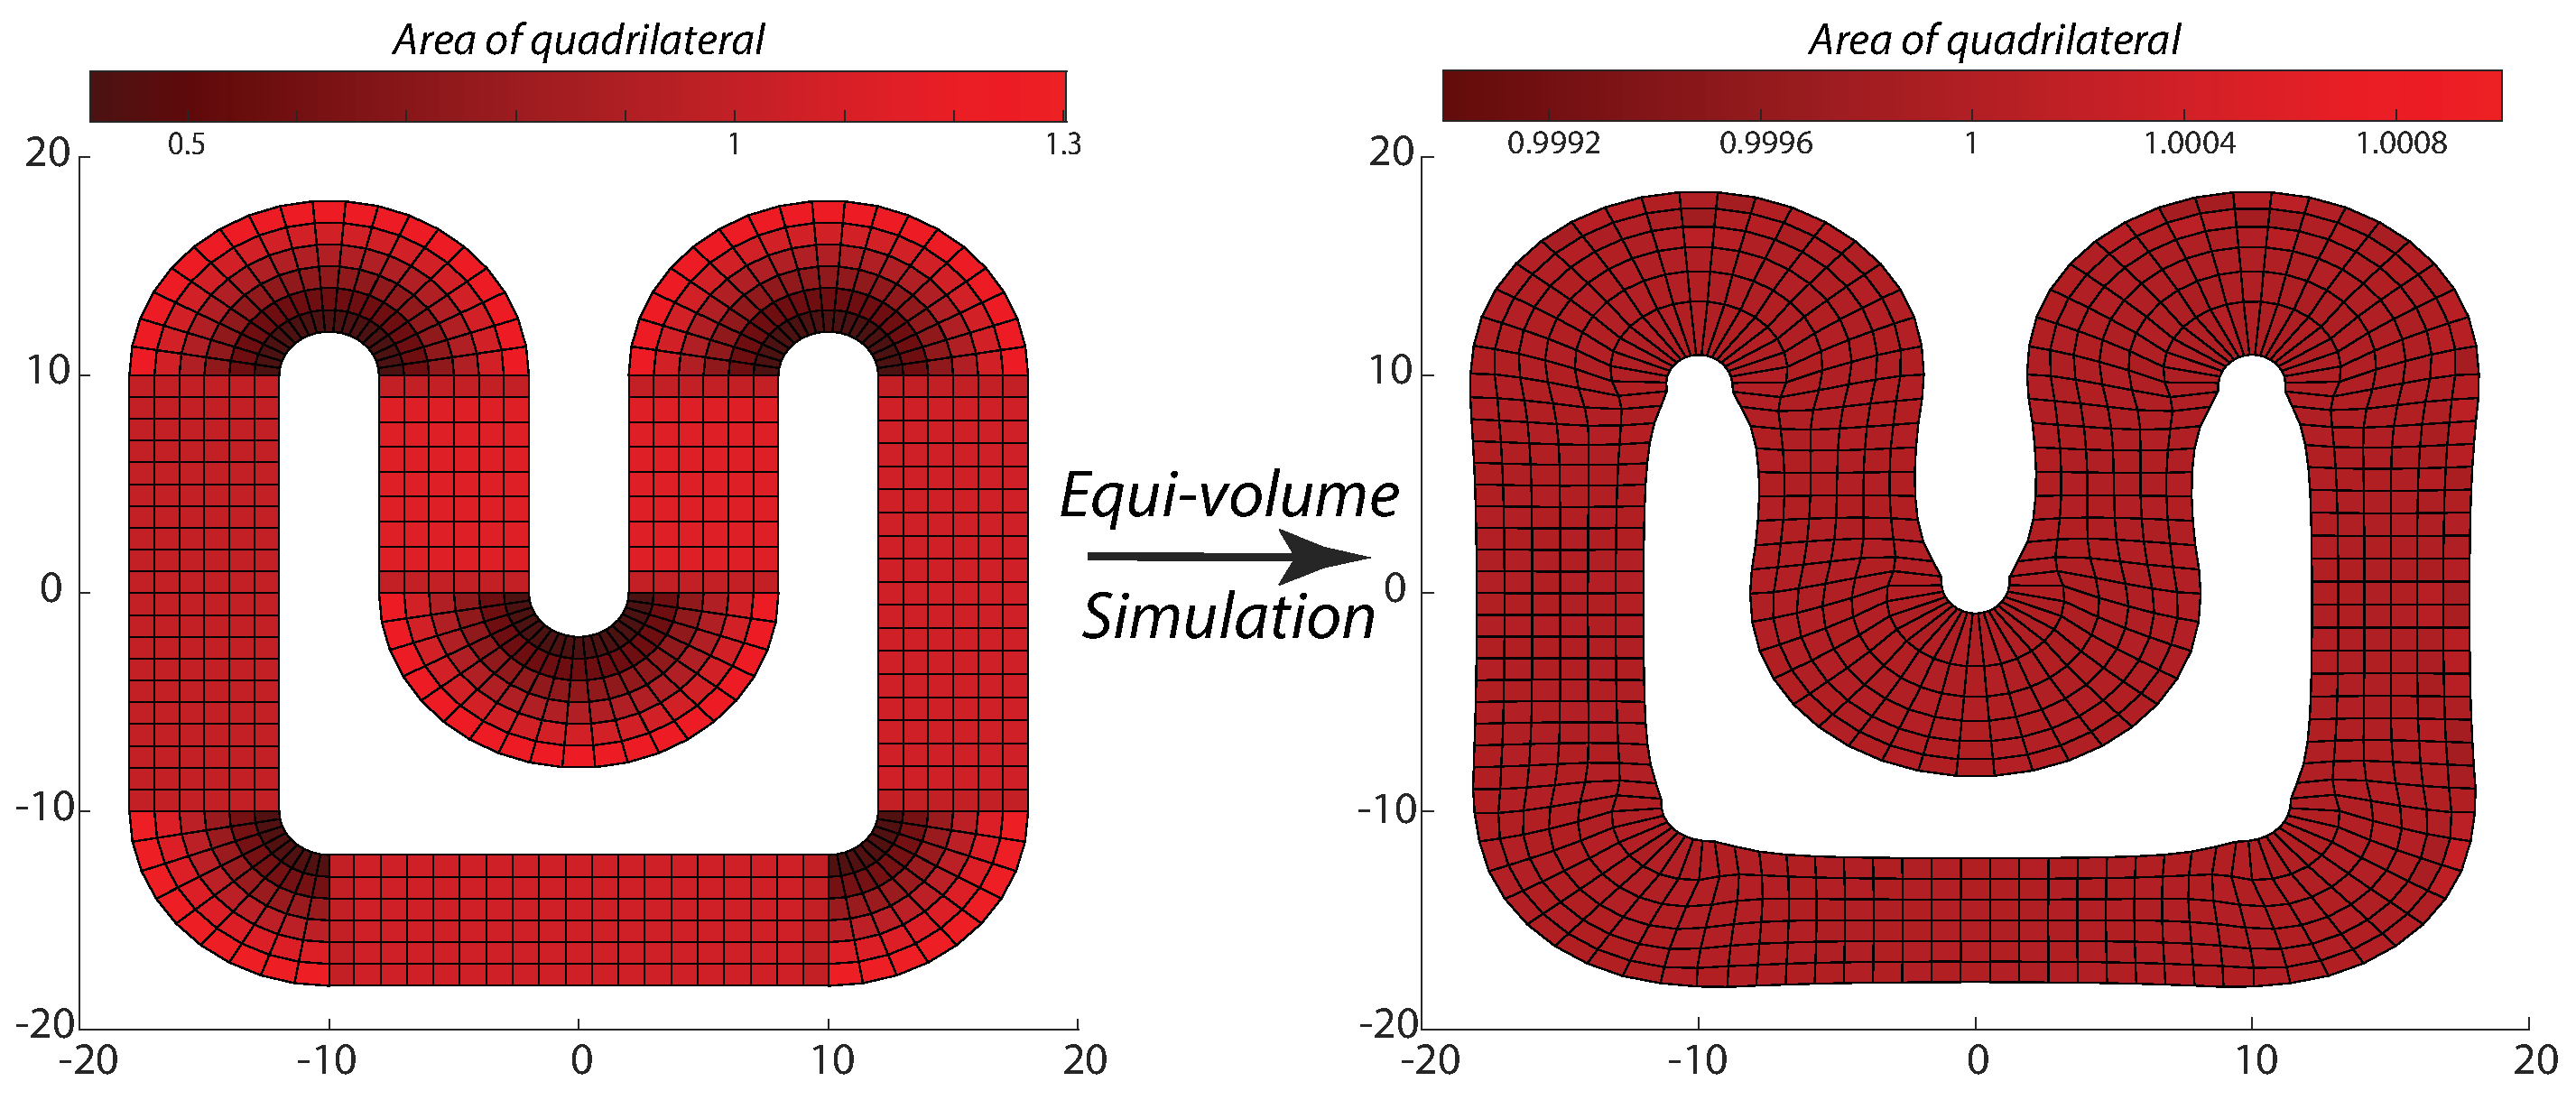
\includegraphics[width=1.\textwidth, clip=true]{./Chapters/03_GLM/./Images/Simulation}
\caption{From an initially equidistant mesh, on the left, we let the points on the mesh rearrange itself in an equivolume manner. The area of a single quadrilateral is indicated by its colour. The resulting mesh, on the right, is rearranged such that all quadrilaterals had unit area ($\pm 10^{-3}$). Note that as a result, the layers start varying in thickness in the inner and outer bends.}
\label{fig:simulation}
\end{figure}

The two-dimensional simulation was first rotated to break alignment with the voxel grid. Next, it was extruded to the third dimension, and resampled to a $64^3$ voxel grid. The simulation covered approximately one voxel per layer. With six layers and an approximate cortical thickness of 3.0 mm \cite{Zilles1990,Fischl2000}, the volume mimicks a resolution of $[0.5$ mm$]^3$. The outer boundaries from the simulation, corresponding to the white matter and pial surfaces, were taken as input for the layering methods. The cortex was divided into six layers and the layering was performed on upsampled data, a factor 2 in each dimension. Treating the simulated layers as a gold standard, the signal leakage between layers can be determined in terms of a spatial point spread function (PSF). The PSF of all methodologies is determined by simulating volumes in which one layer is given the value one; the remainder are set to zero. The extent to which this single layer signal can be retrieved in the correct layer is represented as a PSF. This analysis was performed on a small part of the simulated cortex (ROI shown in Figure~\ref{fig:simulationvolume}) such that positively and negatively curved regions were equally represented. In order to investigate the effect of spatial resolution on the PSF, the simulated data of $[0.5 $mm$]^3$ resolution was downsampled to $[1.0$ mm$]^3$. The same boundaries and the same layering methods and signal extraction procedures were used. No noise was added to the data, so likewise, we did not model any noise covariance in the regression equation and used the ordinary least squares solution.
\begin{figure}[ht]
\centering
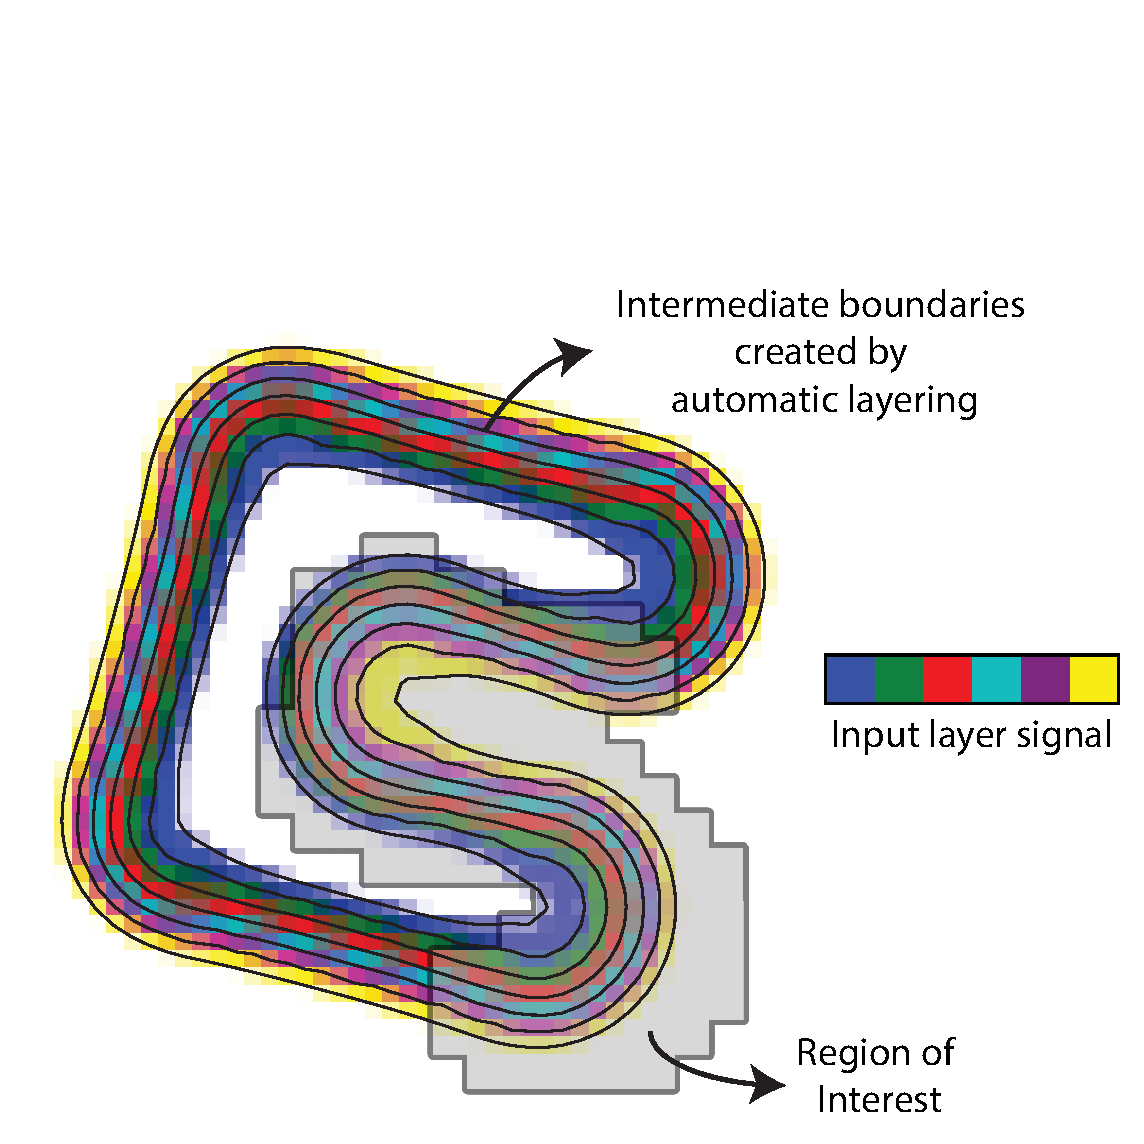
\includegraphics[width=0.7\textwidth, clip=true]{./Chapters/03_GLM/./Images/LayeringSimulation}
\caption{}
\label{fig:simulationvolume}
\end{figure}

\subsection{High-resolution data}
In order to assess the performance of the layer extraction method, we examined a high-resolution post-mortem sample of the visual cortex (V1) of [0.1 mm]$^3$ isotropic resolution. The thickness of this particular region was measured to be between 2 mm and 3 mm. The full experimental setup has been described by Kleinnijenhuis et al. \cite{Kleinnijenhuis2013}. Briefly, prior to MR imaging, samples were fixed (>2 months), soaked in phosphate buffered saline (>72h) and mounted in a syringe with proton-free liquid (~24h). An MGE (multiple gradient-echo) sequence was used with parameters: TR=3.2 s; 7 echoes; TE1=3.9 ms; echo spacing=5 ms; matrix=250x180; FOV=25x18 mm; TA=612 s. The echoes were averaged and bias field corrected.

The aim was to extract anatomically accurate profiles including the stria of Gennari, a myelinated band of nerve fibres running parallel to the surface that is clearly visible in the image. We wanted to investigate the comparative performance of all methods in a real human cortex, but on clean high resolution data. This way, there was a clear image of the true profile, and sufficient detail that should be revealed in the extracted profile. We classified the grey matter by means of thresholding and manually adapted it to ensure accuracy over the entire region of interest. The pial surface and the white matter surface were created based on these segmentations. From these boundaries, the level set was computed and the layering was performed with 20 equivolume layers. 
\remove{This is equivalent to approximately 1 to 1.5 voxels per layer.}
 Three regions of interest were taken, shown in Fig~\ref{fig:exvivovolume}. They varied in curvature and respectively contained 1757, 924, and 1246 voxels \add{and were 2.07 mm, 2.09 mm, and 1.97 mm thick, so this is equivalent to one layer per voxel}. The results were qualitatively compared. 

\subsection{MP2RAGE data}
Lastly, the method was applied to extract profiles from in-vivo data. We examined the cortical profile of the calcarine sulcus in 11 subjects from a T1-weighted MP2RAGE, acquired with a Siemens 7T scanner, with an isotropic resolution of 1.03 mm$^3$, TR/TE/TI1/TI2 = 5000ms/1.89ms/900ms/3200ms, of the calcarine sulcus. The MP2RAGE was chosen for its homogeneous contrast and sharp transition from white to grey matter, such that the leakage effect to neighbouring layers could be investigated. All scans were processed by FreeSurfer \cite{Dale1999} by means of \texttt{recon-all} and the boundaries generated were used in our layer pipeline. We investigated the effect of number of layers by segmenting the volume into 2, 4, 6, and 8 layers. Additionally, we wanted to test the assumption of correlated noise that we proposed in order to use generalised least squares. We compared four different FWHMs for the noise covariance, 0, 1, 2, and 3 mm, where the 0 mm effectively reduces to an ordinary least squares solution. The region of interest was a small portion of the V1 label from the Destrieux atlas that is automatically generated by FreeSurfer \cite{Fischl2004}. It was trimmed to a small part around the calcarine sulcus, because a fundamental assumption of the GLM is that the layer signal estimates are identical across the entire cortex. This cannot be guaranteed over large patches of cortex, especially because it is known that the myelination throughout the visual cortex is variable, e.g. higher around the calcarine sulcus \cite{Bridge2005}. The number of voxels in the ROI was $2009 \pm 494 (\mu \pm \sigma)$ and the average thickness was 3.4 mm $\pm$ 0.3 mm $(\mu \pm \sigma)$. An example for a representative subject is shown in Figure~\ref{fig:invivovolume}. The profiles were extracted on the same volume on which the segmentation and cortical reconstruction were performed, so there was no need for image registration.
\begin{figure}[ht]
\centering
\includegraphics[width=0.8\textwidth, clip=true]{./Chapters/03_GLM/./Images/LayeringInVivo}
\caption{The layering (rainbow colours) and the region of interest (pink) for a representative subject. A small portion of an anatomically defined V1 region was taken in order to investigate the cortical profile in the region.}
\label{fig:invivovolume}
\end{figure}

\subsection*{Data Availability}
All source code for the \change{registration algorithm}{spatial GLM} is freely available at \url{https://github.com/TimVanMourik/OpenFmriAnalysis} under the GPL 3.0 license. The respective modules are also available in Porcupine \url{https://timvanmourik.github.io/Porcupine}, a visual pipeline tool that automatically creates custom analysis scripts \cite{VanMourik2017}. All code to generate the images in this paper are available at the Donders Repository \url{https://webdav.data.donders.ru.nl/dccn/DSC_3015016.05_733}.


\section{Results}
We here show the results of a cortical layering on simulated data, human ex vivo data, and human in vivo data. We compare the extracted laminar signals for three different methods, the GLM, interpolation, and classification approach.

\subsection{Model Cortex}
The three different layer extraction methods were first applied to the modelled cortex, in order to estimate a point spread function of the method in ideal circumstances. The layer profiles of all layers were aligned and averaged \remove{(\texttt{nanmean})} and are shown in Figure~\ref{fig:pointspread} for both resolutions ($[0.5 $ mm$]^3$ and ($[1.0 $ mm$]^3$). The full unaveraged point spread functions are also shown in Supplementary Figure~\ref{fig:pointspreadall} in matrix form. The ideal PSF is a single peak of height one at the origin with no leakage to neighbouring layers.
\begin{figure}[ht]
	\centering
	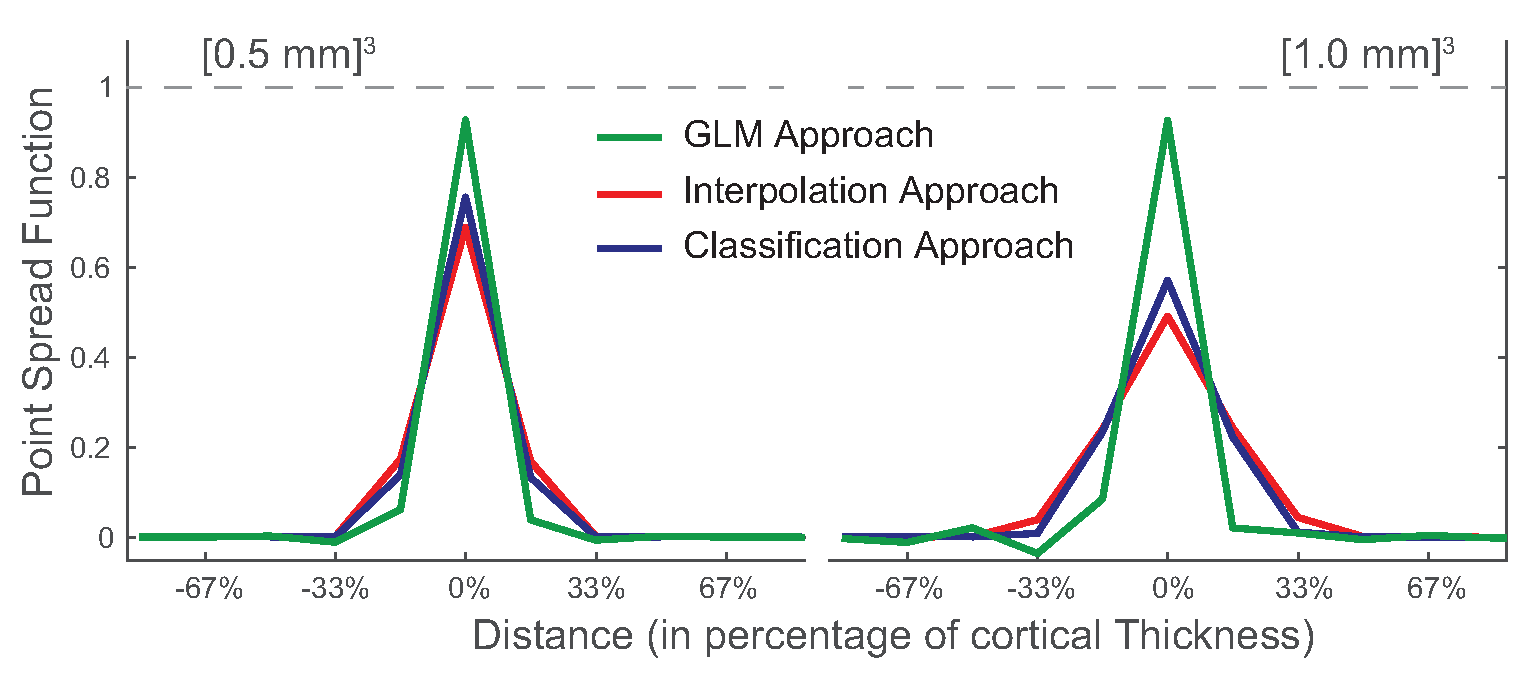
\includegraphics[width=1.\textwidth, clip=true]{./Chapters/03_GLM/./Images/PointSpread}
	\caption{The performance of the three different approaches of obtaining layer signal, represented as a point spread function (PSF) obtained on simulated data. An ideal PSF would be an unit peak at the origin. The results are shown for approximate resolutions of 0.5 mm and 1.0 mm, on the left and right respectively. The GLM approach has a sharper PSF and is able to retrieve more signal, but potentially at the cost of a small undershoot in neighbouring layers.}
	\label{fig:pointspread}
\end{figure}

For the 0.5 mm resolution volume \add{(i.e. one layer per voxel)}, the peak of the distribution for the GLM reaches 92,5\%, which is considerably higher than the 75.4\% for the classification approach and 68,7\% for the interpolation approach. This means that the latter two approaches respectively lose approximately a quarter and a third of the signal to neighbouring layers, as opposed to a only 7.5\% in the GLM approach. For all methods, the leakage is close to symmetrical. The small remaining asymmetries are likely to be related to a small imbalance in proportion of voxels with a positive and negative curvature.

Also for the 1.0 mm scenario, the PSF for the GLM approach is considerably sharper. The GLM approach peaks with 92.4\%, the classification approach with 56.9\%, and the interpolation approach with 49.0\%. As expected, the PSFs for the interpolation and classification approach are less sharp for coarser resolutions. Surprisingly, the GLM approach peaks higher, but this comes at a cost: several undershoots are visible in a sinc-like oscillating pattern. Effectively, this artificially boosts the peak signal by `stealing' it from other layers. \add{The spatial design matrix is more ill-conditioned as the number of layers is double the number of voxels over the thickness of the cortex.}

The same analysis was repeated without including the gradient estimate in the layering, and instead using a cubic polynomial approximation for the partial volume kernel \cite{Koopmans2011}. The resulting PSFs were identical up to 2\% margin, showing that incorporating this extra type of prior knowledge has merely marginal effects on the outcome.

\subsection{High resolution data}
The extracted profile of the high resolution data is shown in Figure~\ref{fig:exvivovolume}, together with an image of the data in which the region of interest is delineated. The structure of the cortex is clearly visible in the extracted profiles. It shows the intensity difference around the stria of Gennari. Additionally, towards the pial surface there is a drop in intensity of which the anatomical origin is unknown. Also note the sharp transition at the pial boundary, quickly dropping to almost zero. The average profiles look like accurate reflections of the ROI, but all methods performs roughly the same. It should be noted, however, that in all regions the GLM shows some oscillating behaviour which is likely to be artifactual to the method. This can easily be related to the sinc-like point spread function that was computed in the simulation. This effectively represents a kernel that is convolved with the true profile and thus shows the same oscillatory behaviour, much related to Gibbs ringing \cite{Gibbs1898}. In particular, the artifacts proliferate at the edges of the cortex, as they scale as a function of the differences between neighbouring layers.
\begin{figure}[ht]
\centering
\includegraphics[width=1.\textwidth, clip=true]{./Chapters/03_GLM/./Images/MichielData}
\caption{The layering, the regions of interest, and the extracted cortical profiles for three regions. While all three methods perform almost identically, there are small oscillations present in the profiles as produced by the GLM. Especially in the top layer, the peak is potentially mistakenly higher than both other methods suggest.}
\label{fig:exvivovolume}
\end{figure}

\subsection{MP2RAGE data}
The cortical profiles of the primary visual cortex for 11 subjects is shown for a variety of methods in Figure~\ref{fig:profileaverage}. First, the three main methods were compared based on the average over subjects. The error bars represent the standard error of the mean. The classification and interpolation approach both show smooth monotonically decreasing profiles for any number of layers. In all case, the GLM method estimates the WM signal to be higher and the CSF signal to be lower than both other methods. This could reflect a lower partial volume leakage to neighbouring layers, but may be indistinguishable from an edge enhancing artifact similar to the ones visible in the previous results. Without a gold standard, this cannot be assessed. In contrast to the two other methods, the GLM starts showing oscillating behaviour when the cortex is divided into more layers. \add{In particular, when the artifacts seem to increase dramatically when the number of layers is higher than the number of voxels.} While the average over subjects is still relatively smooth, the increasing standard errors already suggests higher subject specific differences. This is especially visible in the subject specific profiles (second row of Figure~\ref{fig:profileaverage}). The highly fluctuating individual profiles for 8 cortical layers is unlikely to reflect any true underlying anatomical variation. In general, no method seems to be able to extract anatomical details, such as the stripe of Gennari. Anecdotally, the stripe is visible in some subjects, but it does not survive the anatomical variation in combination with the sensitivity limitations of the layer extraction pipeline.

Lastly, we investigated the assumption of correlated noise in the volume. We varied the \change{FWHM}{correlation length} of an assumed Gaussian noise correlation, performed a generalised least squares regression, and investigated the average profiles. For $L_c= 0$ mm, the solution reduces to an ordinary least squares problem. It can be observed that for a small \change{FWHM}{correlation length} (1 mm), there is only a marginal difference with no correlated noise at all. With a larger \change{FWHM}{correlation length} (2 mm), all profiles become somewhat smoother, but for larger values (3 mm) results start to wildly fluctuate to the extent that they are uninterpretable. It can therefore be concluded that GLS should only be used with extreme care, and that the results with the tested covariance matrices show marginal improvements at best over OLS.
\begin{figure}[ht]
	\centering
	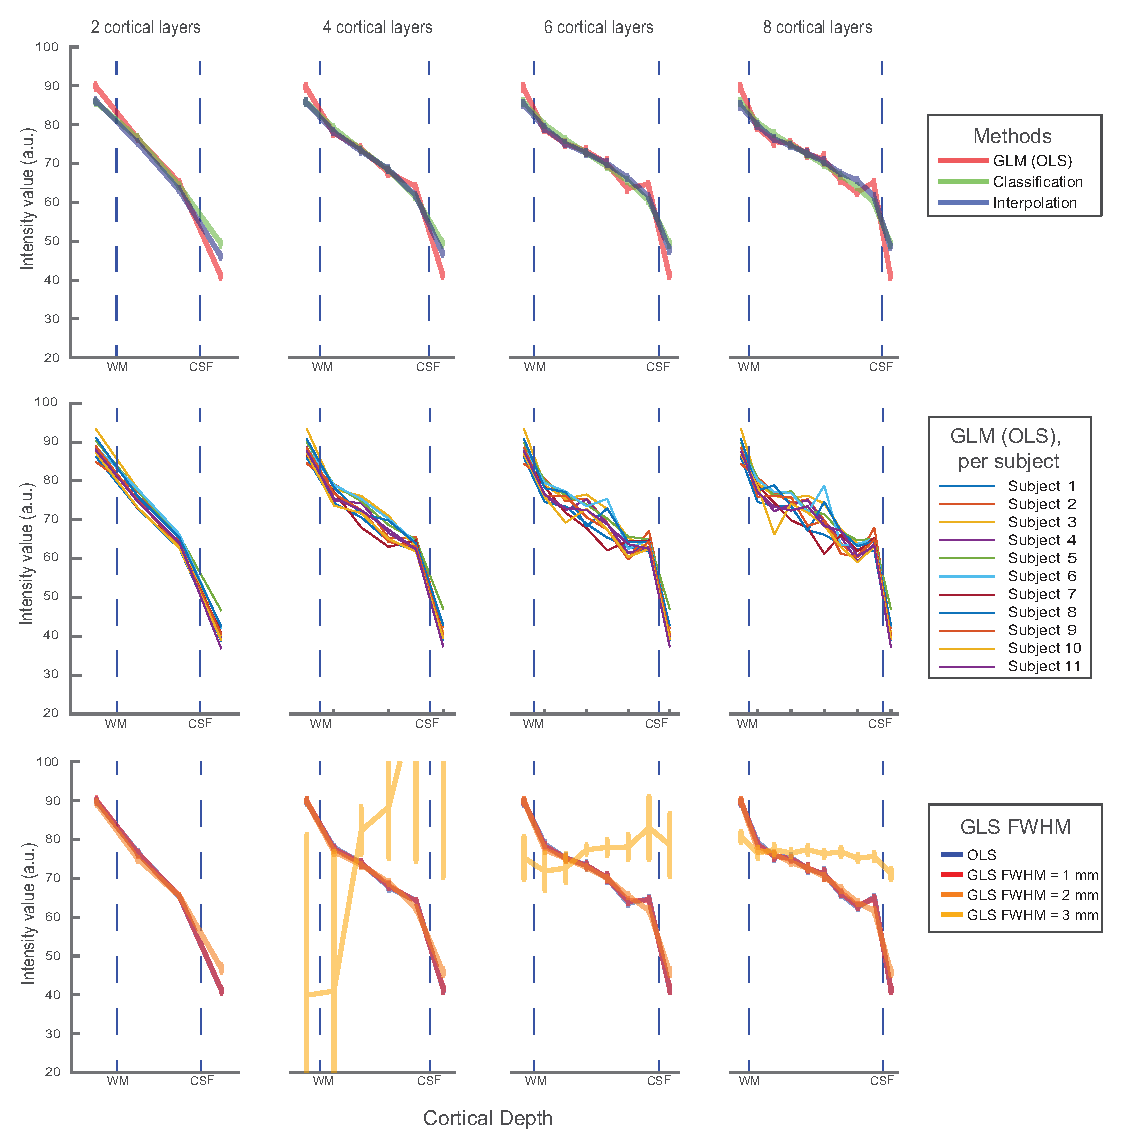
\includegraphics[width=0.9\textwidth, clip=true]{./Chapters/03_GLM/./Images/ProfileComparisons}
	\caption{The obtained profiles for a small piece of the primary visual cortex, based on 11 subjects, for a varying number of layers (columns). In the first row, the three different methods are compared. The second row shows the individual profiles for the GLM method, showing that the solution becomes unstable when higher numbers of layers are used. In the bottom row, different FWHMs are tested in a generalised least squares solution.}
	\label{fig:profileaverage}
\end{figure}

\section{Discussion and Conclusions}
% Conclusion
In this study, we propose a new method to reduce the inherent blurring of laminar profiles of current methods. Instead of interpolating a volume and averaging over a region of interest, we propose to unmix the laminar signals by using a spatial General Linear Model (GLM). In order to further reduce partial volume contamination we propose using the orientation of the voxel with respect to the cortex to better model the layer contributions to each voxel. While this provides an additional type of prior knowledge to incorporate into the layer estimation, the improvements on the layer estimates are marginal. We compute a spatial Point Spread Function (PSF) of existing cortical signal extraction methods on simulated data and explore the benefits and caveats of the spatial GLM when it is performed on human structural MRI data. On simulated data, we show that the GLM clearly outperforms existing methods, especially on a coarser resolution. However, it may be more sensitive to the imperfections of real human MRI data and result in artifacts in the extracted profile, mainly when a high number of layers is used. An initial version of this method has been applied to functional data by Kok et al. \cite{Kok2016} and in \change{Chapter 4 of this thesis}{Van Mourik et al (2018, in prep)} \cite{VanMourik2018a}.

% Assumptions of the GLM
The framework of the GLM is a well described mathematical tool and many principles transfer directly to our proposed spatial application. The core assumption of the GLM (as well as \change{for}{of} existing methods) is that the laminar signals across every layer within the ROI are assumed to be constant. This means that any bias field that stretches through the region of interest may be detrimental to the results. Another important assumption is the normality of errors, either uncorrelated in an ordinary least squares estimation, but potentially correlated for a generalised least squares estimation. This normality is not guaranteed (and sometimes not even expected) in a laminar GLM, due to the many different sources of noise. Apart from thermal noise in the data, important sources can be the presence of e.g. blood vessels that systematically bias some part of the region of interest.
%
At least as important as noise in the data, is noise in the model. Whenever the layer specific design matrix does not match the true underlying structure, (systematic) errors are likely to appear. While the assumed equivolume model for the cortex is the best description to date, it cannot be assumed to be a flawless description of the true cortical layering. \add{Additionally, algorithmic implementations by necessity make numerical approximations that may induce noise as well.} \change{Additionally,}{Correct layering also depends on the quality of the} cortical reconstructions \add{that} may contain errors, especially in regions where the cortex is thin \change{(i.e. visual cortex)}{(i.e. primary visual or somatosensory cortex), highly myelinated (i.e. primary areas),} or regions of reduced signal (e.g. temporal lobe, but highly dependent on acquisition). Related to this, there is a high co-occurence of neighbouring layers in the same voxels, which directly translates into a high covariance between neighbouring layer regressors. In general, covariance between regressors may induce anticorrelations, closely related to the well known anticorrelations found after global signal regression \cite{Uddin2009}. It should therefore come as no surprise that we find the point spread function of the GLM to have sinc-like characteristics and that profiles with many layers (i.e. more heavily correlated regressors) show oscillating patterns.

% Balancedness of design
\change{In the same way that it is important to have a balanced design matrix (over conditions) in a temporal GLM}{It is well known that a temporal design matrix needs to be balanced over conditions. Conditions needs to be represented equally in the model, or otherwise the estimation may be biased towards overrepresented conditions. Similarly}, it is important to have a balanced spatial design. If not, the estimation will be biased towards the overrepresented layer. This has an immediate practical implication: our implementation allows for differing layer thicknesses, which can be useful in order to match the \change{histological}{cytoarchitectonic} layer thickness. But care must be taken, as this may introduce a bias towards the thicker layers as they contribute more to the squared error.
% error bars
We do not provide error margins on our retrieved layer estimates, as the \add{number of }degrees of freedom in our data is not equal to the number of voxels. A valuable course for further research could be a more accurate estimation of the true degrees of freedom in order to get a better handle on the reliability of the extracted layer profiles. 

The main caveat of the GLM method is the potential anticorrelation that is artificially induced in neighbouring layers. This artifact presents itself in space, but also directly translates into lower temporal correlations between neighbouring layers. As a result, one may easily conclude that neighbouring layers are temporally more distinct than is justified. Additionally, this artifact is amplified when the difference between neighbouring layers is large. Unfortunately for fMRI, this is mainly at the white matter boundary and the CSF boundary, and consequently primarily affects the deepest and highest layers. A hypothetical equal activation over the cortex may thus be amplified to appear like deep and top layer activation. If an odd number of layers is chosen, effects from both sides may even amplify to push down every second layer. While an unmixing model alludes to a superresolution potential, we strongly advise against using it as such. Using more than one layer per voxel may compromise the stability of the extracted signals. \add{This is also illustrated by initial use in Huber et al.} \cite{Huber2017} \add{where significant noise enhancement is observed compared to other methods.}

% Future work
An interesting extension of our proposed spatial GLM could be a more seemless integration with a temporal GLM, analogous to the commonly performed first and second level analysis. This spatio-temporal regression is currently performed as a two-stage approach, but could also be combined in the form of a mixture model. This is more powerful due to reduced propagation of errors \cite{Beckmann2003} and would directly yield task-specific laminar results. As we here focus on the validation of the single time point scenario, this is outside the scope of this paper. A different line of improvement could be a more bottom-up approach with a forward modelling perspective of the same problem\add{: a perspective where hypothesised laminar signals is multiplied with the layer model and compared to measured data}. We here took the top-down approach by taking an existing mathematical framework, but experienced \change{that several of the core assumptions of the GLM are not met, resulting in artifacts in the result}{artifacts in the result as a consequence of the model inversion}. Building this up in a different mathematical context may get around these violations of assumptions and provide a formulation that is closer to the problem at hand. Integrating a spatial component into a temporal layer specific hemodynamic forward model \cite{Heinzle2016} could be a interesting starting point.

Hitherto, a mathematical framework has been lacking which has made it difficult to assess certainty \change{values or degrees of freedom}{estimates} of laminar signals, which in turn has made it difficult to apply rigorous statistics. With this work, we hope to provide a contribution to such a framework in the field of laminar (f)MRI, such that it can be conducted on a more routine basis. The main use of this technique is envisioned in fMRI, where better layer extraction will allow a closer examination of layer specific BOLD in functional MRI. This may give new insights regarding feedback and feedforward connectivity of cortical areas. The spatial GLM poses improvements to dealing with the partial volume effect and prevents leakage to neighbouring layers. While there are several caveats of applying the spatial GLM on real data, we show that the performance on simulated data is far better than existing methods. We thus suggest that the price paid for a higher accuracy in ideal data is a higher susceptibility to less than ideal data.

\section{Acknowledgements}
We thank Michiel Kleinnijenhuis for providing the high-resolution data. We would like to thank Daniel Gallichan, Martin Havl\'i\v cek and Ron van den Burg for the helpful discussions. Tim van Mourik acknowledges support by the Spinoza grant [SPI 40-118].
\section{Spring-Mass System}
\label{sec:Appendix1}
\subsection{Introduction}
The cerebral cortex consists of a convoluted surface of gyri and sulci. There are accurate models for the gyrification of the cortex as a whole \cite{Tallinen2014} and there is a description of how the layers within the cortex behave \cite{Bok1929}: the volume ratio between layers is equal for an arbitrarily curved pieced of cerebral cortex. This is what has become known as the Bok-principle. Here we describe how to simulate data for a two dimensional system that obeys Bok's principle by means of a spring-mass system. A spring-mass system was chosen, because it is independent of the algorithms by means of which we estimate curvature in the volume. This makes it ideal benchmark data for the methods presented in the body of this paper.

\subsection{Spring-Mass System}
The cortex is modelled by means of a spring mass system. This is an approximation of the cortex consisting of quadrilaterals. Each quadrilateral consists of four edges and four vertices, which are the springs and masses respectively. The collection of springs and masses that form quadrilaterals will henceforth be referred to as the system.

The system has total energy $U$. In the present simulation only a single contribution to the energy is considered, related to the area of each quadrilateral. More generally, other contributions could be taken into account, for example relating to the length of each edge:
\begin{equation}
U=U_{area}+U_{edge}+...
\end{equation}
We are looking for the case where the energy is minimised, as this is when the system has come to rest and all quadrilaterals have reached an equilibrium area. Note that only the vertices are displaced in the first instance; the edges and quadrilaterals are formed as a consequence. The energy decreases by moving the vertices in the direction of the net force applied to them. The force $\vec{F}_n$ on vertex $n$ is minus the derivative of $U$ with respect to the position $\vec{r}_n$ of that vertex: 
\begin{equation}
\vec{F}_n= -\nabla_n U.
\label{Forces}
\end{equation}

% \subsubsection{Area force}
A quadrilateral $Q_i$ is defined to be the space enclosed by four vertices in two dimensions  $\vec{u_i}$, $\vec{v_i}$, $\vec{w_i}$ and $\vec{k_i}$, shown in Figure~\ref{Tetrahedron}.
\begin{figure}[ht]
\begin{center}
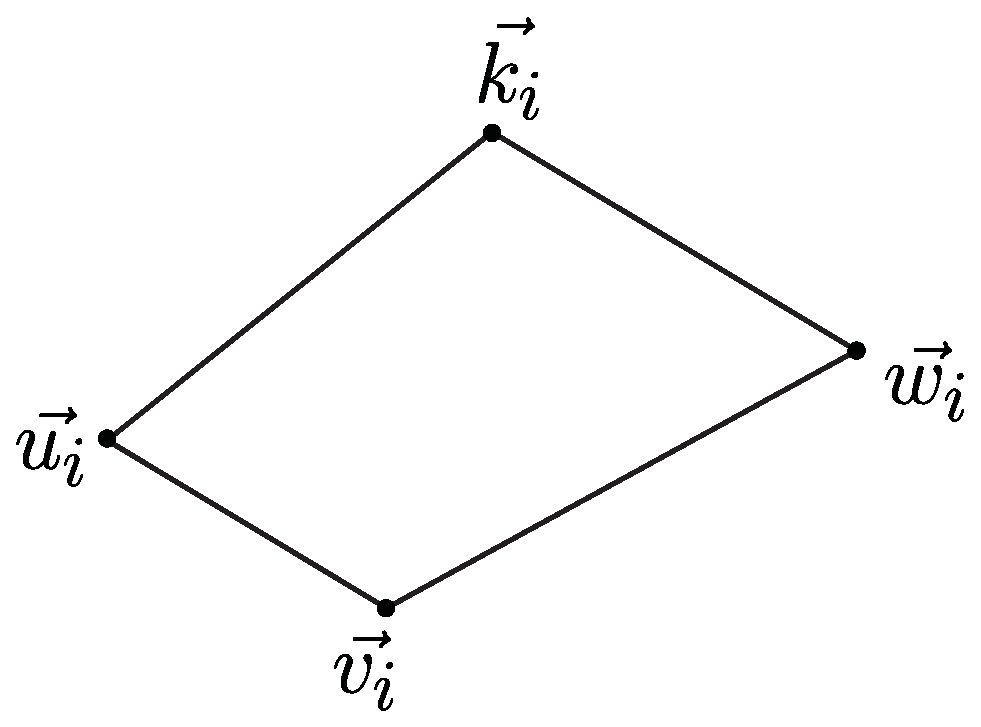
\includegraphics[width=0.33\textwidth, clip=true]{./Chapters/03_GLM/./Images/Quadrilateral} 
\caption{Quadrilateral $Q_i$, consisting of vertices $\vec{u_i}$, $\vec{v_i}$, $\vec{w_i}$ and $\vec{k_i}$.}
\label{Tetrahedron}
\end{center}
\end{figure}
Its area $A_i$ is a scalar function depending on the vertices of the quadrilateral,~$A_i=A_i(\vec{u}_i, \vec{v}_i, \vec{w}_i, \vec{k}_i)$: 
\begin{eqnarray}
A_i&=&\frac{1}{2}
[\left( u_{i,y} v_{i,x} - u_{i,x} v_{i,y} \right) + \left( v_{i,y} w_{i,x} - v_{i,x} w_{i,y} \right) + \textellipsis \\
& & \left( w_{i,y} k_{i,x} - w_{i,x} k_{i,y} \right) + \left( k_{i,y} u_{i,x} - k_{i,x} u_{i,y} \right) ]
\label{areaQ}
\end{eqnarray}
The vertices $\vec{u_i}$, $\vec{v_i}$, $\vec{w_i}$ and $\vec{k_i}$ are chosen such that $A_i > 0$.

Let $Q = \{Q_1, Q_2, Q_3, ...\}$ be the set of all quadrilaterals. The energy of the system is
\begin{equation}
U=U_{area}=\sum\limits_{Q_i\in Q}U_i
\end{equation}
where $U_i$ is the energy of quadrilateral $Q_i$
\begin{equation}
U_i=\frac{1}{2}k_A \left(A_i-A_0\right)^2
\end{equation}
such that the quadrilateral energy is a function of the difference between the actual area $A_i$ and the equilibrium area $A_0$. 

Subsequently, the gradient is computed for the energy stored in the system:
\begin{equation}
\nabla_n U_{area}=\nabla_n \sum\limits_{Q_i\in \vec{Q}} U_i=\sum\limits_{Q_i\in Q} \nabla_n U_i.
\end{equation}
The gradient of a single quadrilateral energy term takes the form:
\begin{equation}
\nabla_n U_{i} = \nabla_n \frac{1}{2}k_A\left(A_i-A_0\right)^2 = k_A \left(A_i-A_0\right) \nabla_n A_i.
\label{EnergyLaplacian}
\end{equation}
Note that $\nabla_n U_{i}$ can be non-zero only if vertex $n$ belongs to $Q_n$, i.e. if $\vec{r}_n$ is one of the vertices $\vec{u_i}$, $\vec{v_i}$, $\vec{w_i}$ or $\vec{k_i}$. To be explicit, let $\vec{r}_n = \vec{u_i}$. In two dimensions $\nabla_n A_i = ( \frac{\partial A_i}{\partial u_{i,x}}, \frac{\partial A_i}{\partial u_{i,y}} )$. The two components follow immediately from \ref{areaQ}:
\begin{eqnarray}
\frac{\partial A_i}{\partial u_{i,x}}&=&
\frac{1}{2} \left( k_{i,y} - v_{i,y} \right),
\nonumber \\
\frac{\partial A_i}{\partial u_{i,y}}
&=&
\frac{1}{2} \left( v_{i,x} - k_{i,x} \right).
\label{uglypartialderivatives}
\end{eqnarray}

Combining equations~\ref{Forces}, \ref{EnergyLaplacian} and \ref{uglypartialderivatives}, the resulting force on vertex $n$ due to the preservation of volume is
\begin{equation}
\vec{F}_n = \sum\limits_{Q_i \ni n} -\frac{1}{2}k_A (A_0-A_i) \left( k_{i,y} - v_{i,y}, v_{i,x} - k_{i,x}\right).
\end{equation}
Here the summation is over the quadrilaterals $Q_i$ that contain vertex $n$, and $\vec{k}_i$ and $\vec{v}_i$ are the neighbours of $\vec{r}_n$ in $Q_i$. The vertex will come to rest if $A_i=A_0$, and the strength of the force can be adjusted by parameter $k_A$. All forces are additive.


This was implemented in C\texttt{++} as a stand-alone application. The program reads in a mesh and evolves the vertices until the system comes to rest. 

\section{Orientation dependent partial volume distribution}
\label{sec:Appendix2}
In order to find out how different laminae are distributed over voxels, it is important to know the orientation and location of the surface with respect to the voxels. Here we analytically describe an algorithm to solve this problem.

The intersection of a laminar surface and a voxel is approximated by the intersection of a cuboid and a plane that are arbitrarily positioned and oriented with respect to each other.

The voxel grid is given by three primitive lattice vectors $\{\vec{a_1}, \vec{a_2}, \vec{a_3}\}$, having the orientation and length of the voxel edges. The lattice vectors are usually but not necessarily oriented along the cardinal axes. For a cubic voxel grid with edge length $L$ the primitive lattice vectors are $\{L \hat{x}, L \hat{y}$ and $L \hat{z}\}$.
A voxel can be indexed with three integers $m_i$. The centre position $\vec{m}$ of the voxel is 
\begin{equation}
 \vec{m}=\sum_{i=1}^{3}m_i \vec{a_i}
\end{equation}
and the 8 corner positions $\vec{c}$ of the voxel are
 \begin{equation}
 \vec{c}=\sum_{i=1}^{3}\left(m_i \pm \frac{1}{2} \right) \vec{a_i}.
\end{equation}
The voxel volume is $V=\vec{a_1}\cdot \left( \vec{a_2} \times \vec{a_3}\right)$.

A plane can be defined by a vector $\vec{N}$. The plane is perpendicular to $\vec{N}$ and has distance $1/\|\vec{N}\|$ to the origin. The plane is given by all points $\vec{r}$ satisfying
\begin{equation}
 \vec{r} \cdot \vec{N}=1.
\end{equation}
It is useful to express $\vec{N}$ in terms of reciprocal lattice vectors $\vec{b_i}$:
\begin{equation}
 \vec{N}=\sum_{i=1}^{3}N_i\vec{b_i}.
\label{eq:rn=1}
\end{equation}
The reciprocal basis vector $\vec{b_1}$ is defined as $\vec{b_1}=\vec{a_2} \times \vec{a_3} / V$, $\vec{b_2}$ and $\vec{b_3}$ are obtained by cyclic permutation. For a cubic voxel grid, the  reciprocal basis vectors are $\vec{b_1}=\hat{x}/L$, $\vec{b_2}=\hat{y}/L$ and $\vec{b_3}=\hat{z}/L$. By construction $\vec{a_i}$ and $\vec{b_i}$ are orthonormal to each other
\begin{equation}
\vec{a_i} \cdot \vec{b_j} = \delta_{ij}.
\end{equation}

Points on the four edges of voxel $\vec{m}$ in the direction $\vec{a_1}$ are of the form
\begin{equation}
\vec{r}=(m_1 + \lambda_1)  \vec{a_1}+\sum_{i=2}^{3}(m_i\pm\frac{1}{2}) \vec{a_i}, \hspace{5pt}  |\lambda_1 | \le \frac {1}{2}.
\end{equation}
In view of \ref{eq:rn=1} the four possible 
intersection points of $\vec{N}$ with the edges parallel to $\vec{a_1}$ are given by the four $\lambda_1$ of the form
\begin{equation}
\lambda_1 N_1 = 1 -\sum_{i=1}^{3}m_i N_i \pm\frac{1}{2} N_2 \pm\frac{1}{2} N_3.
\end{equation}
Analogously the possible intersection points with the edges parallel to $\vec{a_2}$ and $\vec{a_3}$ are given by four $\lambda_2$ and $\lambda_3$ values respectively. Of the 12 possible intersection points, those with $|\lambda_i | \le \frac {1}{2}$ give the actual (at most 6) intersection points. The area of the polygon connecting the intersection points can be readily computed, as well as the volume on either side of the plane. 

At this point we have expressions for the intersection point that are independent of the choice of the voxel edge vectors $\vec{a_i}$. Explicit expressions can be obtained for the intersection points and intersection area. To be explicit, consider the intersection of a plane, moving with a given orientation, i.e. $\vec{N} = t \vec{n}$ where $t$ takes arbitrary real values and $\vec{n}$ stays constant. A finite intersection is only found for the range of $t$ values between the maximum and
minimum value of $1/[\sum_{i=1}^{3} (m_i \pm\frac{1}{2}) n_i]$.
%why moving, there is no reason to consider a plane moving through a cube
\newpage

\section{Supplementary Figures}
%\section*{Figures}
% Supplementary
\renewcommand{\thefigure}{S\arabic{figure}}
\setcounter{figure}{0}
\begin{figure}[ht]
\centering
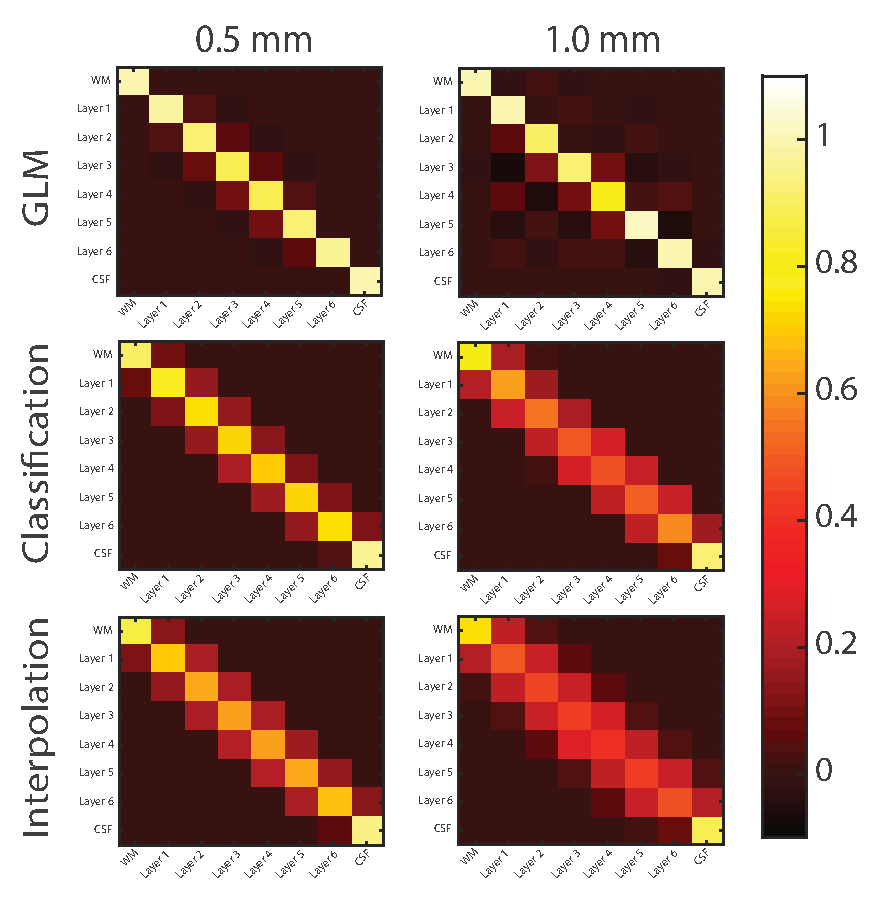
\includegraphics[width=0.9\textwidth, clip=true]{./Chapters/03_GLM/./Images/PointSpreadMatrices}
\caption{The point spread functions of all layers for both resolutions and both methods. An ideal point spread function would look like an identity matrix. This is approached more by the GLM method for both resolutions.}
\label{fig:pointspreadall}
\end{figure}


\chapter{Investigation of layer specific BOLD during visual attention in the human visual cortex}
\chaptermark{Layers in Spatial Attention}
\label{ch:attention}

\textcolor{gray}{{Tim van Mourik$^{1,*}$}, Peter J Koopmans$^{2,*}$, Lauren J Bains$^{1}$, David G Norris$^{1,2,\dagger}$, Janneke FM Jehee$^{1,\dagger}$\\
$^{1}$Radboud University Nijmegen, Donders Institute for Brain, Cognition and Behaviour, Nijmegen, The Netherlands \\
$^{3}$Erwin L. Hahn Institute for Magnetic Resonance Imaging, University Duisburg-Essen, Essen, Germany}\\

$^*$ 		{These authors contributed equally to this work}
$^\dagger$  {These authors contributed equally to this work}

%----------------------------------------------------------------------------------------
%	ABSTRACT
%----------------------------------------------------------------------------------------
\linespread{1.5}
\newpage
\section*{Abstract}
It is well-known that directing spatial attention towards a particular stimulus enhances cortical responses at corresponding regions in cortex. How attention modulates the laminar response profile within the attended region, however, remains unclear. In this paper, we use high field (7T) fMRI to investigate the effects of attention on laminar activity profiles in areas V1-V3; both when a stimulus was presented to the observer, and in the absence of visual stimulation. Replicating previous findings, we find robust increases in the overall BOLD response for attended regions in cortex, both with and without visual stimulation. Interestingly, when analyzing the BOLD response across the individual layers in visual cortex, we observed no evidence for laminar-specific differentiation with attention. We offer several potential explanations for these results, including theoretical, methodological and technical reasons.
\newpage
%----------------------------------------------------------------------------------------
\section{Introduction}
Directing visual attention to a location in the visual field typically improves behavioral sensitivity to stimuli presented at that location \cite{Posner1980,Lee1997,Yeshurun1998,Carrasco2004,Baldassi2005,Ling2009}. It is well known that these attentional benefits in behavior are accompanied by increases in BOLD response in early visual areas (e.g. \cite{Brefczynski1999,Gandhi1999,Kastner1999}), but how top-down processes modulate cortical responses at the laminar level remains unknown.

It is known from anatomical studies that the human cerebral cortex can be subdivided into histological layers with different cell types. The cytoarchitectonic structure varies across the brain and forms the basis of the Brodmann atlas, but almost all brain areas have six different histological layers \cite{Brodmann1909}. Although the precise function of each cortical layer remains unclear, their connectivity profile suggests a division in terms of bottom-up and top-down processing \cite{Felleman1991}. Specifically, Layer IV and to a lesser extent Layer V/VI are commonly associated with receiving feedforward drive from Layer III of lower cortical areas or from the thalamus \cite{Jones1998,Constantinople2013}. Layers I-II and VI, in contrast, are typically implicated in receiving downward information flow (feedback), which often originates from layer V \cite{Alitto2003}. Interestingly, this bottom-up versus top-down connectivity profile of each of the layers is to some degree paralleled in functional data. That is, from neurophysiological and neuroimaging work, it is known that various visual stimuli and tasks can exert differential effects on the various layers \cite{Maier2010,Xing2012,Self2013,VelezFort2014, OHerron2016}. Intracranial work in monkeys, for instance, shows that for selective attention and working memory (two functions that are commonly associated with top-down processes), current source density is increased in deep and superficial compared to middle layers in primary visual cortex \cite{VanKerkoerle2017}. Similar layer specific patterns have been shown in animal functional MRI. For instance, whisker stimulation led to an increase in BOLD response in Layer IV of rat barrel cortex, before such an enhancement was observed in any of the other layers, suggesting that layer IV was the first to receive feed forward drive from lower-level areas \cite{Yu2014}. In contrast, subsequent corticocortical connections in the same task appeared to activate Layers II-III and V in the motor cortex and contralateral barrel cortex before this affected any of the other layers, suggesting that these layers were the first to receive feedback signals. To what extent these results generalize to human cortex, however, remains to be investigated.

Recent advancements in fMRI have made it possible to also investigate the functional role of cortical layers in humans (e.g. \cite{Polimeni2010,Maass2014,Kok2016}). The human in vivo resolution with fMRI has increased to submillimetre voxel size. The thickness of the cerebral cortex varies between 1 and 4.5 millimetres \cite{Zilles1990,Fischl2000}, suggesting sufficient resolution to characterise activity across the individual layers. Indeed, some evidence suggests that human cortical activation can be measured with fMRI on a layer specific basis \cite{ Kok2016, Muckli2015}. For example, illusory contours, which are commonly associated with top-down processes, appear to activate the deep layers more than any of the other layers In area V1 \cite{Kok2016}, and some findings suggest that also specific activation of the middle layers can be measured with fMRI in human primary visual cortex \cite{Koopmans2010}.

While some neurophysiological evidence suggests a differential involvement of the cortical layers in top-down attention \cite{Nandy2017}, the effects of attention on the different layers in human visual cortex has remained unclear. Here, we examine with fMRI the potential influence of spatial attention on BOLD activity in the deep, middle and superficial layers in human visual areas V1, V2, and V3. Participants directed their attention to a cued location, and performed an attention-demanding task using an orientation stimulus that was shown at this location, while an unattended grating appeared at a different location of equal eccentricity. On some of the trials, subjects directed their attention to the cued location in anticipation of the stimulus, but no stimulus appeared at this location. Interestingly, although we observed a reliable increase of the overall BOLD response with attention across all layers, both with and without a stimulus present, we observed no differences in activation level between the layers due to attention. We provide several reasons for these surprising findings in the Discussion.

\section{Methods}
\subsection{Participants}
Nineteen healthy adults (aged 22-27, eight female), with normal or corrected-to-normal vision, participated in this study. All participants provided written informed consent in accordance with the guidelines of the local ethics committee. Two subjects were excluded from analysis; one subject was excluded due to insufficient (chance-level) performance on the attention task, and another due to weak retinotopic maps. The remaining data from 17 subjects were analyzed.

\subsection{Experimental design and stimuli}
Observers viewed the visual display through a mirror mounted on the head coil. Visual stimuli were generated by a Macbook Pro computer running MATLAB and Psychophysics Toolbox software \cite{Brainard1997,Pelli1997} and displayed on a rear-projection screen using a luminance-calibrated EIKI projector (resolution 1,024 X 768 pixels, refresh rate 60 Hz).

Participants were required to maintain fixation on a central bull's eye target (radius: 0.25\textdegree) throughout each experimental run. Each run consisted of an initial fixation period (3000 ms) followed by 32 stimulus trials (average duration: 4.7 seconds). Trials were separated by inter-trial intervals of variable duration (1000-2500 ms, uniformly distributed across trials). Each trial started with the presentation of a central attention cue (800 ms). This was followed by a delay period of variable duration (0-5000 ms; drawn from an exponential distribution to ensure a constant hazard rate), after which the two orientation stimuli appeared on the screen (500 ms). The orientation stimuli were followed by a response window (1300 ms), in which the fixation target turned orange.

Stimuli were two counterphasing sinusoidal gratings of independent orientation (\textasciitilde 45\textdegree~or \textasciitilde 135\textdegree; size: 7\textdegree; spatial frequency: 1 cycle per \textdegree; randomized spatial phase; contrast: 50\%; contrast decreased linearly to 0 towards the edge of the stimulus over the last degree), centered at 5\textdegree~to the left and right of fixation. We used a compound white/black cue consisting of two dots (dot size 0.25\textdegree) that straddled the fixation point (0.8\textdegree~to the left and right of fixation) to indicate with 100\% validity which of the two gratings should be attended \cite{Jehee2011}). Subjects were instructed to attend to the same side of fixation as either the white or black dot in the compound cue.

Participants were instructed to detect a small clockwise or counterclockwise rotation in the orientation of the grating at the attended location with respect to a base orientation at 45\textdegree~or 135\textdegree. The size of rotation offset was adjusted with an adaptive staircase procedure using QUEST \cite{Watson1983}, such that participants detected approximately 80\% of the offsets correctly. An overview of the experiment is shown in Fig.~\ref{fig:experiment}.

All but one participants completed 18 stimulus runs. The remaining participant completed 12 runs due to equipment failure.

Retinotopic maps of visual cortex were acquired in a separate scan session at a 3T scanner using conventional retinotopic mapping procedures \cite{Sereno1995,DeYoe1996,Engel1997}. 
\begin{figure}[!ht]
\centering
\includegraphics[width=1.0\textwidth, clip=true]{./Chapters/04_Attention/Images/Experiment}
\caption{Stimuli and experimental procedure. Example of a trial sequence from the experiment. Subjects fixated a central bull's eye target while gratings of independent orientation ($\pm$ 45\textdegree) appeared in each hemifield. A compound black/white cue indicated whether subjects should attend to the left or right stimuli; in this example, the white circle indicates `attend right.' Subjects had to discriminate near-threshold changes in orientation of the attended grating with respect to the closest diagonal. In one-third of trials, no stimuli appeared at either location. Red circles depict the attended location and were not present in the actual display.}
\label{fig:experiment}
\end{figure}

\subsection{MR data acquisition}
Functional images were acquired on a Magnetom Siemens 7T scanner with a 32-channel head coil (Nova Medical, Wilmington, USA) combined with dielectric pads \cite{Teeuwisse2012}, using a $T_2^*$-weigthed 3D gradient-echo EPI sequence \cite{Poser2010} (TR/TE/$\alpha$=3060 ms/20 ms/14\textdegree, 72 slices oriented orthogonally to the calcarine sulcus, voxel size [0.8 mm]$^3$, FOV: [192 mm]$^2 $, GRAPPA factor 8).

Gradient maximum amplitude was 40 mT/m (in practice, however, this maximum wasn't reached), the minimum gradient rise time was 200 $\mu$s, and the maximum slew rate was 200 T/m/s. Shimming was performed using the standard Siemens shimming procedure for 7T. There were 18 runs of 72 $\pm$ 4 volumes. As the lengths of the events and the inter trial interval were of unequal length, there was a small variation in the number of volumes per run.

Finger pulse was recorded using a pulse oximeter affixed to the index finger of the left hand. Respiration was measured using a respiration belt placed around the participant's abdomen.

Anatomical images were acquired using an MP2RAGE sequence \cite{Marques2010} [0.75 mm]$^3$, yielding two inversion contrasts (TR/TE/TI1/TI2 = 5000 ms/1.89 ms/900 ms/3200 m).

In a separate session prior to the main experiment, a retinotopy session was conducted at a Siemens 3T Magnetom Trio scanner. A high-resolution T$_1$-weighted anatomical scan was acquired (MPRAGE, FOV 256 $\times$ 256, 1 mm isotropic voxels) at the start of the session. Functional images were subsequently collected using T$_2^*$-weighted gradient echo EPI, in 30 slices oriented perpendicular to the calcarine sulcus (TR/TE/$\alpha$ = 2000 ms/30 ms/90\textdegree, FOV = 64 $\times$ 64, [2.2 mm]$^3$ isotropic resolution).


\subsection{Functional MRI preprocessing}
\subsubsection{Data preprocessing}
\label{sec:dataProcessing}
Data were corrected for subject motion using SPM with the mean functional volume across time as a reference \cite{Friston1995}. Residual motion-induced fluctuations in the BOLD signal were removed through linear regression, based on the alignment parameters of SPM. Scanner drifts were corrected via linear regression with high-pass filter regressors to filter out frequencies below 1/64 Hz. Pulsating signals as a result of the respiratory and cardiac cycle were removed as follows. The cardiac/respiratory peaks were automatically detected from the physiological recordings using in-house interactive peak-detection software, and manually corrected where needed. With a custom MATLAB implementation of RETROICOR \cite{Glover2000}, fifth order Fourier regressors were constructed for heart rate and respiration and subsequently removed from the functional images via linear regression. A small part (10\% of respiratory measurements, and 18\% of heart rate measurements) was of insufficient quality and could not be used in this analysis. Functional data for these time frames were used in the main analysis but uncorrected for cardiac and respiratory noise.

The functional and anatomical scans were brought to the same space by registering the anatomical surface from the retinotopy session to the mean functional volume using boundary based registration (BBR), implemented in FreeSurfer's \texttt{bbregister} \cite{Greve2009}. All registration results were inspected and manually refined when necessary. Where needed, registration was improved by an additional pass of BBR using an in-house MATLAB implementation. Local distortions in EPI due to field inhomogeneity were corrected by means of recursive boundary registration \cite{VanMourikISMRM2014}, which recursively applies BBR to small portions of the cortical surface to correct topology locally by means of optimizing the grey-white matter contrast along the surface.

Because of temporal changes in magnetic field inhomogeneities, local topology slightly changed over the course of the entire session. For this reason, the 18 functional runs obtained for each subject were first divided in three groups of each 6 contiguous runs, and then each group was pre-processed separately.  Time courses were subsequently concatenated before entering the main analyses.


\subsubsection{Regions of Interest}
Regions of interest (areas V1, V2, V3) were defined on the reconstructed cortical surface using standard retinotopic mapping procedures \cite{Sereno1995,DeYoe1996,Engel1997}. After identifying areas V1-V3, data were smoothed along the reconstructed cortical surface with a Gaussian kernel (FWHM: 4 mm). The smoothed version of the data was only used in region of interest selection, and not in the main analysis. In each area, we then selected the 600 vertices that responded most strongly to the stimulus (shown on the cortical surface in Supplementary Figure~\ref{SM5}). The selected vertices were resampled from the cortical surface back to subject space by means of FreeSurfer's \texttt{label2vol}. T-values of selected voxels ($\mu \pm \sigma$) were V1: $T=2,989 \pm 0.854$, V2: $T=2.317 \pm 0.689$ and V3: $T=2.117 \pm 0.713$). Note that the selection of voxels based on visual activation per se is orthogonal to the analysis of interest, which addresses the effects of attention on individual layers in cortex. Control analyses verified that our results were not strongly affected by the number of vertices selected for subsequent analysis (See Supplementary Figures).

\subsection{Cortical profile extraction}
Layer specific signals were obtained by means of a layer specific spatial General Linear Model (GLM) as proposed by \cite{VanMourikISMRM2015} and briefly described in \cite{Kok2016}. Specifically, we applied the level set method \cite{Sethian1999} on the reconstructed cortical surface \cite{Dale1999} to create a cortical layering of three equivolume layers, following the procedures described in \cite{Waehnert2014}. The gradient and the curvature of the cortex were defined as a function of Laplacian streamlines in the grey matter as this more naturally follows the structure of cortical columns \cite{Leprince2015}. Partial volume inaccuracies were adjusted for by explicitly taking into account the orientation of the voxel with respect to the cortex \cite{VanMourikISMRM2015}. This procedure enabled us to divide the gray matter in three equivolume cortical layers, which amounts to roughly one voxel per layer. We additionally defined a volume on either side of these three cortical layers to capture signals for white matter and cerebrospinal fluid. On the basis of  these definitions, we then created a laminar (spatial) design matrix. By regressing this design matrix against the functional data within an ROI, we obtained laminar time courses. In the regression, we used generalised least squares to account for spatial covariance in the noise. The voxel-to-voxel covariance matrix was defined based on Gaussian noise spread (FWHM 1.41 mm) between neighbouring voxels. 

\subsection{Statistical Analyses}
Temporal linear regression was used to compare between the experimental conditions. Regressors were created as follows. The stimuli appeared during the stimulus window on 2/3rds of trials, which were modeled with a single regressor (stimulus \emph{on}). The remaining stimulus windows were also modeled with a regressor (stimulus \emph{off}). In addition, attention could either be directed to the \emph{left} or \emph{right} visual field; these conditions were each modeled with a regressor. We so obtained four regressors for each of the conditions of interest. To remove any potential influence from the anticipation period, i.e. before stimulus presentation, we additionally included separate regressors for each of these four factors during the anticipation window. We used a canonical HRF (parameters: time-to-peak-parameter: 5 second) to model the fMRI responses. To verify the appropriateness of this function, a finite impulse response (FIR) analysis \cite{Josephs1997} was performed using the data from four pilot subjects (not included in the current study). Based on this pilot data set, temporal or dispersion derivatives were not included into the statistical model. The baseline signal of each run was captured by adding a regressor column of ones for each run separately. As described above (Sec.~\ref{sec:dataProcessing}), the data were pre-processed by means of nuisance regression. This was performed by adding the nuisance regressors to the design matrix, effectively adjusting for the statistical loss in degrees of freedom as a result of nuisance regression. The reference of one percent signal change was the height of a peak of a two-second-long isolated event \cite{Mumford2007}.

The temporal regression was performed on the previously extracted layer-specific time courses. The obtained parameter estimates were divided by their baseline estimates, in order to convert them to percent signal change. The values in percent signal were compared at the group level by means of ANOVAs and t-tests as appropriate. As the experiment was left-right symmetric and we found no differences between hemispheres in the analyses of interest, the hemispheres were treated as two measurements per participant.

\subsection{Code availability}
All functions for laminar analysis that are mentioned here are available on \url{https://github.com/TimVanMourik/OpenFmriAnalysis}. Custom analysis scripts are available on request. The analysis scripts were made with Porcupine pipeline software available on \url{http://timvanmourik.github.io/Porcupine} \cite{VanMourik2017}.



\section{Results}
Subjects generally performed well at the orientation discrimination task. The mean orientation discrimination threshold across participants was 6.6\textdegree, and behavioral performance was quite stable across runs.

\subsection{Spatial attention increases fMRI response amplitudes}
First, we determined whether directing attention to a spatial location led to stronger overall responses in the visual cortex. Regions of interest consisted of voxels that were significantly activated by the stimulus in all layers of areas V1, V2, and V3 (see Methods). We compared the amplitude of the BOLD response with and without attention, for trials in which a stimulus was presented and those in which no stimulus appeared (see Fig.~\ref{fig:roiresults}). Data were analyzed using a general linear model with area, attention (attended vs. unattended), and stimulus (present vs. absent) as factors (see Methods). We first focused on the effects of attention per se. Attention significantly enhanced the BOLD response at the attended location in areas V1-V3 (effect of attention, F(1, 16) = 43.4, p = 6.36$\cdot10^{-6}$), with a trending increase in attention-based activity for higher-level areas (interaction between attention and area, F(2, 32) = 2.63, p = 0.088). The mean effect sizes (in percent signal change) were 0.41\%, 0.64\% and 0.59\% for V1, V2, and V3 respectively, and slightly stronger to those reported before \cite{Murray2008,Jehee2011}. Next, we investigated whether the effects of attention depended on the presence of a visual stimulus. Specifically, we compared attentional effects between trials in which observers were expecting a stimulus but none was presented, and trials in which the stimulus did appear on the screen. Replicating previous reports \cite{Kastner1999}, the effect of attention in areas V1-V3 was not significantly different in the absence compared to presence of visual stimulation (two-way interaction between and attention and stimulus, F(1, 16) = 0.26, p = 0.585), with no reliable change across areas (three-way interaction between stimulus, attention and area, F(2, 32) = 0.026, p = 0.901). Thus, attending to a spatial location enhances the BOLD response at that location, even in the absence of visual stimulation.
\begin{figure}[!ht]
\centering
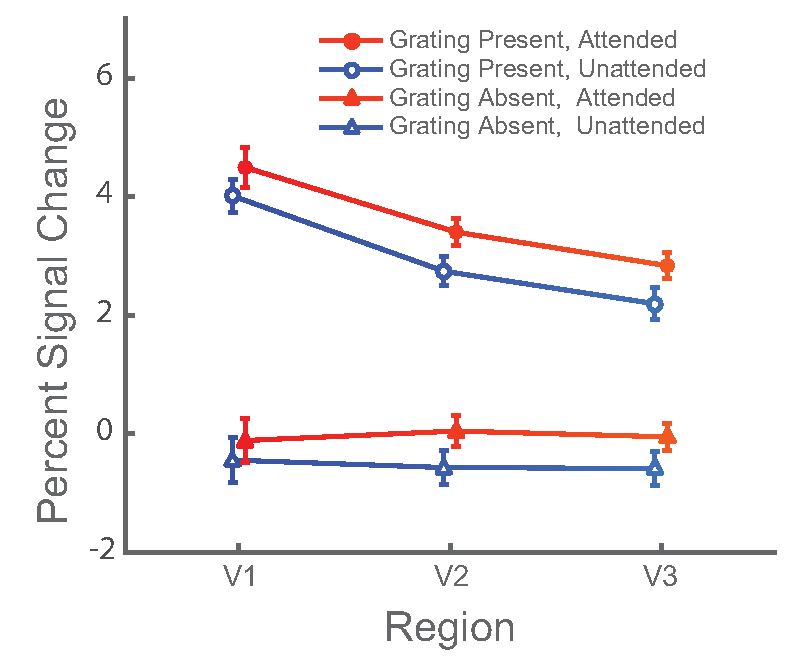
\includegraphics[width=0.8\textwidth, clip=true]{./Chapters/04_Attention/Images/RoiResults}
\caption{Amplitude of the BOLD response for attended and unattended regions in areas V1-V3. Red lines indicate the attended condition, blue the unattended. The top lines (circles) show the response when a grating was presented, the bottom lines (triangles) when no grating was presented, at the attended or unattended location. Response amplitudes were significantly higher for attended than unattended locations and stimuli. Error bars indicate $\pm$1 SEM.}
\label{fig:roiresults}
\end{figure}

\subsection{Spatial attention increases responses across the layers}
Next, we asked whether attention led to changes in the pattern of activity across cortical layers in these areas. We used a spatial general linear model (see methods) to first characterize activity in each of three distinct cortical layers. Data were subsequently analyzed using a temporal general linear model with attention, stimulus, area, and layer as factors (see Methods). Consistent with previous studies \cite{Koopmans2010,Polimeni2010}, we found a general increase in BOLD response from white matter to pial surface (see Fig~\ref{fig:layerresults}, overall effect of layer, F(2, 32) = 12.5, p = 9.85$\cdot10^{-5}$). This increase in BOLD response with decreasing distance to the pial surface was reliably larger in the presence of a stimulus (two-way interaction between layer and stimulus, F(2, 32) = 61.1, p = 1.00$\cdot10^{-11}$), and was significantly different between the three areas (three-way interaction between layer, stimulus, area: F(4, 64) = 3.33, p = 0.015; post hoc analyses revealed a trending larger effect for area V1 compared to V2 (T(16) = 2.11, p = 0.051), and a larger effect for area V2 compared to areas V3 (T(16) = 3.37, p = 0.0039). This tendency of the BOLD response to increase from lower layers to higher layers should be interpreted with caution, however, as blood flows from the gray-white matter boundary towards the pial surface. Hence, any change in BOLD response that arises in layers V-VI will automatically affect the BOLD response in downstream layers. This accumulation of signal may also result in a larger slope of activation through the layers for larger effects with equal laminar activation, thus explaining the greater layer by stimulus interaction in earlier visual regions. In contrast to the layer-specific increase in BOLD signal when presenting a stimulus, we found no significant change in the effects of spatial attention across the layers (two-way interaction between layer and attention, F(2, 32) = 2.33, p = 0.114). This may reflect equal activation of all layers, or a rather shallow slope as a result of low attentional effect. Next, we determined whether the layer-specific increase in BOLD signal with attention was distinct from the observed stimulus-based effects. The attention-based increase in activity was indeed reliably different from stimulus-driven changes in layer response (post hoc comparison between layer by stimulus effect and layer by attention effect; T(16) = 4.94, p = 1.47$\cdot10^{-4}$). However, this effect should be interpreted with caution, as the strength of the layer responses is tightly coupled to the strength of the main effects. In addition, there was no reliable difference between the effects of attention versus stimulus between any of the three layers (three-way interaction between layer, stimulus and attention, F(2, 32) = 1.69, p = 0.200). Control analyses established that these results were not strongly affected by the number of voxels included in the analyses (Supplementary Figures~\ref{fig:layerresults300}-\ref{fig:layerresults900}), nor by the number of layers analyzed (Supplementary Figure~\ref{fig:layerresults4layers}). In addition, these results did not qualitatively change when layer activation profiles were defined using volume interpolation (Supplementary Figure~\ref{fig:layerresultsinterp}). Moreover, combining the anticipation (i.e., time frame prior to when a stimulus could appear, see Figure~\ref{fig:experiment}) and stimulus windows in the analyses did not reliably affect any of these results (Supplementary Figure~\ref{fig:layerresultsplusattention}). Thus, while the overall effects on BOLD activity of both visual stimuli and attention were rather robust and similar to previously reported values for visual cortex \cite{Kastner1999,Jehee2011, Koopmans2010}, no differential pattern of activity was observed between these two processes across the visual cortical layers.
\begin{figure}[!ht]
\centering
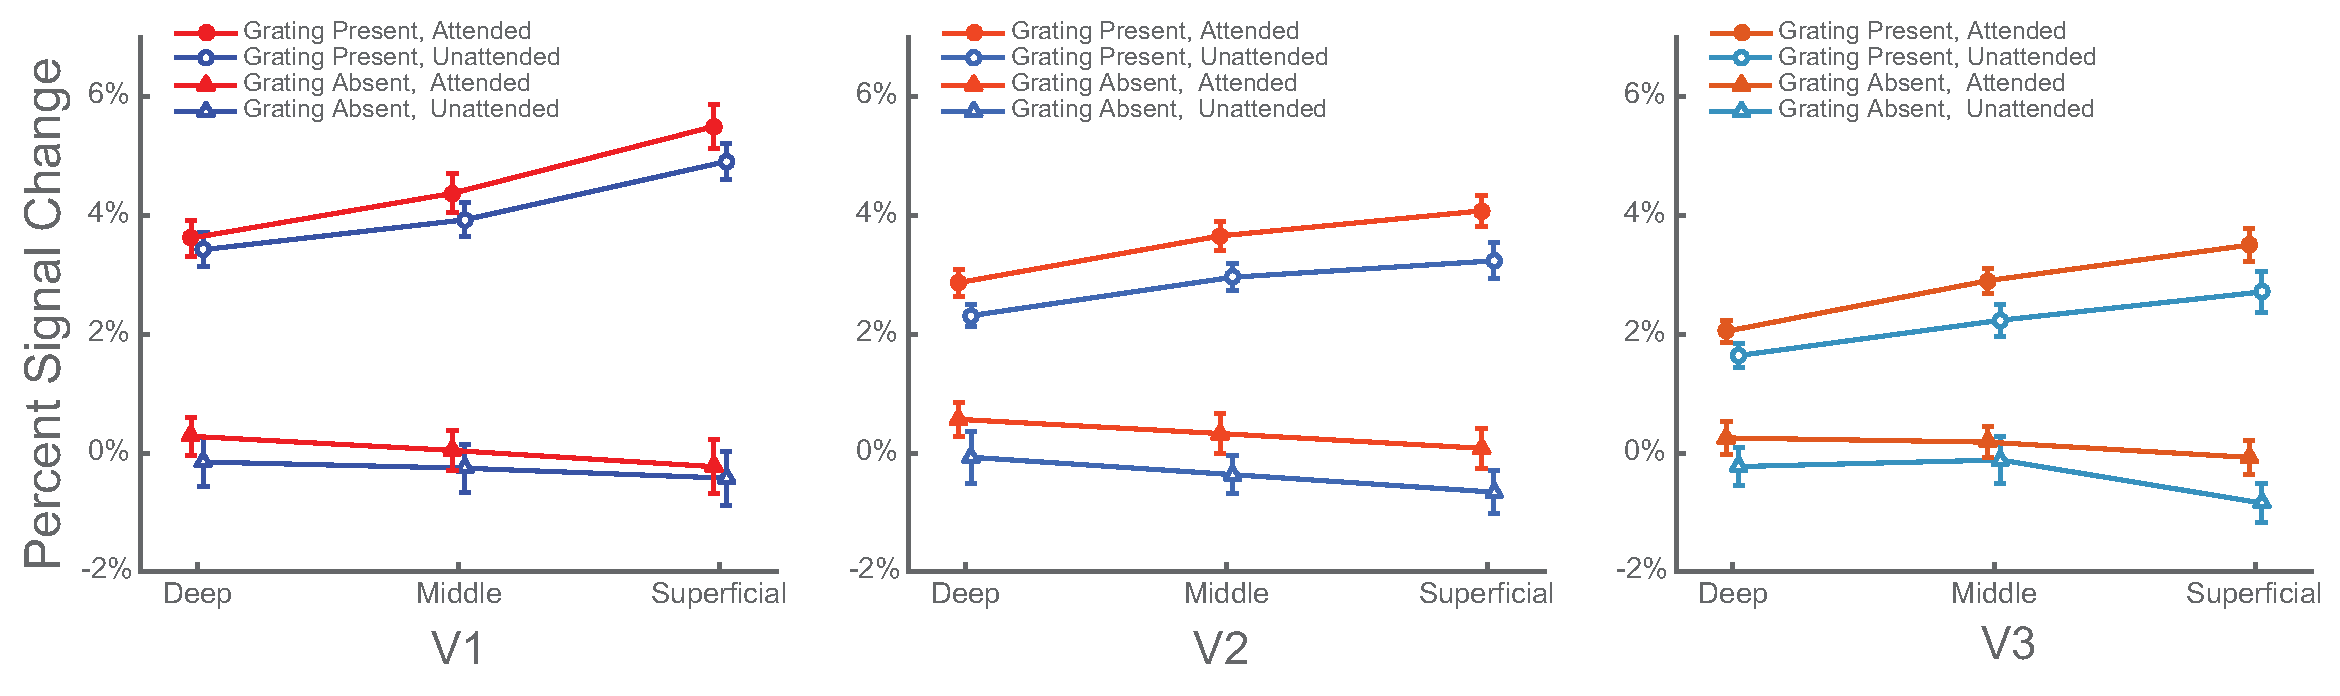
\includegraphics[width=0.8\textwidth, clip=true]{./Chapters/04_Attention/Images/LayerResults}
\caption{Layer-specific amplitude of the BOLD response in the experiment in areas V1-V3. Circles indicate when a grating was presented, squares depict when no grating was presented, at either the attended (red) or unattended (blue) location. When a stimulus was presented, activation reliably increased towards the pial surface. Attention significantly enhanced the BOLD response across all layers. Error bars indicate $\pm$1 SEM.}
\label{fig:layerresults}
\end{figure}




\section{Discussion}
This study investigated the effects of spatial attention on the BOLD signal measured from individual layers in early visual cortex. Focusing first on the overall amplitude of the BOLD response in all layers combined, we found that attending to a stimulus reliably and substantially increased the BOLD signal in early visual areas, both when a stimulus was presented to the observer and in the absence of physical stimulation (cf. \cite{Kastner1999,Murray2008,Li2008}). Moreover, and much in line with earlier results on layer-specific activation patterns in visual cortex (\cite{Polimeni2010,Koopmans2010}), we observed a general increase in activation towards the superficial layers - one that is commonly explained by gradient echo being more susceptible to the draining veins on the pial surface. Interestingly, and much to our surprise, we observed no differential activity in the individual layers when comparing between top-down (attention-driven) and bottom-up (stimulus-driven) activity - a finding that stands in notable contrast to previous observations \cite{Kok2016}. We identify several potential reasons for this absence of layer specific differentiation that we outline and discuss below.
	
One possibility is that our data are simply insufficiently robust for showing a significant difference in activity across depth between the two conditions. It is well known that the BOLD signal includes multiple sources of noise related to both MRI scanner and participant, and this holds especially true for signals recorded at the sub-millimeter scale. For example, at a resolution this high, even the smallest movement of the participant may cause additional blurring of the data, with potentially detrimental effects on the signal-to-noise ratio. For this reason, we collected data from 17 participants - a sample size much larger than typical in attention-based fMRI studies at standard spatial resolution (cf. N=4-6 in\cite{Kastner1999,Kamitani2005,Jehee2011}), and it is even in the larger range for layer-based fMRI studies at high resolution (cf. N=6 in \cite{Polimeni2010}, N=4 in \cite{Muckli2015}, N=10 in \cite{Kok2016}). To minimize the effects of various sources of noise, we took great care in measuring and removing physiological artifacts, and further improved existing layer extraction techniques by developing a novel spatial general linear model that separates laminar signal from different layers instead of sampling a mixed interpolation of the layers. Additionally, we ensured that similar results were obtained using more conventional layer-extraction procedures. Indeed, the combined success of these procedures is well illustrated by the effect sizes observed in the current study for both stimulus presentation (4.5\%, 3.3\%, 2.8\% in V1, V2 and V3) and attention (0.41\%, 0.64\%, 0.59\% in V1, V2 and V3), which are comparable or higher to those reported in previous publications \cite{Murray2008,Jehee2011}. There are, however, some differences in experimental design between our study and previous laminar investigations that could potentially account for the incongruity in results. Because we were interested in the degree to which top-down processes could be dissociated from feed forward stimulation with fMRI, we directly contrasted between these two conditions in our analyses. Previous studies, on the other hand, have focused on top-down activity in isolation (e.g. \cite{Muckli2015, Kok2016}), or used multi-voxel pattern analyses - rather than overall BOLD amplitude, to compare between conditions \cite{Muckli2015}. \cite{Kok2016}, for example, directly compared between the overall activation levels in individual cortical layers, and found a significant difference in BOLD activity due to recurrent signals that were evoked by an illusory stimulus. It will be interesting for future studies to address the degree to which these experimental factors can account for the disagreement in results between our and previous work.

An alternative explanation for the incongruity in results could lie in attention itself, which may be mediated by mechanisms distinct from previously investigated processes. That is, previous work using high-resolution fMRI focused not on spatial attention, but rather on figure-ground segregation \cite{Kok2016} and other non-classical receptive field effects in cortex \cite{Muckli2015}. It is conceivable that these modulatory processes operate on the individual cortical layers in a manner dissimilar from the attentional mechanisms studied here. It is known from primate studies, for example, that attention increases the response gain of neurons in visual cortex \cite{Treue1999,MartinezTrujillo2004} - such an increase in attentional gain could lead to general enhancements in neural activity irrespective of cortical layer, as we have observed here.
	
Regardless of the potential reasons for the disparity between current and previous results, we believe our study presents an important message to a field that is currently in its nascent stages of development. We hope that the results and procedures detailed here will help move the field forward and resolve which experimental parameters are paramount, and which are not, to detecting differential activity between individual layers in human visual cortex with high-resolution fMRI.

\section{Author contributions}
PJK and JFMJ designed the experiment. TvM and LJB collected the data. TvM and DGN developed the laminar analysis techniques. TvM and JFMJ analysed the data. TvM, DGN, and JFMJ wrote the paper. 

\section{Acknowledgements} 
Tim van Mourik acknowledges support by the Spinoza grant [SPI 40-118].
\section{Supplementary Materials}
\setcounter{figure}{0}
\begin{figure}[!ht]
\centering
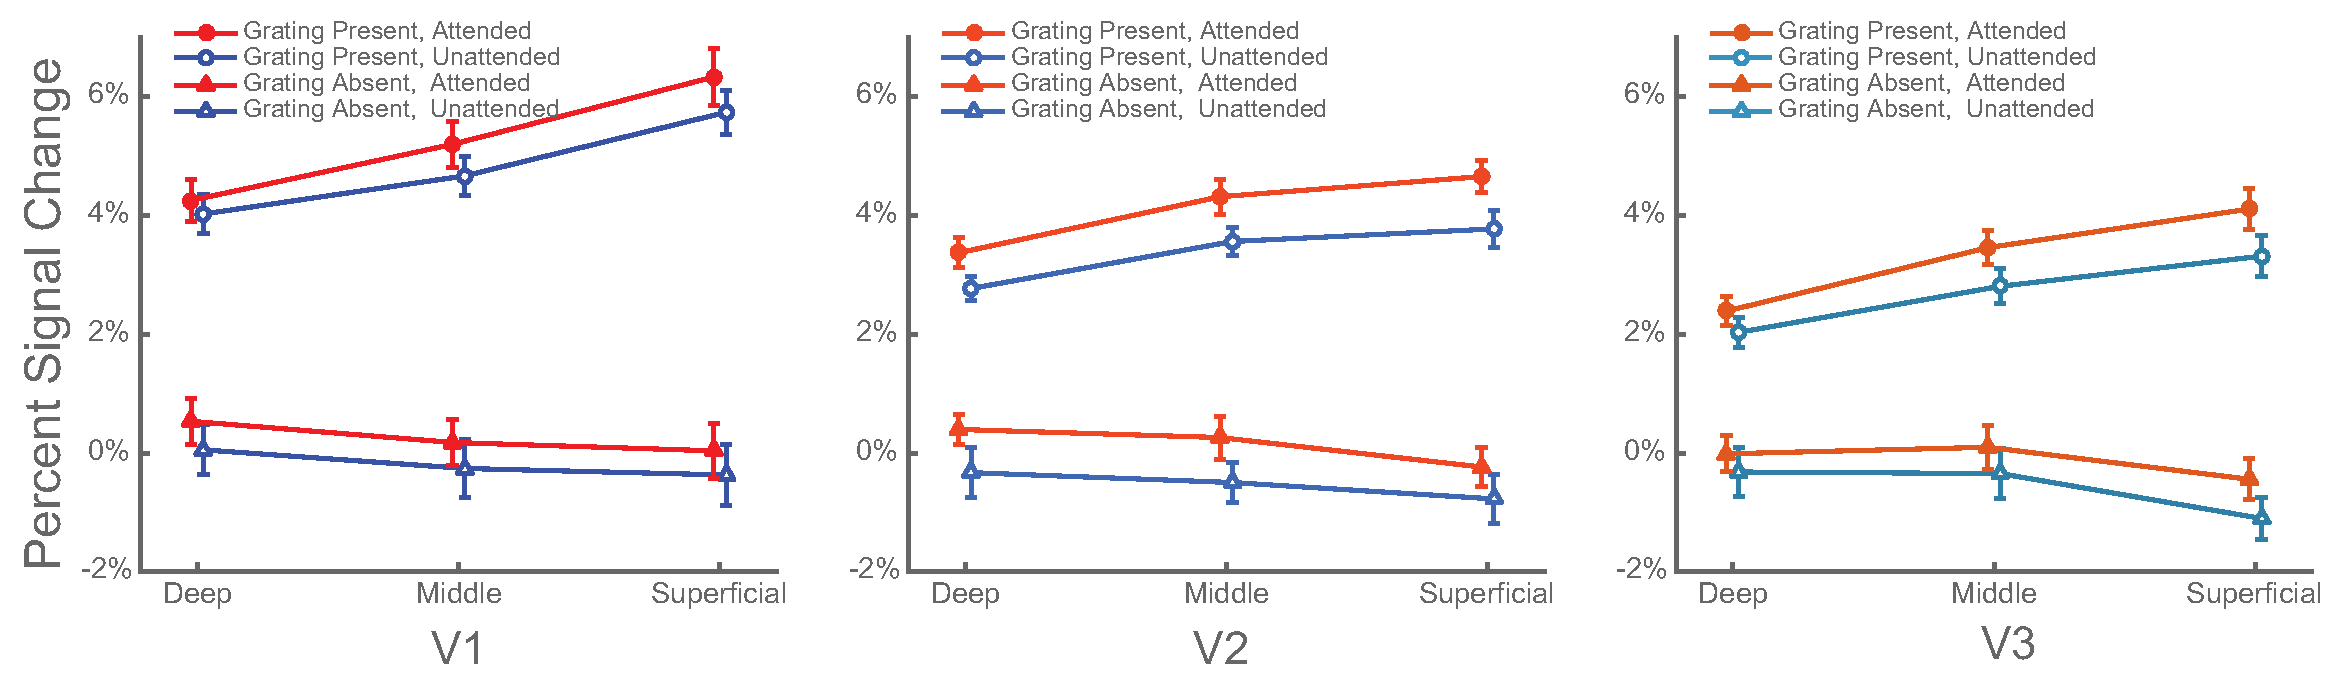
\includegraphics[width=1.0\textwidth, clip=true]{./Chapters/04_Attention/Images/SM_LayerResults_300vertices}
\caption{Control analysis of an ROI with the 300 highest activated vertices.}
\label{fig:layerresults300}
\end{figure}
\begin{figure}[!ht]
\centering
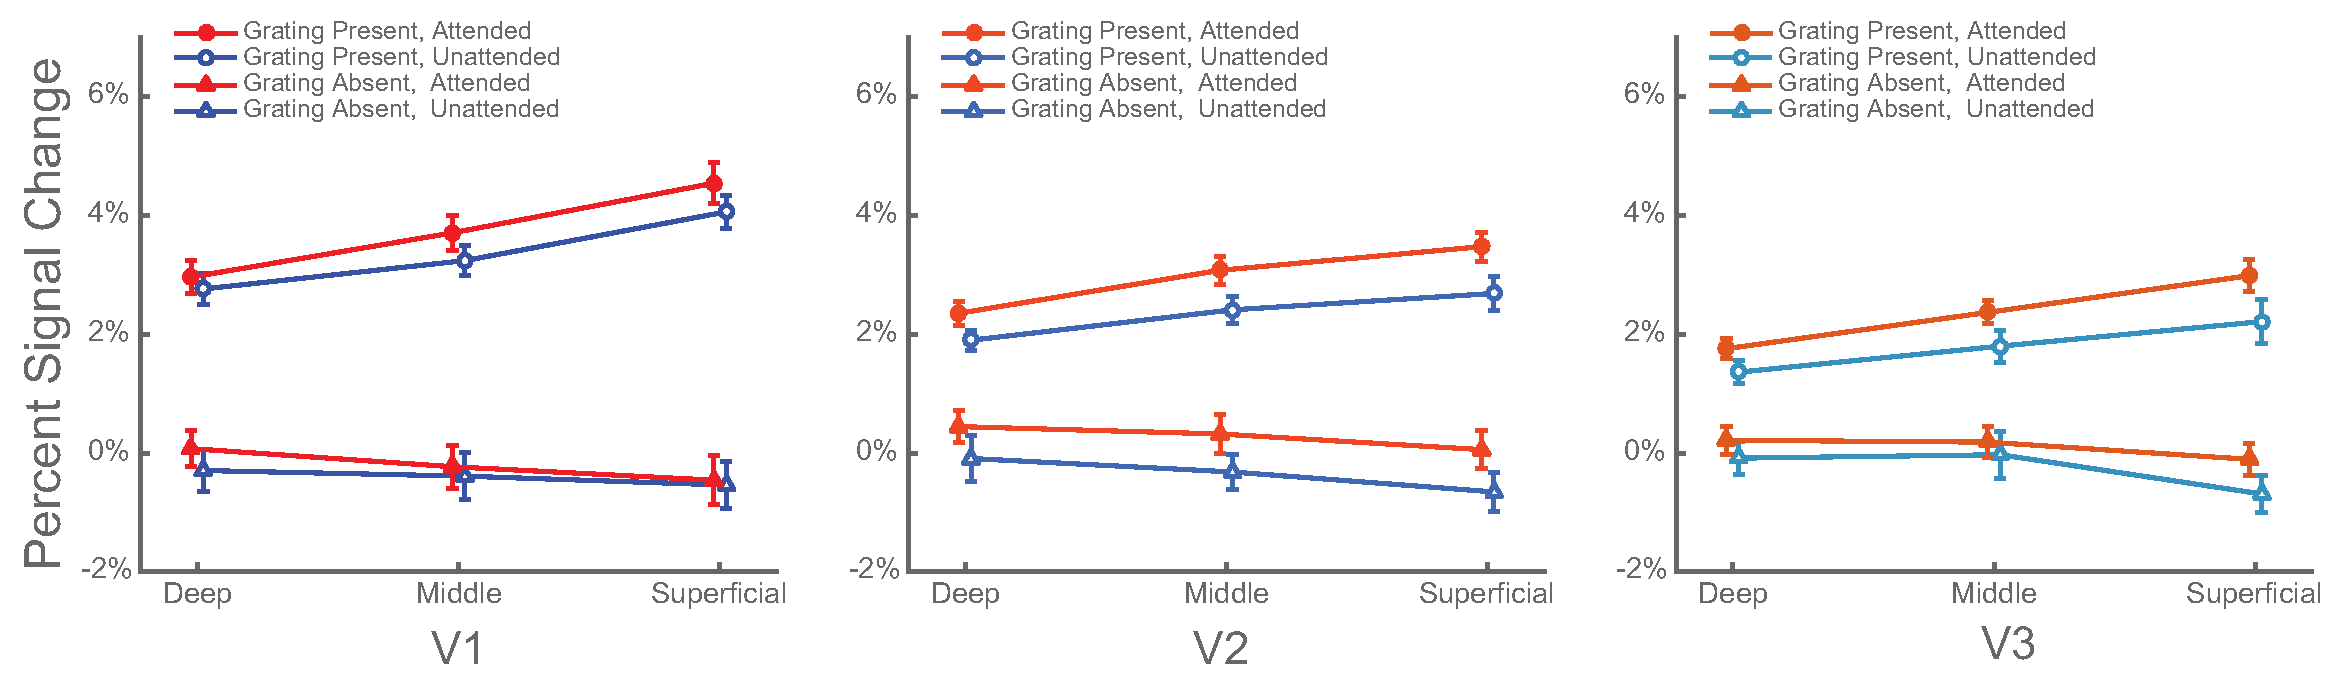
\includegraphics[width=1.0\textwidth, clip=true]{./Chapters/04_Attention/Images/SM_LayerResults_900vertices}
\caption{Control analysis of an ROI with the 900 highest activated vertices.}
\label{fig:layerresults900}
\end{figure}
\begin{figure}[!ht]
\centering
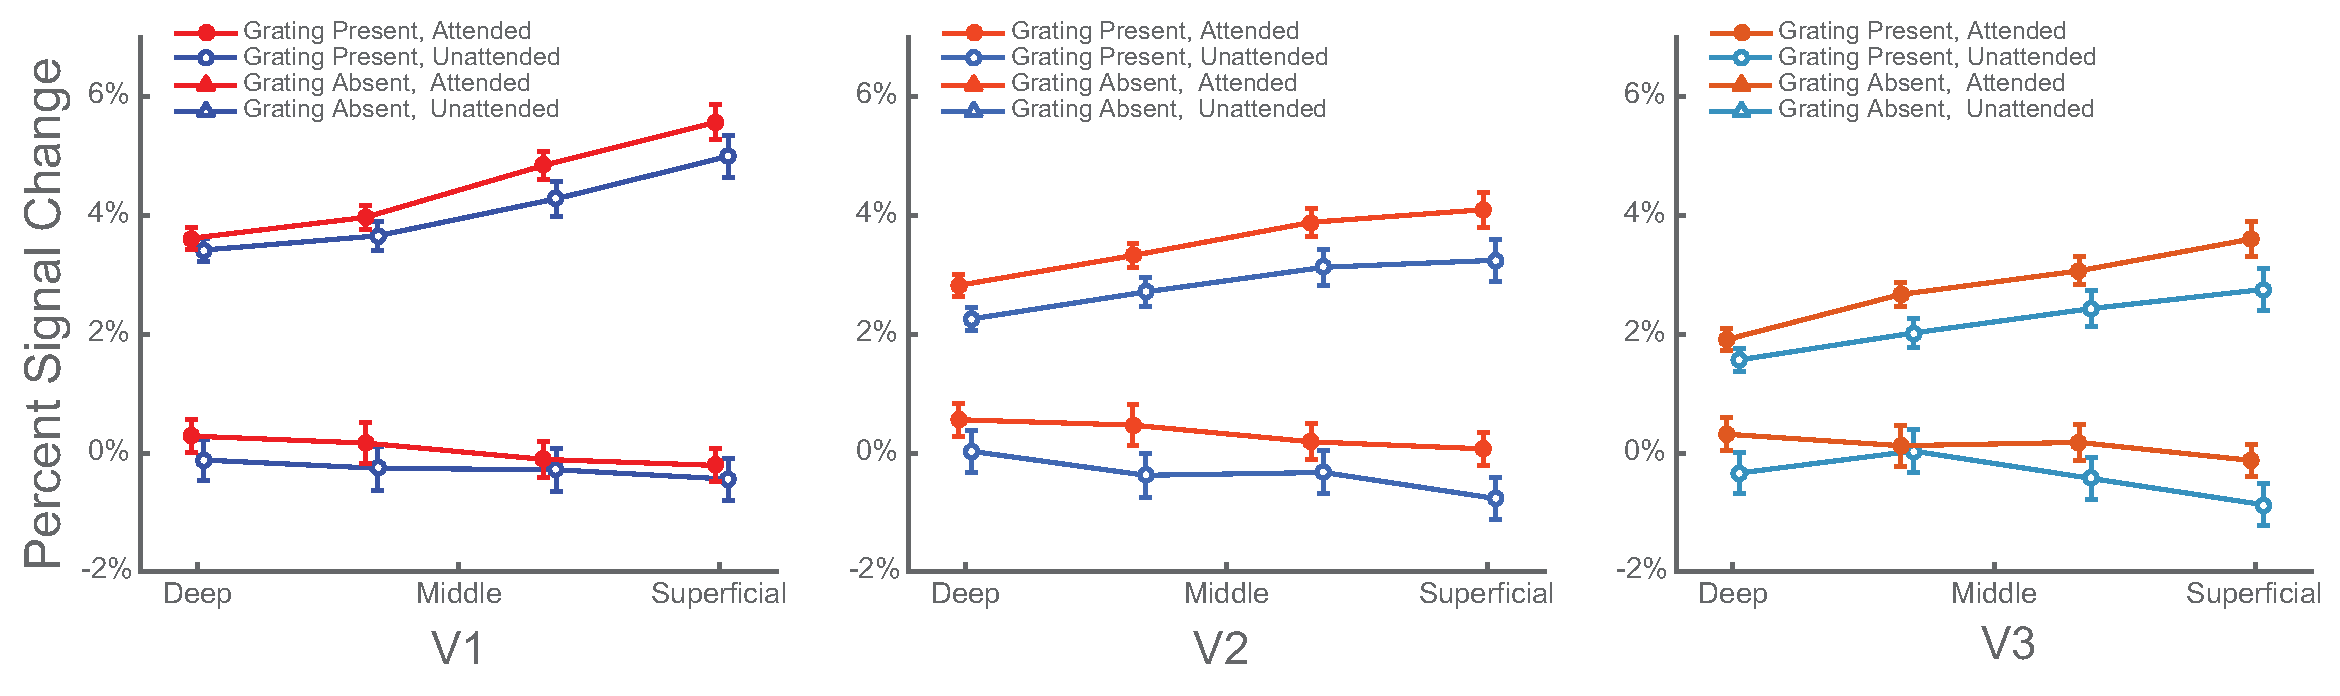
\includegraphics[width=1.0\textwidth, clip=true]{./Chapters/04_Attention/Images/SM_LayerResults_4Layers}
\caption{Control analysis of an ROI with the 600 highest activated vertices, within each of 4 layers.}
\label{fig:layerresults4layers}
\end{figure}
\begin{figure}[!ht]
\centering
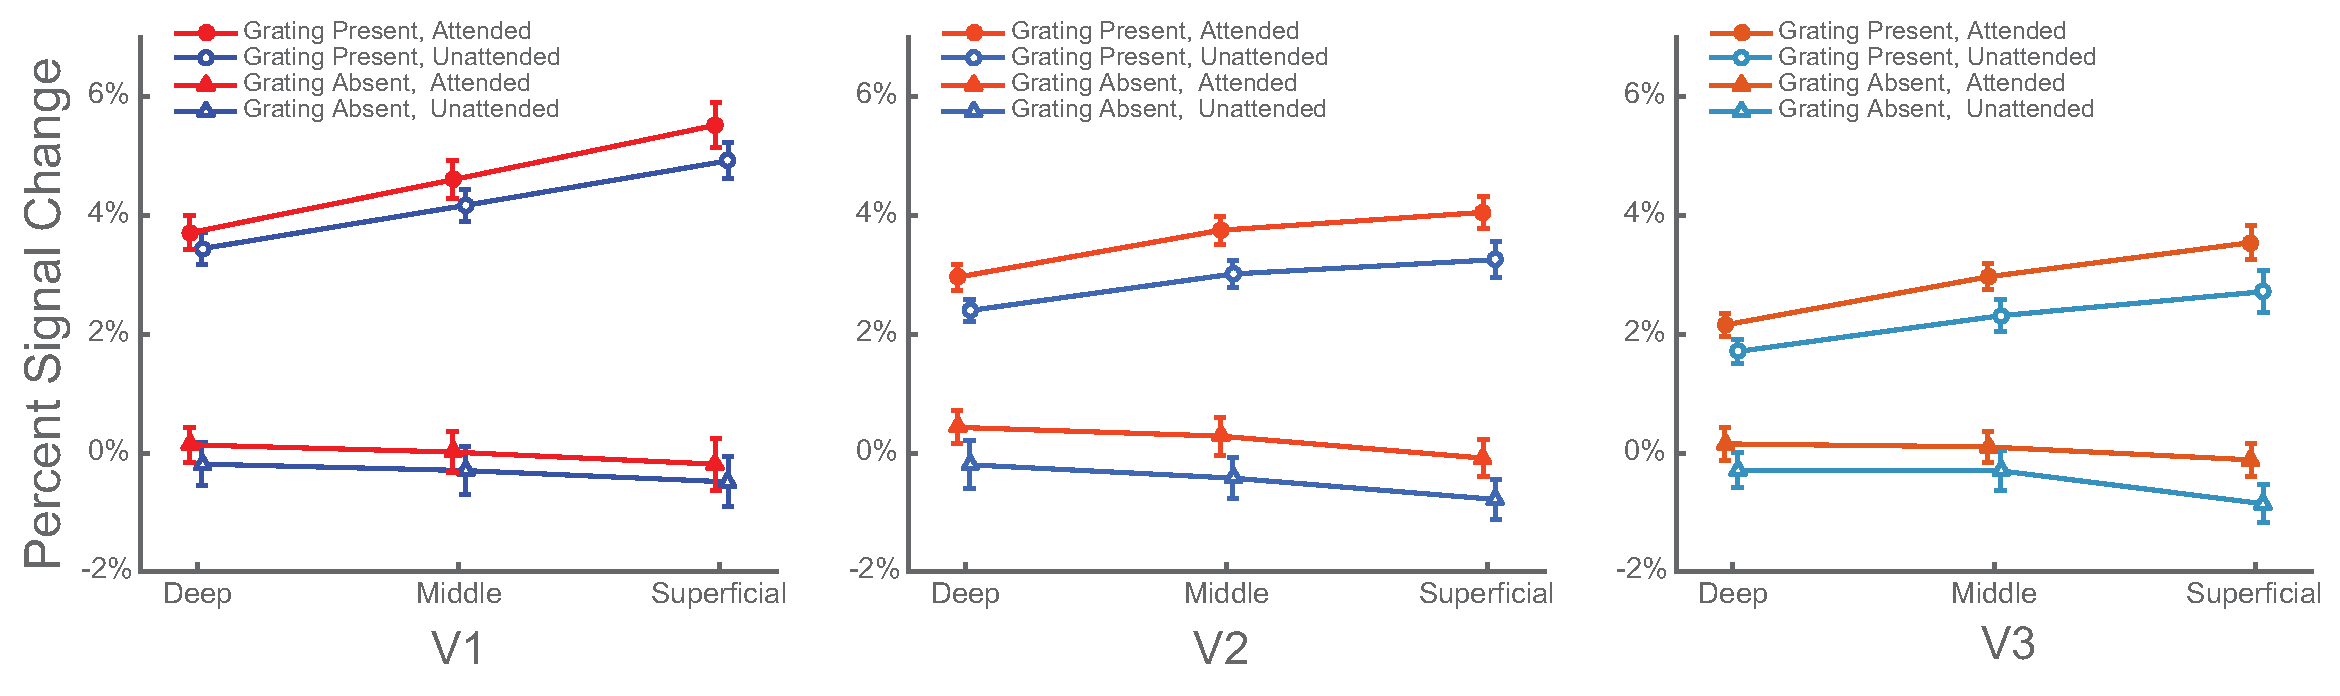
\includegraphics[width=1.0\textwidth, clip=true]{./Chapters/04_Attention/Images/SM_LayerResults_interpolation}
\caption{Control analysis of an ROI with the 600 vertices highest activated vertices, where the laminar signal was obtained by means of interpolation instead of a laminar spatial GLM.}
\label{fig:layerresultsinterp}
\end{figure}
\begin{figure}[!ht]
\centering
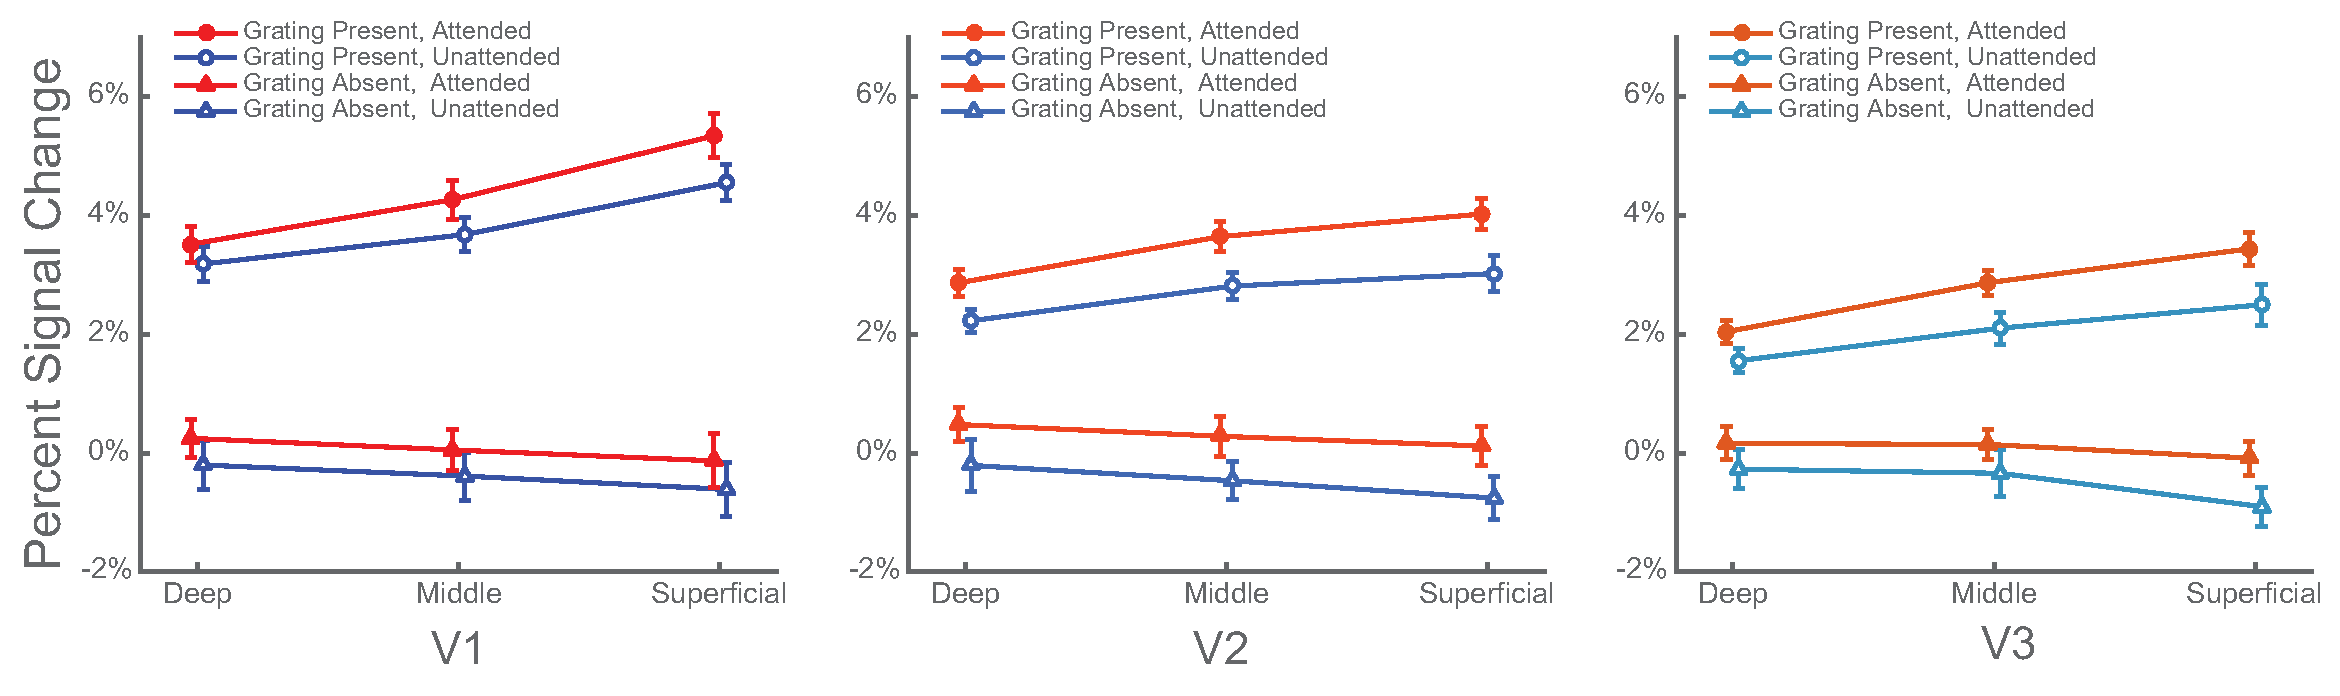
\includegraphics[width=1.0\textwidth, clip=true]{./Chapters/04_Attention/Images/SM_LayerResults_plusAttention}
\caption{Control analysis of an ROI with the 600 vertices highest activated vertices, where the signal from the anticipation window was added to the signal from the stimulus window.}
\label{fig:layerresultsplusattention}
\end{figure}
Figure S1-5. Layer-specific amplitude of the BOLD response in areas V1-V3. Figures S1 and S2 show stimulus and attention-based effects across layers after selecting, respectively, the 300 and 900 most activated vertices (cf. Fig.~\ref{fig:layerresults} in the main text). Figure S3 shows results after defining four cortical layers, rather than three, and Figure S4 depicts results obtained from interpolation instead of a laminar spatial GLM. Error bars indicate $\pm$1 SEM. For figure S5, the signal from the anticipation window was added to the signal from the stimulus window. In all Figures, presenting a stimulus (circles) resulted in a reliable increase in BOLD response from deep to superficial layers. The BOLD response was significantly enhanced for attended locations (red) compared to unattended location (blue) across layers, both when a stimulus was presented and in the absence of visual stimulation. There were only two instances where significance changed compared to the layer analyses that are presented in the main text. The Attention by Layer interaction was not significant in the main analysis (p = 0.114), but was significant in the control analysis when interpolation was used (p = 1.50$\cdot10^{-4}$) and when the signal from the anticipation window was added (p = 0.019). While the Stimulus by Layer by Area interaction was significant in the main analysis (p = 0.015), this interaction failed to reach significance after selecting the 900 most activated vertices (p = 0.12), or when repeating the analysis using four (rather than three) layers (p = 0.056). All other reported results are qualitatively similar to the findings in the main text.
\label{SM5}
\begin{figure}[!ht]
\centering
\includegraphics[width=0.6\textwidth, clip=true]{./Chapters/04_Attention/Images/ExampleBrain}
\caption{Example of Regions of interest on the inflated cortical surface for a representative subject. The label contours from top to bottom show dorsal V3, V2, and V1 and ventral V1, V2, and V3, in both hemispheres. The 600 most activated vertices (highlighted) per region where selected for the main analysis, the 300 and 900 vertices for control analyses in order to show that the effects are independent of size of region of interest.}
\label{fig:roifigures}
\end{figure}
%Random Subject19


%300 vertices:
%The T-values in the region of interest ($\mu \pm \sigma$) were for V1 $T=3.414 \pm 0.950$, for V2 $T=2.728 \pm 0.726$ and for V3 $T=2.562 \pm 0.779$.


%900 vertices:
%The T-values in the region of interest ($\mu \pm \sigma$) were for V1 $T=2.637 \pm 0.828$, for V2 $2.002 \pm 0.715$ and for V3 $1.773 \pm 0.716$.



%A visualisation of the workflow is shown in Fig.~\ref{fig:workflow}.
%\input{./Chapters/04_Attention/Chapters/Figures/FigureWorkflow}






\chapter{Porcupine: a visual pipeline tool for neuroimaging analysis}
\chaptermark{Porcupine}
\label{ch:porcupine}

\textcolor{gray}{{Tim van Mourik$^{1}$}, Lukas Snoek$^{2}$, Tomas Knapen$^{3,4}$, David G Norris$^{1,2}$\\
$^{1}$Radboud University Nijmegen, Donders Institute for Brain, Cognition and Behaviour, Nijmegen, The Netherlands \\
$^{2}$University of Amsterdam, Department of Brain \& Cognition, Amsterdam, The Netherlands\\
$^{3}$Cognitive Psychology \& Institute for Brain \& Behavior, Amsterdam, the Netherlands\\
$^{4}$Spinoza Centre for Neuroimaging, Amsterdam, the Netherlands \\
$^{5}$Erwin L. Hahn Institute for Magnetic Resonance Imaging, University Duisburg-Essen, Essen, Germany}\\

%----------------------------------------------------------------------------------------
%	ABSTRACT
%----------------------------------------------------------------------------------------
\linespread{1.5}
\newpage
\section*{Abstract}

The field of neuroimaging is rapidly adopting a more reproducible approach to data acquisition and analysis. Data structures and formats are being standardised and data analyses are getting more automated. However, as data analysis becomes more complicated, researchers often have to write longer analysis scripts, spanning different tools across multiple programming languages. This makes it more difficult to share or recreate code, reducing the reproducibility of the analysis. 
We present a tool, Porcupine, that \change{allows the construction of analyses in a graphical user interface, and also automatically produces analysis code.}{constructs one's analysis visually and automatically produces analysis code.} The graphical representation improves understanding of the performed analysis, while retaining the flexibility of modifying the produced code manually to custom needs. Not only does Porcupine produce the analysis code, it also creates a shareable environment for running the code in the form of a Docker image. Together, this forms a reproducible way of constructing, visualising and sharing one's analysis. Currently, Porcupine links to Nipype functionalities, which in turn accesses most standard neuroimaging analysis tools. \change{With Porcupine, we bridge the gap between a conceptual and an implementational level of analysis and thus create reproducible and shareable science. We give the researcher a better oversight of their processing pipeline, both while developing and communicating their work. This will reduce the threshold at which less expert users can generate reusable pipelines.}{Our goal is to release researchers from the constraints of specific implementation details, thereby freeing them to think about novel and creative ways to solve a given problem. Porcupine improves the overview researchers have of their processing pipelines, and facilitates both the development and communication of their work. This will reduce the threshold at which less expert users can generate reusable pipelines. With Porcupine, we bridge the gap between a conceptual and an implementational level of analysis and make it easier for researchers to create reproducible and shareable science.} 
We provide a wide range of examples and documentation, as well as installer files for all platforms on our website: \url{https://timvanmourik.github.io/Porcupine}. Porcupine is free, open source, and released under the GNU General Public License v3.0.
\newpage
%----------------------------------------------------------------------------------------
\section{Introduction}
%Positive intro to set the stage)
The field of neuroimaging is rapidly adopting a more reproducible approach to data acquisition and analysis. Especially in recent years, a strong movement for conducting better documented and more reproducible science can be observed. Advances have been made in terms of openly sharing data (e.g. OpenFmri, \cite{Poldrack2013}), standardizing data formats (BIDS format \cite{Gorgolewski2016}), and facilitating more automated pipelines \cite{Fischl2004,Gorgolewski2011,Jenkinson2012}. These initiatives facilitate increasing global scientific communication and collaboration, that is paramount in the age of big data.

%Problem: software limitations
As a result of the increasing complexity of analyses\remove{, however,} and the wide variety of different tools, researchers often have to write custom scripts for combining different software packages, often in different programming languages. As an extra obstacle, many tools have external dependencies, intricate installation procedures, or different file formats for the same type of data. Furthermore, the sharing initiatives usually have a stronger focus on sharing \emph{data} (Human Connectome Project \cite{Elam2015}, NeuroVault \cite{Gorgolewski2015}) instead of \emph{code}, such that analysis scripts still have to be recreated based on the method section of a paper. All these factors negatively affect the reproducibility, documentation, and in the worst case correctness of the analysis \cite{Nosek2015}.
%and may be seen as a waste of money by the greater public, as most research is funded by the tax payer. 

%Problem: people limitations
A considerable mastery of coding is required for analysing fMRI data. The conceptual side of understanding all preprocessing steps is not trivial, but converting this into a working pipeline can be an arduous journey. The necessary programming skills are not usually the prime focus of a brain researcher's skills or interests, but they are a necessity for completing one's analysis. Consequently, scripting a pipeline that covers all high-level and low-level aspects is daunting and error prone. As a result, there is a considerable risk \change{one will revert to}{of} `hacking' an analysis pipeline together, sacrificing a reproducible approach. So as a researcher, how do you start an analysis? It is easiest to start with visualising the steps of your analysis pipeline.  

%Current solutions and shortcomings
In an increasingly complicated analysis environment there is a strong need for tools that give a better oversight of these complex analyses, while retaining the flexibility of combining different tools. A notable effort to integrate different tools is Nipype \cite{Gorgolewski2011}, that has a Python interface to existing tools from all major MRI analysis packages. However, this still requires non-trivial Python scripting. Furthermore, Nipype is only able to visualise a workflow after it has been manually scripted \cite{Ellson2002}.

%Our solution
Here we detail our solution to these problems, an open-source software program we call Porcupine: 'PORcupine Creates Ur PipelINE\remove{- the worst recursive acronym with bad capitalisation and annoying use of slang'}. Porcupine allows the creation of neuroimaging pipelines by means of a graphical user interface (GUI). After graphical pipeline definition, Porcupine in turn creates the code that programmatically defines the pipeline. Additionally and without any additional overhead, we supply a Dockerfile (\url{https://www.docker.com}) that automatically builds the run environment for the pipeline. This not only facilitates sharing the pipeline, but also ensures its reproducibility \cite{Boettiger2015}. We provide an extensive list of examples and documentation on our \href{https://timvanmourik.github.io/Porcupine/examples}{website}, as well as the possibility to upload one's custom pipeline to create a community driven library of analyses.

%Details about solution
By implementing an intermediate visual step in the generation of preprocessing workflows, Porcupine allows the user to focus on the logical flow of the preprocessing pipeline in a graphical representation without the need for coding at this conceptual stage of development. Because the GUI produces \change{working}{functional} analysis code, the user can\remove{then} immediately inspect, save, and run the generated code. Thus, Porcupine provides a stepping stone that eases the transition from concept to implementation. Because the entire pipeline and its parameters are defined \emph{in abstracto} before it is run, systems such as Nipype allow for elaborate checks and optimisations of the pipeline's execution. Furthermore, such systems can straightforwardly incorporate full logging of all analysis steps, creating a paper trail of the pipeline's execution. This combination of a reproducible environment in which a predefined pipeline is run by means of a system that provides precise bookkeeping paves the way to new standard that will ensure steady and reproducible progress in the field of cognitive neuroimaging \cite{Gorgolewski2016a}. 

%Concluding remarks
In our practical experience, the use of Porcupine allows one to very quickly prototype preprocessing pipelines. Novice users can create a pipeline \emph{de novo} and quickly focus on the code for this pipeline, greatly speeding up the learning process and thereby facilitating the use of reproducible pipelines. We envisage Porcupine to play a role in both the education of novice neuroimaging students and the rapid prototyping of pipelines by expert users. Here, we first outline several Porcupine use-case scenarios of increasing complexity, after which we detail the architecture of Porcupine.



\section{Results}
\subsection{What is Porcupine?}
%the general idea 
Porcupine is a graphical workflow editor that automatically produces analysis code from a graphically composed pipeline. By dropping 'nodes' (representing analysis steps) into the workflow editor and by connecting their data inputs and outputs, a pipeline is constructed. Analysis code is then automatically generated from the graphical representation of the pipeline. The code can readily be saved to a script (e.g. a Python, MATLAB, or Docker file) in order to perform the desired analysis. Additionally, the pipeline can be shared or inspected in visual form (PDF/SVG), or saved to a Porcupine specific (.pork) file to continue working on the pipeline at another time.

%the different panels idea
Apart from the visual representation of the pipeline, we provide more functionality to orderly structure one's analysis, as outlined in Fig.~\ref{fig:porcupine-editor}. All functions (the nodes in the graph) that are included in the pipeline are also listed in a separate panel, listing their input parameters, output data, as well as a link to the online documentation of the function. We also provide the option to iterate over any input variable in order to facilitate parallelisation over subjects, sessions, or other variables. All parameters may also be edited in a separate parameter panel of the user interface. This functions as a central storage for important parameters, for example the ones that should be reported in a methods section. Porcupine combines the graphical overview and the parameters to automatically create the analysis code shown in the code window. 
\begin{figure}[!ht]
	\centering
	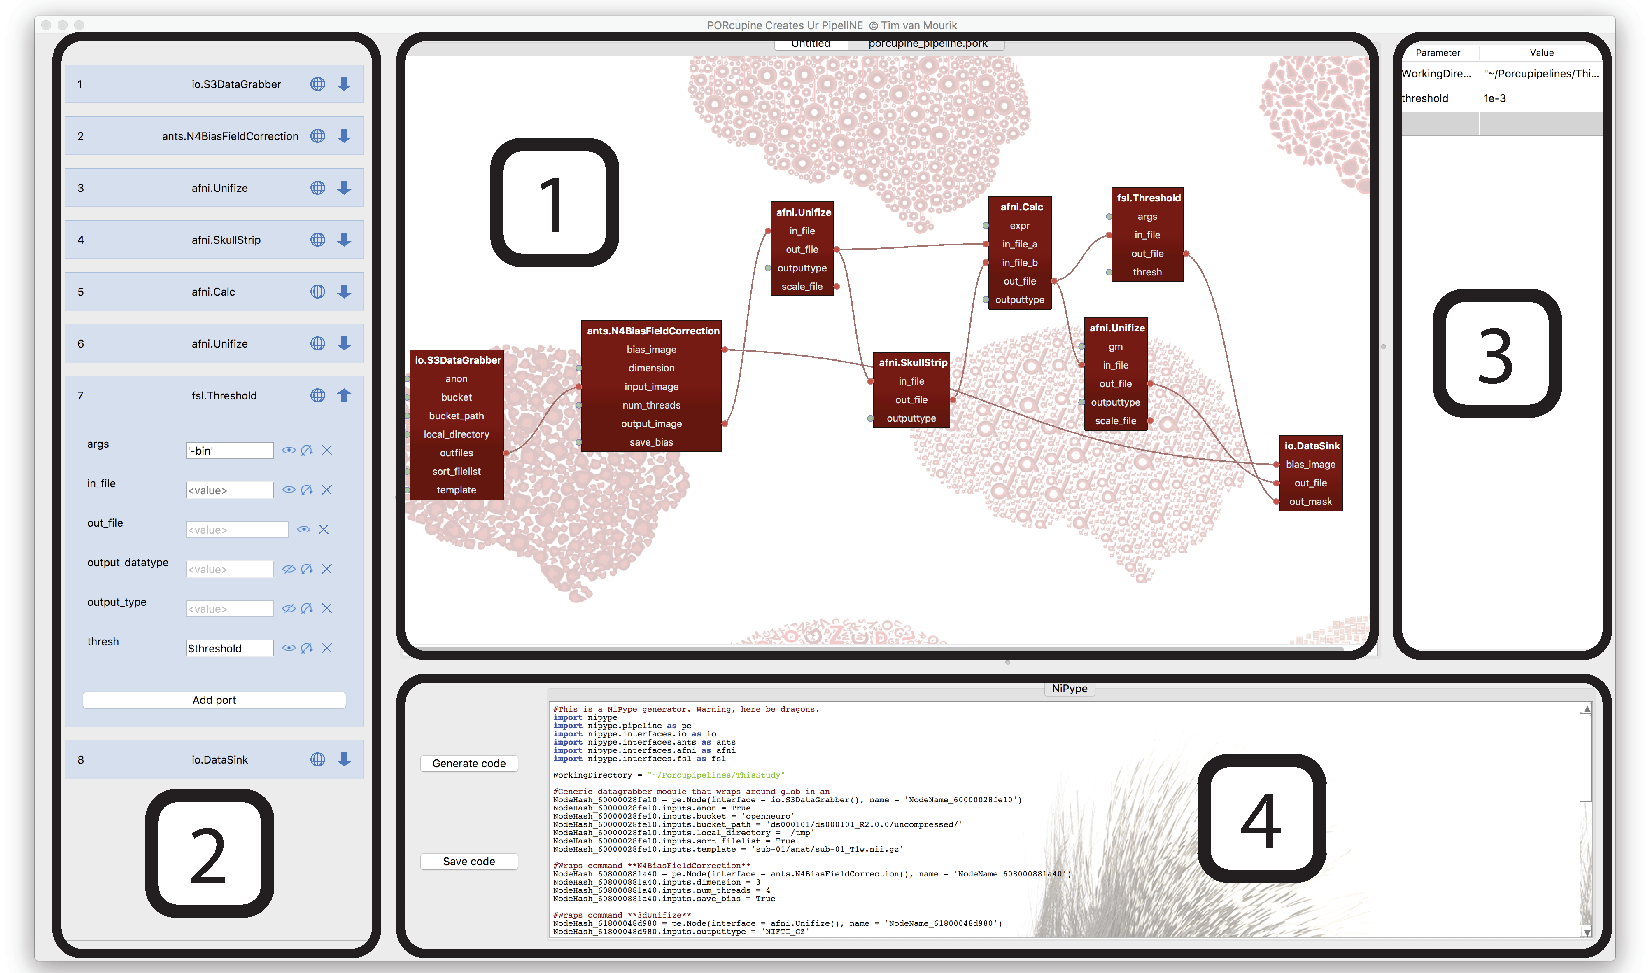
\includegraphics[width=0.9\textwidth, clip=true]{./Chapters/05_Porcupine/./Images/gui_showcase.pdf}
	\caption{A screenshot of a Porcupine workflow. The editor is divided into four panels, each of them targeted at facilitating a more understandable and reproducible analysis. The \emph{workflow editor} (1) provides a visual overview of one's analysis. The functions are all listed in the \emph{node editor} (2), where the parameters for all functions can be orderly stored. This may include links to important parameters that are listed in the \emph{parameter editor} (3), such that an overview of the main analysis settings can be easily viewed and modified. Readily executable analysis code is generated in the \emph{code window} (4)}
	\label{fig:porcupine-editor}
\end{figure}

%scope of this paper
We here focus on code generation that strictly adheres to the Nipype API \cite{Gorgolewski2011}, a Python-based MRI analysis and pipelining package. Nipype is used for its strong focus on uniformity in accessing functions, its link to most major MRI analysis tools, and its emphasis on reproducible science. Porcupine's architecture, however, is in principle agnostic with respect to the specific implementation of the underlying pipelining software. Any package with a consistent interface in the field of e.g. neuroimaging, bioengineering, or astronomy could benefit from using Porcupine's architecture.

%show by example
We first show that we can easily generate a standard fMRI analysis pipeline. After visually dragging and dropping modules, code is automatically created that is usually scripted manually instead. We then show how we facilitate loading data from an online repository, generate a readily executable fMRI pipeline, but also generate a shareable and reproducible analysis environment (using Docker), all with minimal additional effort. This allows for easily scalable analyses that \change{could}{can} be performed locally, but also on computational clusters or with cloud computing, without manual installation of different software packages. 

\subsection{Usage example}
We here show a simple example that constructs a pipeline for a single operation. In three steps, data is loaded, (minimally) processed, and the output is written to disk, as shown in Fig.~\ref{fig:porcupine-simple}. We here show an example that links to an OpenNeuro fMRI data set, but we could load any online data set that is set up according to the BIDS format \cite{Gorgolewski2016}. OpenNeuro's data sets are stored as Amazon repositories (`S3 buckets') and can be loaded by dragging the appropriate module into the workflow editor and typing the name of the bucket into the node editor. Its output can subsequently be connected to a Nipype function node, for example FSL's Brain Extraction Tool. All parameters of the function are listed and can be set in two different ways: either by dragging a link from a previous node's output port to an input port in the next node, or by typing in the parameter in the node editor. Subsequently, output can be written to disk by connecting the desired output to a Nipype DataSink node that collects and stores the data. By pressing the `Generate code` button, the code for this pipeline is automatically generated and can immediately be saved and executed in a Python shell.
\begin{figure}[!ht]
	\centering
	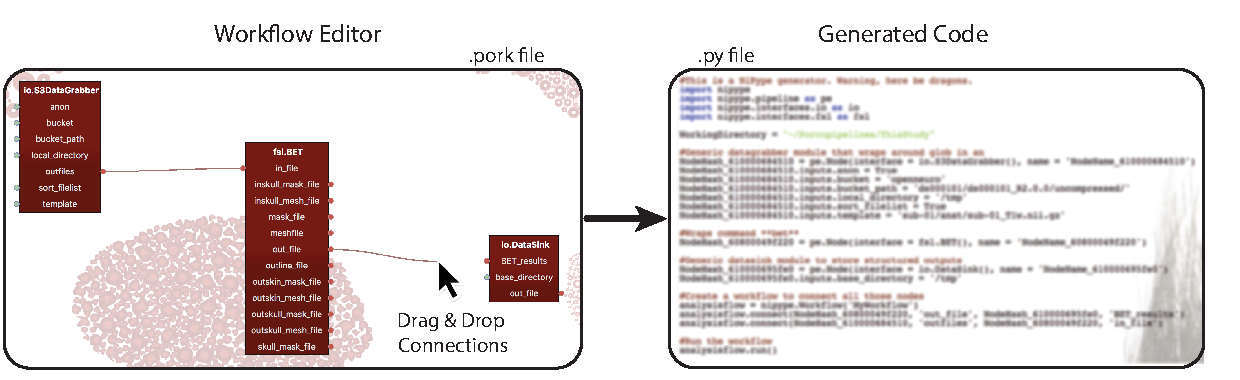
\includegraphics[width=0.9\textwidth, clip=true]{./Chapters/05_Porcupine/./Images/pork_py.pdf}
	\caption{An example of simple workflow. In three steps, this pipeline loads data, processes it, and writes it to disk. This is achieved by connecting the input and output fields from subsequent nodes in the pipeline. The constructed workflow is then transformed in readily executable (Nipype) analysis code.}
	\label{fig:porcupine-simple}
\end{figure}


\subsection{Pipeline sharing}
From a simple example that reads and writes the data, a more complicated pipeline is readily set up. More functionality, i.e. nodes, can be dragged in and connected to quickly build a custom pipeline. As it is commonplace to repeat a single analysis or function for several subjects, sessions, or other variables, every field can be flagged as an `iterator' field. This facilitates looping over variables. Once the pipeline is set up and the code is generated, Nipype offers functionality to construct a visual pipeline graph from custom python code. In Porcupine's proposed use-case, this end point of a standard Nipype pipeline represents the starting point, as shown in Fig.~\ref{fig:porcupine-advanced}. This allows the user to focus on the desired pipeline graph first, and then progress to the manual editing of the generated code.
\begin{figure}[!ht]
	\centering
	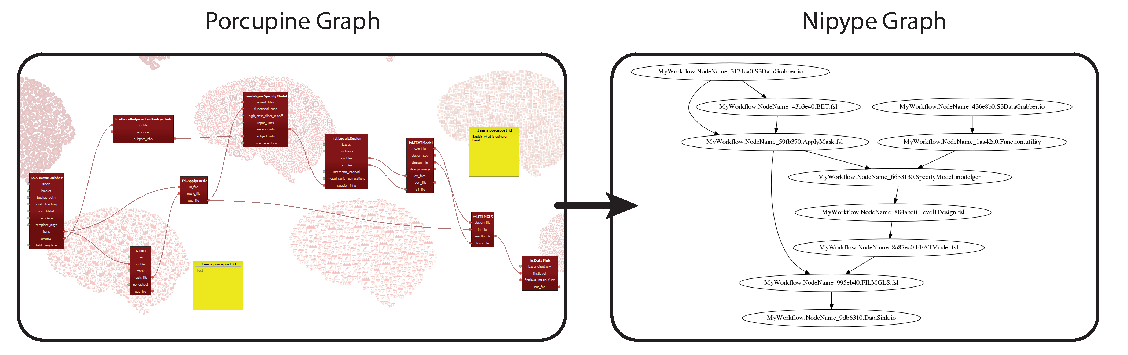
\includegraphics[width=0.9\textwidth, clip=true]{./Chapters/05_Porcupine/./Images/pork_graph.pdf}
	\caption{An example of a more complicated and realistic fMRI preprocessing pipeline. Once the code is generated, this can in turn be transformed into a Nipype graph visualisation. Whereas this is usually the end point for a pipeline in Nipype, we here propose to use a visualisation as a starting point of one's analysis.}
	\label{fig:porcupine-advanced}
\end{figure}

Not only does Porcupine provide a way of setting up a preprocessing  or analysis pipeline, we also provide a means for executing these pipelines in a reproducible environment. In addition to the Python analysis file that is generated, we create a scaffold for a Docker file. Docker (\url{https://www.docker.com}) is an open platform to easily build, run and share applications. The generated Docker file describes a minimal operating system that is required to run the analysis, based on the dependencies of the modules used in the workflow editor. With this Docker file, an image of the full analysis can be built, shared and executed. This provides a simple platform to reproduce results of one's analysis, on the same data set, or on another with only a single change in the data source module. Alternatively, one can use it as a template environment for a new follow-up analysis. As with all generated code, the Docker code is fully customisable to a researcher's need, but our suggested scaffold requires only a single manual edit to be built as a Docker image (see~\nameref{app:docker}). The Docker command will execute the pipeline: load the data from an online repository, process the data, and store only the output data to a local directory. The Docker image includes both the pipeline code and the run environment, and can be shared alongside a paper via DockerHub. The above examples (and many more) as well as extensive documentation and tutorials can be found \href{https://timvanmourik.github.io/Porcupine}{here}.

\subsection{Limitations}
Some features in Nipype have not been implemented. Notably, the JoinNode functionality is not yet accessible from the Porcupine user interface, in which the results from an upstream iterator are aggregated to a single output. Furthermore, custom extensions of Nipype functions are not automatically supported, but we do provide a script to add one's own custom module to Porcupine that would make this functionality accessible. A GUI for this is still an intended point of improvement. In general, feature requests are maintained as \add{\emph{issues} and} \emph{projects} in the \href{https://github.com/TimVanMourik/Porcupine/projects}{GitHub repository}. We encourage people to contribute new ideas or implementations for functionality in terms of modules, new toolboxes, and, most importantly, custom pipelines that can be added to the repository. Details \change{for contributing}{on how to contribute} can be found on the website.

While Porcupine in principle supports all workflow operations, a specific pipeline may well require modules that are not provided within Nipype. It is advised that the user either packages custom code for this into a new module, or manually adds it to the produced code. \change[Reviewer 2]{Porcupine itself functions only as the front-end to the Nipype back-end, but}{We furthermore stress that Porcupine is intended to function as a front-end encapsulation of NiPype, and does not implement the parsing of python files that contain pre-defined nipype pipelines. It also} does not perform type-matching on the input and output of a connection, nor does it perform syntax checking of the manually edited parameters.
\section{Design and Implementation}
Porcupine's graphical user interface was written first with a general visual programming application in mind. The initial interface to Nipype was developed at a three-day coding sprint at BrainHack 2017, Amsterdam. This kickstarted Porcupine in its current form. The source code, as well as the installer files for Windows, Mac, and Linux, are publicly available as a \href{https://github.com/TimVanMourik/Porcupine}{GitHub repository}. Porcupine is free, open source, and released under the GNU General Public License v3.0. \add[Reviewer 1]{It has static digital object identifier (DOI)} \url{doi.org/10.5281/zenodo.1146653}.

Visual programming is a generic way of programming to create a data flow or to perform an ordered task with a modular structure \cite{Myers1986}. Customarily, it allows the user to construct a Directed Acyclic Graph (DAG) \cite{Thulasiraman1992} of conceptualised operations that are subsequently interpreted or compiled as an application \cite{Myers1990}. This format is particularly useful for workflows that fit modular structures, such as most neuroimaging data analyses \cite{Rex2003}. 

\subsection{Architecture}
Not only do we intend researchers to make their analyses (re-)usable and robust, our software also adheres to all 20 simple rules that were laid out to this end \cite{List2017,Taschuk2017}. The updates as well as the releases of the source code are realised by means of a GitHub repository. Installer files are provided for all platforms and do not require administrator privilege. Users are aided in getting started quickly by extensive documentation and an example gallery.

Easy cross-platform installation or compilation was achieved by programming Porcupine as a stand-alone application in Qt Creator (\url{https://www.qt.io}) for C++. Internal file formats were standardised to JSON dictionaries, a format native to Python, Qt, and web applications. This provides a simple means to add new modules to Porcupine, without the need to write additional code. Every dictionary specifies a software package (e.g. `Nipype', `Docker', etc.) that is interpreted by Porcupine and creates code that is native to the package. A package-specific interpreter needs to be written just once, after which new modules that are included in the dictionary will be automatically available in Porcupine.

%the dictionaries
Each JSON dictionary describes a list of functions (internally referred to as 'nodes'). Each function has a name and (optionally) a category, a web url to its documentation, and a block of code. A code block specifies the software package for which the node is meant, the associated piece of code for that function and optionally an additional comment. Furthermore, a node contains any number of data/parameter ports, each of which can be input, output, or both. Optionally, additional flags can be set for ports to be visible in the editor, whether its value is editable, or whether the variable needs to be iterated over. Thus, JSON files for custom nodes can easily be created and added as a dictionary to the graphical interface. We also provide a Python script that converts a custom Python function(s) to a Nipype node dictionary.

\subsection{Extending Porcupine with new toolboxes}
Currently, Porcupine features Nipype and Docker support, but this could easily be extended to other software packages. This requires no major changes to the Porcupine source code, merely the inclusion of a single C++ class that describes the relationship between the nodes, links, and the output code. Specifically, the `CodeGenerator` class must be inherited and has access to the full workflow: the list of nodes, their parameters, and their connections. As long as all functions within an analysis toolbox can be accessed with a consistent interface, they can be represented as modules within Porcupine. Apart from Nipype, support for a laminar specific fMRI analysis toolbox in MATLAB is provided. The developers of the Fastr framework programmed initial support for their code base \cite{Achterberg2016}. Unfortunately, only few neuroimaging packages abide by this uniformity of their functions and hence many cannot be included into Porcupine.

\subsection{Relation to existing pipeline managers}
Porcupine aims to provide an extendable, transparent and flexible platform to build preprocessing and analysis pipelines. Other software packages have made similar attempts at providing visual aids to build or run pipelines. Within neuroimaging, the most notable ones are the JIST pipeline \cite{Lucas2010}, extended with CBS Tools \cite{Bazin2014} and the LONI pipeline \cite{Rex2003}. Porcupine distinguishes itself from these by not creating a run environment, but instead creating the analysis code for the researcher. This retains the possibility of immediately running the code through a Python interpreter, but also creates more flexibility, as researchers can modify and adjust the script according to their needs.\remove[Reviewer 3]{Additionally, as the functions link to existing Nipype interfaces, error reporting is more transparent such that problems can more easily be resolved.} Lastly, our open-source framework is set up to be extendable with new modules within existing frameworks, as well as with completely new frameworks. This provides a future-proof set-up for current and future analysis tools in neuroimaging and perhaps other disciplines.

\section{Availability and Future Directions}
We have presented a new tool to visually construct an analysis pipeline. Subsequently, Porcupine automatically generates the analysis code, and provides a way of running and sharing such analyses. We see this as an important tool and a stepping stone on the path to doing more reproducible and open science. Additionally, this gives researchers a better oversight of their analysis pipeline, allowing for greater ease of developing, understanding, and communicating complex analyses.

Porcupine provides two independent functionalities that dovetail to allow users to more easily take part in reproducible neuroimaging research. They are (1) a graphical user interface for the visual design of analysis pipelines and (2) a framework for the automated creation of docker images to execute and share the designed analysis. 

We anticipate that the ability to design processing pipelines visually instead of programmatically \change{cuts}{will cut} the novice user's learning phase by a considerable amount of time by facilitating understanding and development. The ease of use of a Graphical User Interface (GUI) implementation extends and complements Nipype's flexibility. Thus, it invites researchers to mix and match different tools, and adhere less stringently to the exclusive use of the tools of any given toolbox ecosystem. This flexibility enhances the possible sophistication of processing pipelines, and could for instance be helpful in cross-modal research or multi-site research. Additionally, it may nudge method developers to write new tools in a way that easily integrates with the Nipype and Porcupine structure.

The emphasis that Porcupine puts on visual development of analyses makes it easier to communicate a methods section visually rather than in writing. We foresee that researchers may prefer explicity sharing the created .pork files and the Nipype pipelines that are created from them, instead of solely relying on written descriptions of their methods. Yet another use case for Porcupine is the easy definition of proposed processing workflows for preregistered studies.

Importantly, Porcupine attempts to reduce the steepness of the learning curve that is inherent to the use of complex analysis, by providing a more structured and systematic approach to pipeline creation. It separates the skill of building a conceptual analysis pipeline from the skill of coding this in the appropriate programming language. This places Porcupine in a position to aid in the education of novice neuroimaging researchers, as it allows them to focus on the logic of their processing instead of the creation of the code for the processing - greatly improving and accelerating their understanding of the different steps involved in the preprocessing of neuroimaging data. At the same time, it allows more experienced researchers to spend more time on \change[Reviewer 2]{theconceptual}{the conceptual} side than on implementational side.

Having allowed for the visual design of a pipeline for the preprocessing or analysis of a neuroimaging dataset, the reproducible execution of this pipeline is another step that Porcupine facilitates. By flexibly creating a Docker image tailored to the different preprocessing steps defined visually in the GUI, Porcupine allows the user to share not only the definition of the pipeline but also its execution environment. This step removes the overhead of having to manually install the desired operating system with the matching distribution of MRI analysis software. This final step greatly facilitates the reproducibility of reported results, and is part of a general evolution of the field towards easily shareable and repeatable analyses. 

The generated Docker image can be made High Performance Computing aware \remove{with singularity} by means of dedicated tools such as \href{https://github.com/singularityware/docker2singularity}{docker2singularity}. Alternatively, with only trivial additions to the Dockerfile, it can be transformed into a BIDS app \cite{Gorgolewski2017}. A detailed explanation for doing this can be found on our \href{https://timvanmourik.github.io/Porcupine/documentation/advanced/make-a-bids-app}{website}. An automatic and direct way of creating \add{this} has not yet been implemented. Additionally, integrating support for standardised workflow file formats, such as the Common Workflow Language \cite{Amstutz2016} could further add to Porcupine's aim of reproducibility. Another point of improvement is a functionality to embed pipelines within pipelines. Currently, a complicated pipeline\remove[Reviewer 2]{s} does full justice to the term `spaghetti code', and the number of nodes and links may easily compromise the visual aid in understanding; the very purpose for which Porcupine was created. This may easily be solved by compartmentalising pipelines into logical units by providing an embedded structure.

We intend Porcupine to be a strong aid for doing better, more reproducible and shareable science. By bridging the gap between a conceptual and implementational level of the analysis, we give scientists a better oversight of their pipeline and aid them in developing and communicating their work. We provide extensive and intuitive documentation and a wide range of examples to give users a frictionless start to use Porcupine. We look forward to adding more functionality and\change{support for}{supporting} more toolboxes in the near future.

\section{Supporting information}
\paragraph*{S1 Docker files}
\label{app:docker}
Porcupine provides a Docker image that creates the necessary run time environment for a pipeline that is constructed in the workflow editor. As with all generated code, the Docker code is fully customisable to a researcher's need, but our suggested scaffold requires only a single manual edit to be built as a Docker image. A Docker script can only refer to online or on-disk resources, so the pipeline file needs to be saved manually and added to the Docker file:
\begin{lstlisting}
ADD /path/to/pipeline/script.py /somewhere/porcupipeline.py
CMD ["python", "/somewhere/porcupipeline.py"]
\end{lstlisting}
Once this line is added, the docker image can be built:
\begin{lstlisting}
$ docker build -t mydockerimage -f Dockerfile
\end{lstlisting}
The output from the executed pipeline can be written to a local directory on a researcher's computer (`/my/local/directory') by mounting it to the docker output directory (`/data') with the `-v' option and running the image as if it were a standalone application.
\begin{lstlisting}
$ docker run -v /my/local/directory:/data mydockerimage
\end{lstlisting}
This Docker command will execute the pipeline: load the data from an online repository, process the data, and store only the output data to a local directory. A fully worked out example with detailed explanation can be found \href{https://timvanmourik.github.io/Porcupine/documentation/basics/building-dockerfiles}{here}.
\section{Acknowledgements}
We would like to  thank the organisation of BrainHack Global and BrainHack Amsterdam, specifically Pierre-Louis Bazin, for organising the platform that kickstarted Porcupine in its current form. Tim van Mourik acknowledges support by Spinoza grant SPI 40-118.
\section{Author contributions}
TvM wrote the Porcupine C++ software. TvM, LS, and TK designed the interface to Nipype. LS and TvM built the website. LS wrote the examples and the majority of documentation. TvM, TK, LS, and DGN wrote the paper.


\chapter{Summary and Discussion}
\chaptermark{Discussion}
\label{ch:discussion}

For long the nature of the processing undertaken by the cortical layers has been recognised as a mystery that needs to be resolved to better understand the computations being performed by our brains \cite{Miller2001}. The most realistic method to date of studying this in living human subjects is with functional MRI, as it it very precise and non invasive. But many challenges in spatial and temporal resolution, resolution, interpretation, and all sorts of noise have to be overcome before this can be easily used to solve neuropsychological problems. The objective of this thesis was to pave the way for doing more routine laminar fMRI analysis. Indeed we made significant steps towards this end. 
We have developed several new methods that solve major problems in laminar analysis, we conducted a full layer specific analysis, and took explicit care to make everything along the way reproducible and reusable. %% <-- unpack

\section*{Chapter 2: Recursive Boundary Registration}
First, we addressed the problem of local distortions that are often present in Echo Planar Images (EPI). Due to inhomogeneities in the main magnetic field, spins in some areas rotate a bit faster or slower than others. Effectively, this causes small shifts of parts of the image with respect to the true position. Thus, even though the true locations of the layers are known, the distortions may easily be larger than the thickness of the layers. Without correcting this effect it is hopeless to get out any reliable layer signal. So that is what we set out to do in Chapter 2.

Geometry transformation from one volume to the other (coregistration) has been very succesful for linear transformations and is used routinely in fMRI analysis. Even on volumes with low resolution, low contrast, or few slices, it may work well \cite{Greve201}, but not for non-linear transformations. Such transformations require a high number of degrees of freedom because of the many parameters that need to be estimated. This leaves much more room for error and therefore usually only works on high contrast data sets. It is used routinely for transforming single subject anatomical space to a template space with the same contrast. However, existing techniques are not powerful enough to undistort low contrast EPI images. We therefore invented a new technique for this, Recursive Boundary Registration. By recursively applying linear transformations on diminishing spatial scales, we effectively compute a non linear registration. In order to guarantee smoothness over all transformations, it is combined with a control point lattice that regulates the transformations. Explicitly taking the geometry of the volume into account as a type of prior knowledge is a novel way to approach non linear registrations.

We tested RBR on two different types of data. First, in order to establish a gold standard, we distorted a FLASH image that is typically without distortion. Because we did this in a controlled manner, we could easily compare the performance of RBR to our ground truth and verify the quality of the registration. We thus proceeded to EPI data set of 11 subjects that had real distortions. As the true size of the distortions was unknown there cannot be an absolute quality metric for the registration. Instead, by adding different levels of noise we showed that there is a clear SNR dependance in the displacement that decreases towards the no-noise condition. Additionally, we provide an abundance of graphical evidence to illustrate the performance of RBR.

The power of the method lies in the fact that it makes explicit use of the gyrification of the brain and the specific geometry of an individual brain. It can therefore get away with little contrast and still produce an accurate registration while preserving the topology of the original. Because of the large number of parameters that needs to be estimated we built in a variety of robustness assurances. Despite the overall improved registration, it is still important to carefully inspect the quality of the registration to verify the required submillimetre accuracy. All in all, this proved to be a valuable tool for preparing Gradient Echo images for subsequent analyses and we use it in our experimental study in Chapter 4. It is now an integral part of the fMRI analysis toolbox for laminar fMRI, \url{https://github.com/TimVanMourik/OpenFmriAnalysis}.

An helpful realisation in developing this method was a more conceptual look on the problem. The problem of coregistration can be classified along two main axes: the type of image contrast can be different or the same, and the required transformation can be linear or non linear. The easiest scenario is to find a linear transformation for a volume with similar contrast. The problem becomes harder when the volume has a different contrast, as the mapping of intensity values from one volume to the next is unknown. If instead the contrast is the same but the required transformation is non linear, it is still solvable to a good approximation \cite{Collins1995}. However, when the contrast is different \emph{and} the registration should be non-linear the, the degrees of freedom of the problem increases drastically, and is not easily estimated anymore. Combine this with the low contrast-to-noise ratio of fMRI data and it is clear that this is a hopeless endeavour with standard volume-to-volume registration. The trick to solve this conundrum is to introduce more prior knowledge to the equation. In this case, we chose to use the geometric information of the cortex and its many gyri and sulci to more accurately estimate a non linear cross-modal registration. This does the trick on a single subject level, but by introducing prior knowledge, we restricted the use cases. Where the previous non-linear transforms could also compute subject-to-template registration, we lost this ability by strictly enforcing equal geometry across volumes. As a general notion, algorithms can become more powerful when they are more specialised. Usually this requires a specific type of prior knowledge in the data that is quantified and optimised.

\section*{Chapter 3: Spatial GLM for laminar fMRI}
Once the geometry of our cortical surfaces is properly aligned with our functional data, there is a next problem: how can the laminar signal be extracted from the MRI volume? There are several intuitive ways. A volume could simply be interpolated at the approximate location of the layers, or classify voxels to be part of it most likely layer. However, it is clear that this inherently smears out the laminar signal to some extent. In Chapter 3 we set out to quantify this signal leakage and to present a new method to reduces it and to more cleanly separate the laminar signal.

We started out with the notion that all voxels are a mixture of a variety of layers. If this mixture could be accurately modeled it could theoretically also be inverted and solved for the layer intensity values by means of the framework of the General Linear Model (GLM). To achieve this, we first set up a mathematical framework to accurately model the layer distribution and subsequently estimate the layer signal intensity. 

Our cortex model incorporates information about the precise location, curvature and thickness of the cortex to model the 



We previously mentioned that methods can become more powerful when they use types of prior knowledge inherent to the data. We here find that this is true, but might come at the cost of a la

The prior knowledge 


Due to the many factors that could play a role in the 
The combinatoric explosion of the many dimensions

\section*{Chapter 4: Layer Specificity in Visual Attention}


"In addition, excitatory neurons may quickly redistribute input from the thalamus by means of their local axonal collaterals, 
so that cortical activity nearly instantaneously spreads over several layers and columns to mediate perception of sensory stimuli (Reyes-Puerta et al., 2015)"

publication bias 
null result


\section*{Chapter 5: Pipelines for fMRI with Porcupine}






\linespread{1.5}
\newpage

%%%%%%%%%%%%%%%%%%%%%%%%%%%%%%%%%%%%%%%%%%%%%%%%%%%%%%%%%%%%%%%%%%%%%%%%%%%%%%%%
% Back matter (references, etc.)
%%%%%%%%%%%%%%%%%%%%%%%%%%%%%%%%%%%%%%%%%%%%%%%%%%%%%%%%%%%%%%%%%%%%%%%%%%%%%%%%

\backmatter
\pagestyle{backheadings}
\chapter{Appendix}
\chaptermark{Appendix}
\thispagestyle{empty}
\bibliographystyle{abbrv}
\renewcommand{\bibsection}{\section{Bibliography}}
\bibliography{Bibliography/Bibliography}

\newpage
\section{Nederlandse samenvatting}
In dit proefschrift zoomen we zo ver mogelijk in op het brein, en proberen we een glimp op te vangen van de processen die daar plaatsvinden. Door iedere paar seconden een driedimensionale afbeelding te maken van het brein kunnen we een indruk krijgen wat er zich daar afspeelt. Op een grove schaal kunnen we zien welke breingebieden actief worden bij verschillende taken: als het licht aangaat, wordt de achterkant van je brein actief (de \emph{visuele cortex}), en voornamelijk de linker zijkant van het brein (je taalcentrum) wordt actief als je deze tekst leest. Maar wat betekent het dat die gebieden actief worden? Wat doen ze dan precies? Op een MRI-scanner kunnen we voornamelijk zien dat gebieden meer of minder zuurstof verbruiken. Dat vertelt echter niet zo gek veel over het proces wat zich daar afspeelt. Om daar iets beter achter te komen, moeten we nog verder kijken. Dankzij anatomische ontledingen van het brein weten we dat de buitenste schil van het brein, de grijze stof, uit verschillende laagjes bestaat. Sommige lagen ontvangen informatie en sommige lagen sturen het door naar de andere breingebieden. Het doel van dit proefschrift is de functie van verschillende lagen te laten zien op basis van MRI-scans.

Dat is echter niet makkelijk: de laagjes zijn zo klein dat de resolutie van de MRI-scanner maar ternauwernood goed genoeg is. En daar komt nog bij dat de plaatjes die uit een MRI-scanner komen zelf ook licht verschoven zijn. Vervolgens moet je erachter zien te komen hoe, in een kronkelend brein, de laagjes precies verdeeld zijn over alle volume-pixels (voxels) van het driedimensionale plaatje. En verder wilden we dit niet gewoon \'e\'en keer uitvoeren, maar zorgen dat iedereen dit type onderzoek voortaan ook kan doen.

% hoofdstuk 2
In \textbf{hoofdstuk 2} zijn we begonnen met het eerste probleem: binnen de afbeeldingen die uit de MRI-scanner komen, liggen de verschillende lagen niet exact op de goede plek. Dit heeft te maken met de manier waarop een MRI-scanner werkt: in het midden van scanner wordt een groot magneetveld gecre\"eerd wat cruciaal is voor het maken van scans. Echter, als het magneetveld niet exact homogeen is, vertaalt dit zich in de scan als kleine (lokale) verplaatsingen. Omdat het nou juist cruciaal is tot op het kleinste niveau op de goede plek te meten als je de verschillende lagen wil meten, is dit een groot probleem. Daarom hebben we een methode bedacht om de scan `recht te trekken' en weer terug op de goede plek te leggen. Op basis van beeldanalyse kijken we heel precies waar de grenzen van de witte en grijze stof zitten, ten opzichte van een niet verplaatste referentie scan. We laten vervolgens op verschillende data sets zien dat de methode daadwerkelijk een veel preciezer beeld geeft over de locatie van de verschillende lagen. 

% hoofdstuk 3
Hiermee is de locatie van de lagen met hoge precisie bekend. Het hele hersenoppervlak ligt echter nog steeds gekronkeld in het volume en de verschillende lagen zijn zo klein dat ze nog niet duidelijk te zien zijn. In \textbf{hoofdstuk 3} beschrijven we een nieuwe methode op basis waarvan de signalen uit verschillende lagen beter geschat kunnen worden. Dit doen we door middel van een wiskundig model dat beschrijft hoe de laagjes verdeeld zijn over het volume. Aan de hand van dit model kunnen we preciezer dan voorheen de signalen uit de lagen halen. Op basis van drie verschillende datasets laten we zien hoe deze nieuwe methode presteert. In een simulatie van een MRI-volume blijkt het veel beter te werken dan bestaande methode. Dit is echter niet zo duidelijk in data van echte scans. De reden hiervoor is dat onze methode op goede data inderdaad een betere schatting kan maken, maar wel gevoeliger is voor ruis in de data. Dat maakt het moeilijk goed zicht te krijgen op het verschil tussen de methodes op standaard MRI-scans.

% hoofdstuk 4
Na deze twee methodologische studies om de weg vrij te maken voor laag-specifieke analyse, hebben we in \textbf{hoofdstuk 4} geprobeerd uit te zoeken of de lagen inderdaad verschillende activatie tonen bij verschillende processen. Hiervoor hebben we een aandachtstaak gebruikt. We vroegen mensen hun aandacht links of rechts te focussen en af en toe verscheen er een stimulus (een zwart-wit gestreept plaatje) op het scherm. Zo wilden we onderzoeken of het effect van aandacht in andere lagen te zien valt dan het effect van het zien van een stimulus. Op brein niveau was er wel degelijk een effect te merken, maar op laagniveau zagen we geen verschil. Dit is dus een nul-resultaat met betrekking tot de signalen uit de verschillende lagen. Het is moeilijk te zeggen wat hier precies de reden van is: of het effect niet bestaat, of het effect niet sterk genoeg was, of dat de methodes niet goed genoeg waren om het eruit te halen (of een combinatie van factoren).

% hoofdstuk 5
\textbf{Hoofdstuk 5} gaat over een applicatie die we ontwikkeld hebben om het makkelijker te maken om MRI data te analyseren, Porcupine. Analyses bestaan doorgaans uit lange scripts die een aaneenschakeling beschrijven van verschillende bewerkingen die uitgevoerd moeten worden op de gemeten data. Onderzoekers schrijven deze analyse code vaak zelf, maar deze scripts zijn vaak moeilijk te interpreteren. In plaats hiervan kan een analyse in Porcupine visueel geprogrammeerd worden door blokjes aan elkaar te verbinden. Dit representeert de volgorde van de analysestappen en laat zo op een grafische manier zien hoe de `workflow' eruit ziet. Porcupine genereert vervolgens de analyse code die direct uitgevoerd kan worden. Omdat dit een inzichtelijke weergave biedt die makkelijker deelbaar is en makkelijker valt aan te passen dan huidige analyse scripts, zorgt dit voor een reproduceerbaardere wetenschap.

% Concluding remarks
Hiermee maakt het werk in dit proefschrift de weg vrij om de lagen van de cortex meer routinematig te analyseren. Alhoewel we in dit onderzoek geen effecten gevonden hebben, lijken andere studies (die dezelfde methodes hebben gebruikt) wel resultaten op te leveren. Het is dus nog onduidelijk wat voor informatie er precies te vinden is als we met die precisie in het brein proberen te kijken. Laag-specifieke brein analyse in functionele MRI staat hiermee dus nog in de kinderschoenen, en onze methodologische ontwikkelingen staan hieraan ten grondslag.





\newpage
\section{Biography}
\addcontentsline{toc}{chapter}{Biography}
Tim van Mourik was born on September 27th 1990 in Leiden, the Netherlands. After graduating from the Stedelijk Gymnasium Leiden, he went on to pursue a Bachelor's degree in the exact sciences at the Roosevelt Academy (currently: University College Roosevelt). After this, he enrolled in the Master Computer Animation and Visual Effects at Bournemouth University. Over the course of this program, he started to develop an interest in medical image processing and completed the program with an internship at the Donders Centre for Cognitive Neuroimaging under the supervision of prof. David Norris. As MRI scanners operate on physical and mathematical principles, subsequently producing three-dimensional images, this perfectly combined Tim's expertises and interests. He continued to work as a research assistant at the Donders Institute where he was initiated in the world of neuroimaging and laminar analysis. In February 2014, he started a four-year PhD project to investigate and better understand the cortical layers of the brain. During this time he developed methods for better analysing laminar fMRI data and under the supervision of Dr. Janneke Jehee, he conducted a study on the layer specificity of spatial attention. All tools, code, and data for his published work is openly available, as Tim is a strong proponent of open science, data and code sharing, and open source development. In this spirit, he programmed worfklow software, Porcupine, that automatically and more transparently creates analysis code. He is currently contuining this line of work by creating an online platform for easier data sharing, GiraffeTools. It is unknown where he acquired his peculiar taste for silly acronyms. For these efforts towards open science he was elected to be the chair of the Open Science Room at OHBM 2019, Rome. 

\newpage
\section{Author publications}

\subsection{Published papers}

\hangindent=2em
\noindent
% Author
\textsc{\textbf{T.~van Mourik}, L.~Snoek, T.~Knapen, and D.~Norris.} 
% Year
(2018).
% Title
Porcupine: a visual pipeline tool for neuroimaging analysis.
% Journal
\emph{PLoS computational biology.}


\hangindent=2em
\noindent
% Author
\textsc{S.~Lawrence, \textbf{T.~van Mourik}, P.~J. Koopmans, D.~Norris, and F.~de~Lange.} 
% Year
(2018).
% Title
Laminar Organization of Working Memory Signals in Human Visual Cortex. 
% Journal
\emph{Current Biology, in press.}


\hangindent=2em
\noindent
% Author
\textsc{N.~Z.~Bielczyk, S.~Uithol, \textbf{T.~van Mourik}, P.~Anderson, J.~C.~Glennon, and J.~K.~Buitelaar} 
% Year
(2018).
% Title
Disentangling causal webs in the brain using functional Magnetic Resonance Imaging: A review of current approaches.
% Journal
\emph{Network Neuroscience.}


\hangindent=2em
\noindent
% Author
\textsc{R.~Scheeringa, P.~J.~Koopmans, \textbf{T.~van Mourik}, D.~Norris, and Jensen.} 
% Year
(2016).
% Title
The relationship between oscillatory {EEG} activity and the laminar-specific bold signal.
% Journal
\emph{PNAS.}


\hangindent=2em
\noindent
% Author
\textsc{P.~Kok, L.~Bains, \textbf{T.~van Mourik}, D.~Norris, and F.~de~Lange.} 
% Year
(2016).
% Title
Selective activation of the deep layers of the human primary visual	cortex by top-down feedback.
% Journal
\emph{Current Biology.}


\hangindent=2em
\noindent
% Author
\textsc{M.~Kleinnijenhuis, \textbf{T.~van Mourik}, D.~G. Norris, D.~J. Ruiter, A.-M. van	Cappellen~van Walsum, and M.~Barth.} 
% Year
(2015).
% Title
Diffusion tensor characteristics of gyrencephaly using high	resolution diffusion {MRI} in vivo at 7{T}.
% Journal
\emph{NeuroImage.}



\subsection{Publications in preparation}

\hangindent=2em
\noindent
% Author
\textsc{\textbf{T.~van Mourik}, P.~J. Koopmans, L.~J. Bains, D.~G. Norris, and J.~F. Jehee.} 
% Title
Investigation of layer specific bold during visual attention in the human visual cortex.
% Journal
\emph{In preparation.}


\hangindent=2em
\noindent
% Author
\textsc{\textbf{T.~van Mourik}, P.~J. Koopmans, L.~J. Bains, and D.~G. Norris.} 
% Title
Improved cortical boundary registration for locally distorted fMRI scans.
% Journal
\emph{Submitted, Preprint on bioRxiv.}


\hangindent=2em
\noindent
% Author
\textsc{\textbf{T.~van Mourik}, J.~P.~J.~M.~ van der Eerden, P-L.~Bazin, D.~G. Norris.} 
% Year
(2018).
% Title
Laminar signal extraction over extended cortical areas by means of a spatial GLM.
% Journal
\emph{Submitted, Preprint on bioRxiv.}


\hangindent=2em
\noindent
% Author
\textsc{F.~Molaei-Vaneghi, N.~Zaretskaya, \textbf{T.~van Mourik}, J.~Bause, K.~Scheffler, and A.~Bartels.} 
% Title
9.4 T Human fMRI Study Reveals that Real World Motion Perception Does Not Involve Laminar Organization in V1 and V5/MT.
% Journal
\emph{Submitted.}


\hangindent=2em
\noindent
% Author
\textsc{S.~H.~P.~Collin, P.~van den Broek, \textbf{T.~van Mourik}, P.~Desain, C.~F.~Doeller.}
% Title
Creating an artificial memory context alters associative memory formation.
% Journal
\emph{In preparation.}

\newpage
\section{Acknowledgements}

Over the six years that I spent working at the Donders Institute I have met so many people without whom this thesis would not be what it is today. I cannot do justice to of you but I will at least try for a small subset.

%%%%%% David
First, I would like to thank my supervisor, promotor David Norris. When I came in as a student of the exact sciences I preferred to put \emph{quod erat demonstrandum} at the end of every paragraph. You taught me a lot about the scientific method in neuroscience, bigger pictures and the gran(d/t) scheme of things, the politics of laminar analysis, and much more. Our Bert and Ernie roles that we took on in meetings for me lead to more out-of-the-box thinking and I hope that I managed to form them into pragmatic and realistic solutions. I am thankful for the way in which you stay close to the real science and the amount of dedication and personal attention you give to your students, while still having them to express their autonomy to become an independent researcher.

%%%%%% Janneke
I would especially like to thank my co-promotor Janneke Jehee. Visual computation, so I found out, has nothing to do with visual effects, and also not so much with computers. My very first email to the Donders Institute was to inquire about a position in your lab. But you kindly explained that the computations of the visual cortex might not suit my interest or skillset and referred me to the head of the MR physics lab. It was years later that our paths crossed again when you took me up in your lab when I wanted to study layers in the visual cortex. I am very grateful for the time and dedication with which you helped me conduct this study from beginning to (pending) end. I truly admire your dedication, resilience, and extreme precision with words, analysis, and way of doing science. The time that I spent in your lab has hooked me to the workings of the visual cortex, but it has certainly broadened my horizon, made me a better scientist, for which I am very grateful.

%%%%%% The FAD
When I started as a research assistant, there was still a dedicated culture of Friday Afternoon Drinks. From the very first week on, this made me feel welcome at the Donders and familiarised me in no time with all restaurants in Nijmegen and Romagna. And fortunately it was not all too often that this resulted in knife fights over a glass of white wine. Although the old gang has left the building (save some Donders dinosaurs), but the FAD still remains, and I would like to thank everybody with whom I have conversations and discussion to brighten up my Friday afternoon.

%%%%%% The Kitchen
Thanks to everybody in the kitchen, the old kitchen and the new canteen, for a countless number of lunches, coffees, random cake days (and those rare random suit-up days), and much more. Whether the topic of the day was general linear models, the state of science, of the world, of Brexit, or just pink elephants and the order of the day, I appreciated the diverse and stimulating environment. Over the last six years the Donders grew out from a village to a city, with all its infrastructural perks, but without the `market square' like atmosphere in the kitchen. ``Having only a single, slow coddee machine in a research institute is an underappreciated method for enhancing interdisciplinary collaboration'' (Mostert 2016).

%%%%%% Lab group
I would like to thank my lab group for the feedback on layers and porcupines, for sharing frustrations over rejection in the info-meeting, and for the historical geo-political discussion in the group lunches.

%%%%%% Office mates
Thanks to all office mates that I had over the years. For the company, the \emph{boekje-bijna-klaar?} encouragements, sharing in the MATLAB frustrations, the Armin moments on Friday afternoon (before the FAD of course), and much more. 
 
%%%%%% Admin
The backbone of the Donders is formed, of course, by Tildie, Ayse and the administration, Marek and the minions, and `koning-van-de-kelder' Paul. Thank you for all the help and support, and making everything run smoothly. We all know that the Donders would collapse without you. 

%%%%%% Vierkant
There is always one special week per year reserved for Vierkant, the maths puzzle camp. Thanks to all Vierkanters for this exciting and stimulating week, for the random sketches, for each one of you to bring your own kind of crazyness along. 

%%%%%% Paranymphs & family 
Thanks to my dear paranymphs, Tom, Jelle, and Annelies, for all the support along the way. Not just for the home stretch, but primarily in all the preceding years. You have been a sounding board for many a wonky idea that eventually made it to this thesis. A special thanks to my family, who may not always have understood what I have been doing all these years, but still unconditionally supported doing it.

%%%%%% Tineke
Dear Tineke, my Queen of Hearts, occupational panda and occasional sloth. Acronym expert, kindest supporter, and toughest critic. It is quite unclear where we will end up next, but it will be somewhere together. 





\newpage

\section{Donders Graduate School for Cognitive Neuroscience}

For a successful research Institute, it is vital to train the next generation of young scientists. To achieve this goal, the Donders Institute for Brain, Cognition and Behaviour established the Donders Graduate School for Cognitive Neuroscience (DGCN), which was officially recognised as a national graduate school in 2009. The Graduate School covers training at both Master's and PhD level and provides an excellent educational context fully aligned with the research programme of the Donders Institute.

The school successfully attracts highly talented national and international students in biology, physics, psycholinguistics, psychology, behavioral science, medicine and related disciplines. Selective admission and assessment centers guarantee the enrolment of the best and most motivated students.

The DGCN tracks the career of PhD graduates carefully. More than 50\% of PhD alumni show a continuation in academia with postdoc positions at top institutes worldwide, e.g. Stanford University, University of Oxford, University of Cambridge, UCL London, MPI Leipzig, Hanyang University in South Korea, NTNU Norway, University of Illinois, North Western University, Northeastern University in Boston, ETH Z\"urich, University of Vienna etc. Positions outside academia spread among the following sectors: specialists in a medical environment, mainly in genetics, geriatrics, psychiatry and neurology. Specialists in a psychological environment, e.g. as specialist in neuropsychology, psychological diagnostics or therapy. Positions in higher education as coordinators or lecturers. A smaller percentage enters business as research consultants, analysts or head of research and development. Fewer graduates stay in a research environment as lab coordinators, technical support or policy advisors. Upcoming possibilities are positions in the IT sector and management position in pharmaceutical industry. In general, the PhDs graduates almost invariably continue with high-quality positions that play an important role in our knowledge economy.

For more information on the DGCN as well as past and upcoming defenses please visit: 

\url{https://www.ru.nl/donders/graduate-school/phd}





\end{document}
